%!TEX root = these.tex

\chapter[Contextes, usages et enjeux en biologie structurale]{Contextes, usages et enjeux en biologie structurale}
\minitoc
\cleardoublepage




%\begin{itemize}
%	\item Transcription/traduction schématisée
%	\item Tableau correspondance triplet ARN -> AA
%	\item Illustrations des niveaux de structure
%	\item Liaison peptidique avec angles dièdres et diagramme Ramachandran
%	\item Cristallographie à différentes résolutions
%	\item Champs de force et différence de précision
%	\item Stéréoscopie / HMD / CAVE / ...
%	\item Potentiels harmoniques vs Morse
%\end{itemize}


La biologie et les grands sous-domaines qui la composent ont pour objectif de caractériser les organismes vivants afin de comprendre leur fonctionnement, du niveau d'échelle macroscopique jusqu'à l'échelle moléculaire et atomique. Ainsi, l'\emph{anatomie} a pour but de décrire les différents systèmes et appareils participant aux grandes fonctions des organismes. L'\emph{histologie} concerne l'étude des organes et des tissus. La \emph{biologie  cellulaire}, s'attelle à faire progresser la connaissance et la compréhension des mécanismes régissant le fonctionnement de la cellule. La \emph{biologie moléculaire} s'intéresse de manière plus spécifique à la nature et à la structure des biomolécules, aux interactions avec leur environnement, ainsi qu'à leur synthèse dans le milieu cellulaire. Le but essentiel de la biologie moléculaire est d'expliquer des phénomènes biologiques de grande échelle à partir d'observations théoriques ou expérimentales effectuées à l'échelle moléculaire, ou à partir de l'étude des réactions chimiques et métaboliques induites par les interactions entre ces biomolécules et leur environnement. Enfin, la \emph{biologie structurale} s'intéresse plus exclusivement aux structures tridimensionnelles des biomolécules et aux étapes permettant à une biomolécule d'acquérir cette structure. En effet, c'est la structure tridimensionnelle qui conditionne à la fois les interactions entre les biomolécules avec leur environnement et leur comportement dynamique, desquels découlent leur rôle et leur fonction dans la cellule. La biologie structurale mobilise des approches expérimentales, théoriques et computationnelles, basées sur des méthodes expérimentales et des lois physiques choisies en fonction de l'échelle ou de la nature des phénomènes étudiés.

Nous décrirons en premier lieu dans ce chapitre les différents acteurs et processus de la biologie moléculaire pour ensuite citer les méthodes expérimentales et théoriques contemporaines du domaine de la biologie structurale et enfin, dans la dernière partie, nous présenterons les enjeux et nouveaux usages en biologie structurale avant d'introduire les perspectives dans lesquelles s'inscrivent nos contributions. 

\begin{figure}[h]
  \centering
  {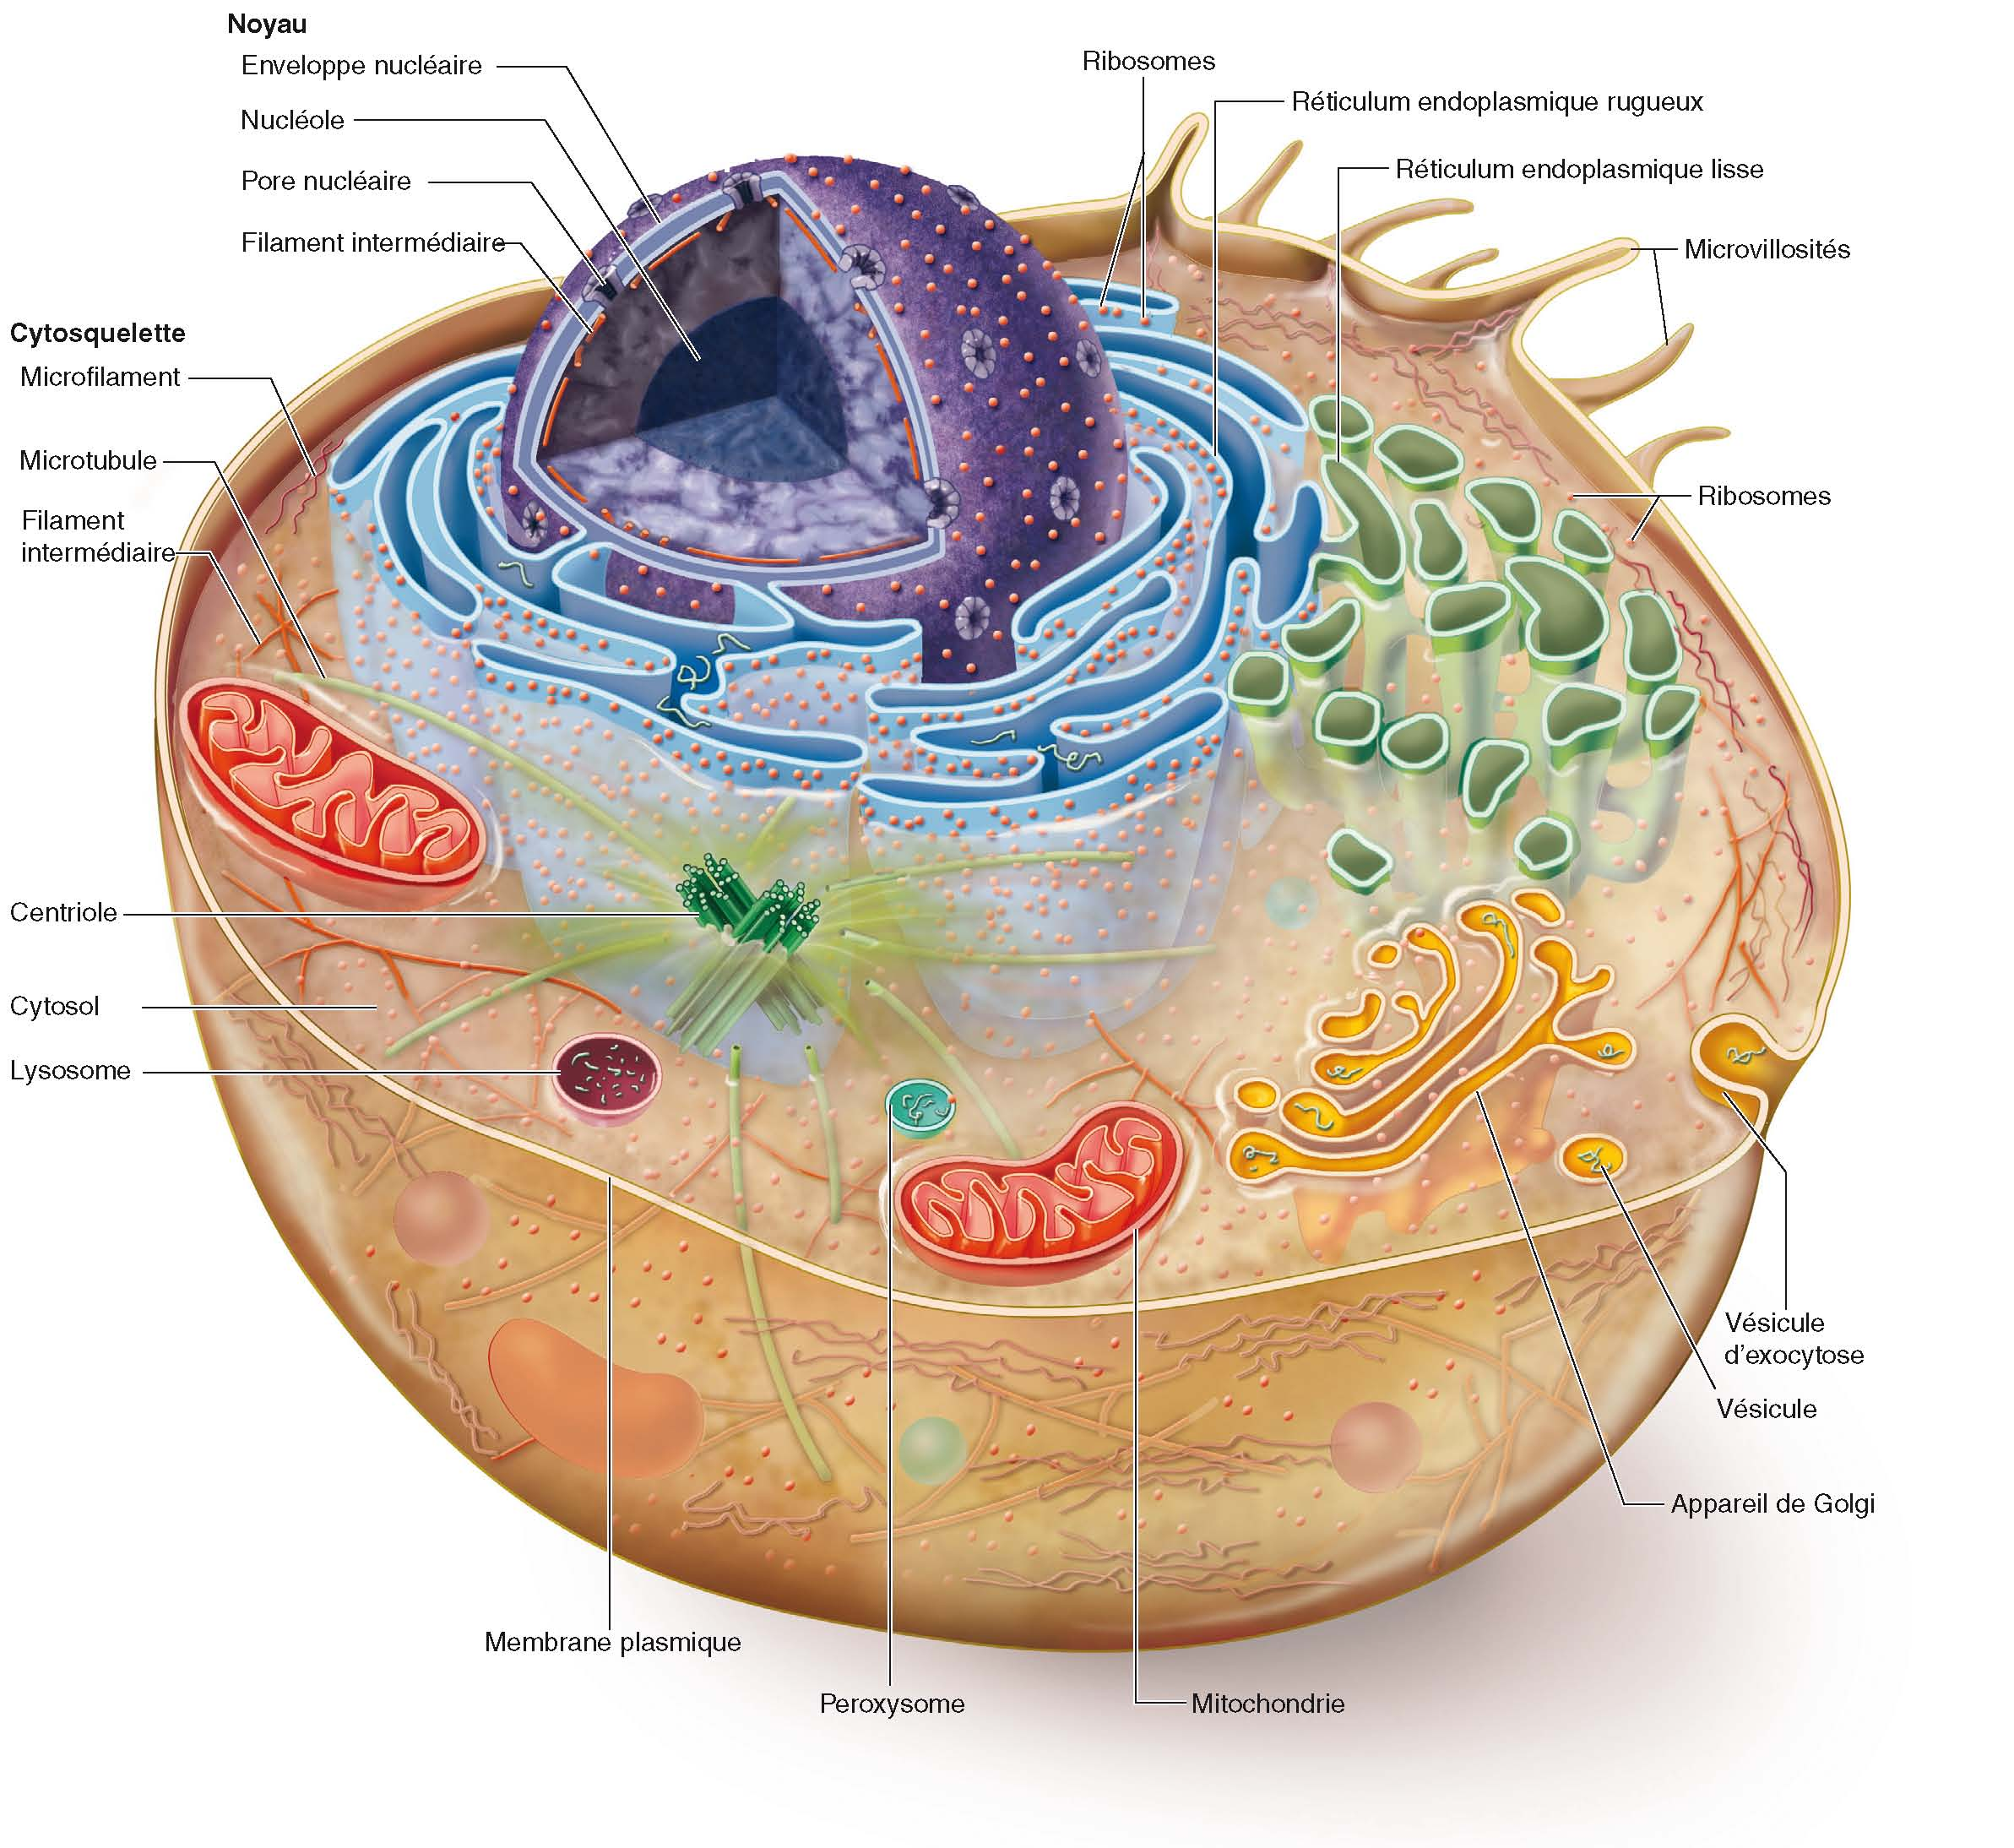
\includegraphics[width=1.0\linewidth]{./figures/ch1/cellule}}
    \caption[Cellule eucaryote]{\it Cellule eucaryote en coupe horizontale  \cite{johnson2011biologie}.}
    \label{Fig:cellule}
  \hspace{0.2cm}
\end{figure}

\section{Acteurs et processus de la biologie moléculaire}

Les biomolécules sont impliquées dans le fonctionnement des organismes vivants et plus particulièrement de leur sous-unité la plus importante : la cellule. On retrouve parmi ces biomolécules, les \textbf{molécules d'eau}, qui constituent souvent la part majoritaire dans la composition des organismes, les \textbf{lipides}, qui sont les composants de base des membranes cellulaires permettant de créer des cloisons et compartiments, les \textbf{acides nucléiques} qui sont les constituants de l'ARN et de l'ADN, 
support de l'information génétique, les \textbf{acides aminés} qui forment les protéines, principaux acteurs du fonctionnement cellulaire, les \textbf{sucres} qui jouent un rôle fondamental dans de nombreux processus, puis diverses autres molécules, par exemple des co-facteurs comme l'hème.

Nos travaux de recherche portent sur les biomolécules de plus grande taille, appelées également macromolécules, comme l'ADN et les protéines. L'information génétique stockée dans l'ADN est transmise et conservée de génération en génération grâce à la reproduction. Les protéines, sont à la fois les ouvriers, les briques et les messagers impliqués dans le fonctionnement cellulaire. Nous porterons une attention particulière aux édifices macromoléculaires composés de plusieurs protéines appelés complexes protéiques, même si les résultats de nos travaux de recherches s'appliquent à une large gamme de biomolécules, des plus simples aux plus complexes.

\subsection{Les biomolécules au coeur de la machinerie cellulaire}

L'information génétique (génotype), est un plan dont l'exécution conditionne l'apparence d'un être vivant, son fonctionnement, et son comportement dans son environnement (phénotype). Cette information génétique est stockée de manière pérenne et reproductible sur un support de nature moléculaire : l'\textbf{ADN} pour Acide Desoxyribo-Nucléique ou l'\textbf{ARN} pour Acide Ribo-Nucléique. L'ADN est porté par les chromosomes, situés dans le noyau de la cellule (voir Figure \ref{Fig:cellule}).
L'exécution de ce plan s'effectue à l'échelle moléculaire et commence par la lecture de l'information génétique dans le noyau et se termine par la production de toutes les protéines dans le cytoplasme (voir Figure \ref{Fig:cellule}). Ce processus de transformation de l'information génétique en des composants fonctionnels est commun à tous les êtres vivants.

Le fonctionnement d'une cellule vivante implique aussi d'autres acteurs. Parmi ces molécules, les \textbf{polysaccharides} et les \textbf{lipides} ne sont pas générées par le code génétique mais jouent un rôle prépondérant dans la structuration, notamment de la membrane cellulaire (voir Figure \ref{Fig:cellule}), d'autres stockent l'énergie nécessaire à la cellule et enfin certaines fonctionnent comme messagers inter- et intra-cellulaires.

%\begin{figure}
%  \centering
%  {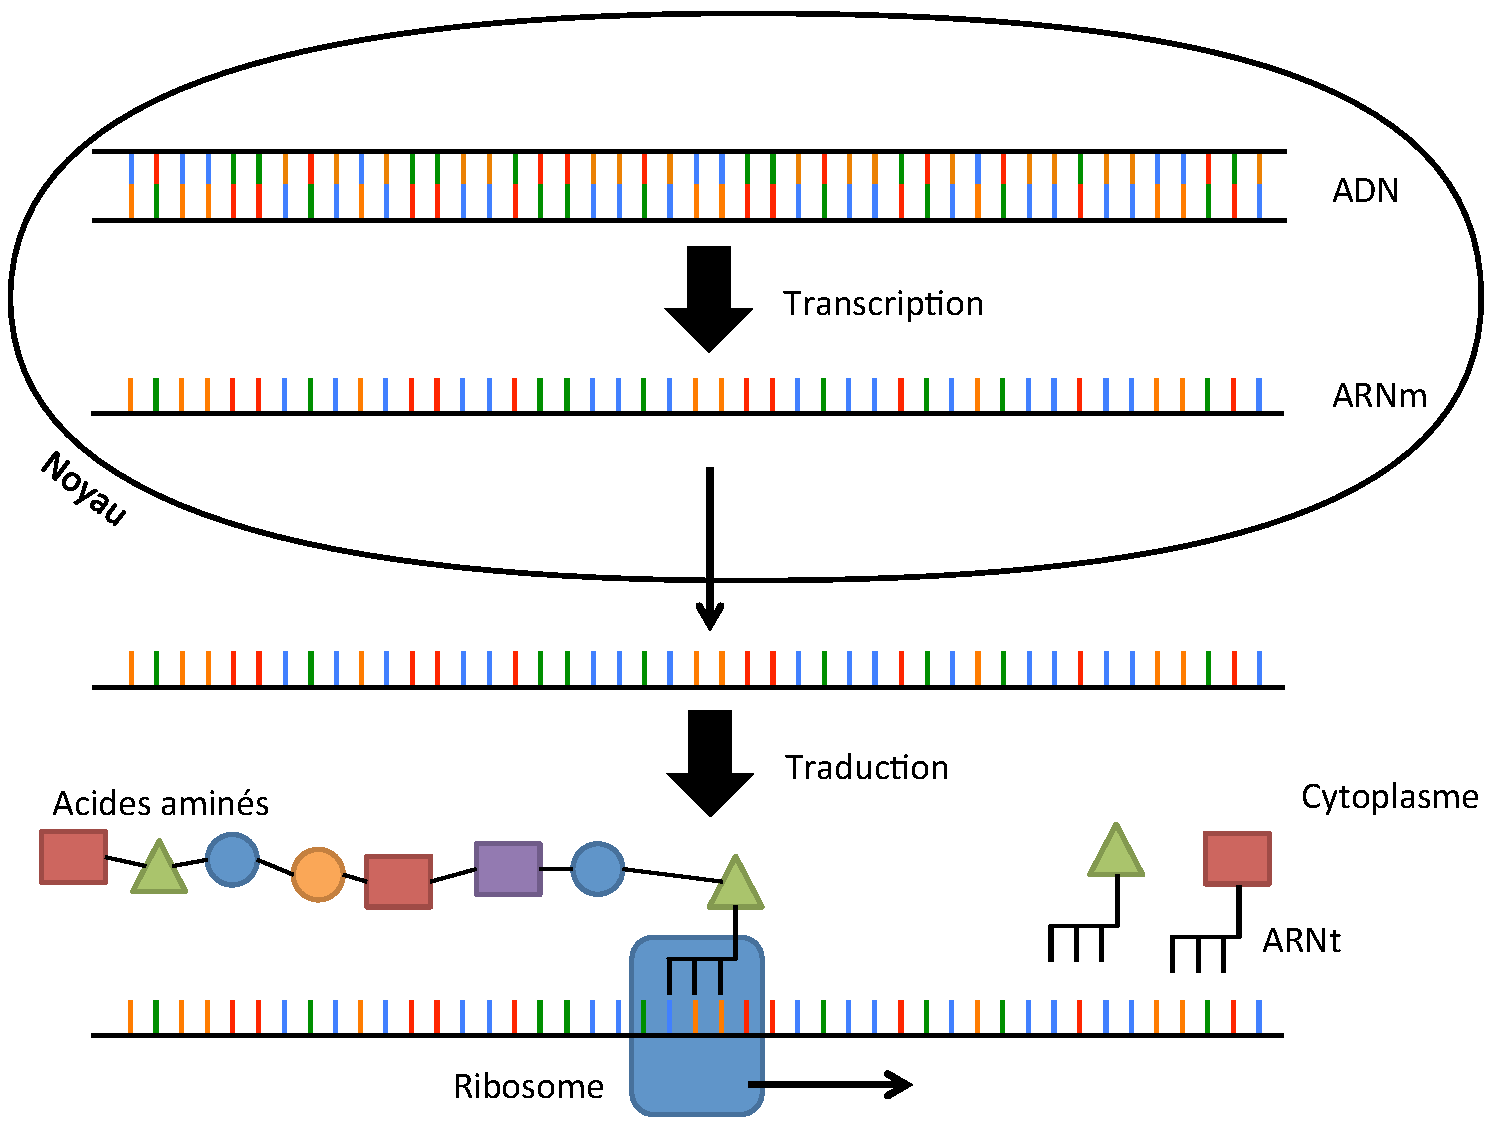
\includegraphics[width=.75\linewidth]{./figures/ch1/transc_trad.pdf}}
%    \caption{\it Schéma des processus de transcription et de traduction. L'ADN est transcrit en ARN dit <<messager>> afin de traverser la membrane du noyau et pénétrer dans le cytosplame où elle sera traduite par le ribosome afin de créer une séquence d'acides aminés, la protéine.}
%  \label{Fig:transc_trad}
%  \hspace{0.2cm}
%\end{figure}


\begin{figure}
  \begin{subfigure}{.6\textwidth}
  \centering
  {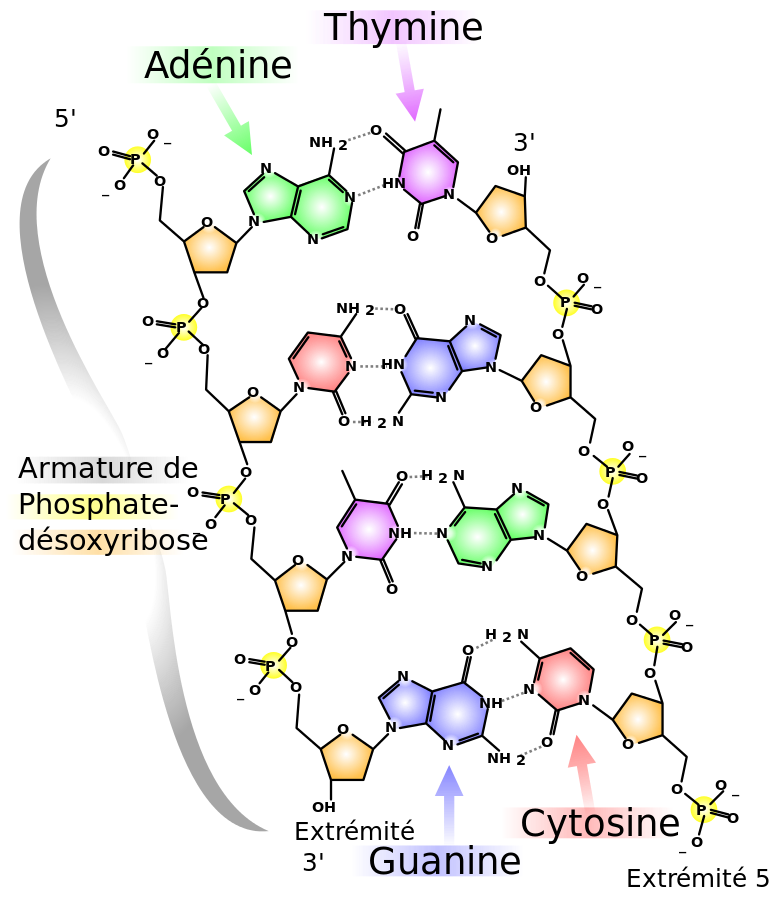
\includegraphics[height=6cm]{./figures/ch1/dna_structure}}
    \caption{}
    \label{Fig:dna_structure}
  % \hspace{0.2cm}
  \end{subfigure}
  \begin{subfigure}{.4\textwidth}
  \centering
  {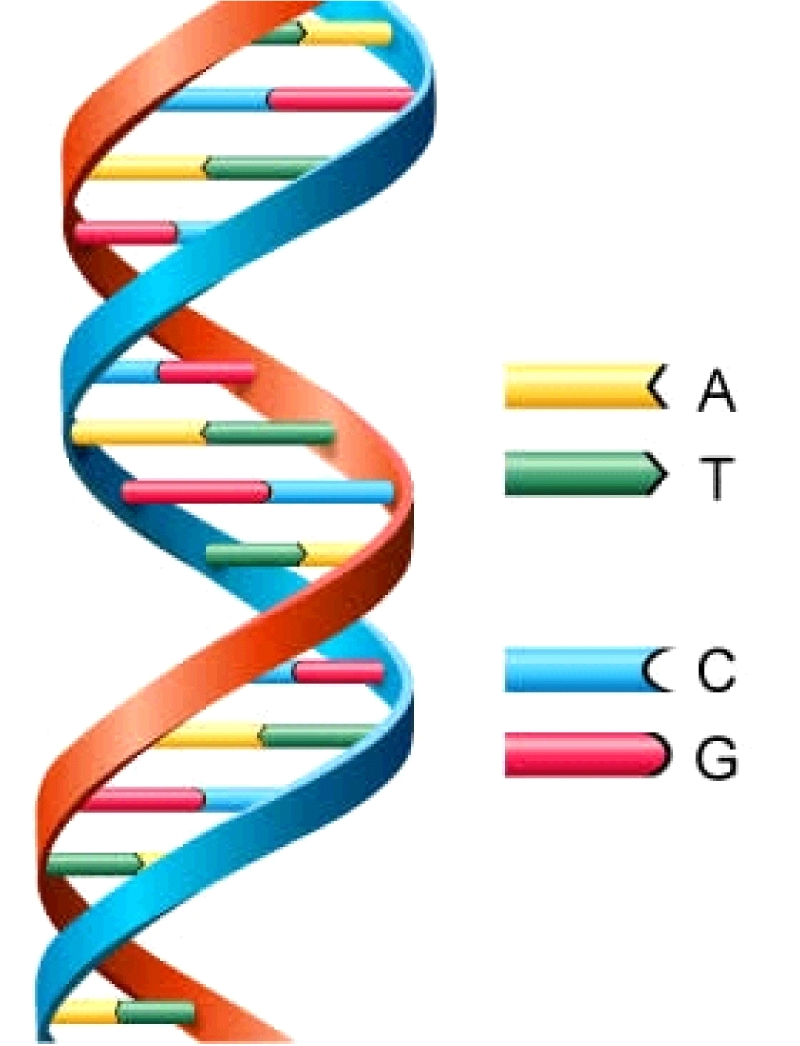
\includegraphics[height=6cm]{./figures/ch1/dna_structure_3d}}
    \caption{}
    \label{Fig:dna_structure_3d}
  % \hspace{0.2cm}
  \end{subfigure}
  \caption[(a) Structure ADN 2d / (b) Structure ADN 3d]{\it (a) Structure chimique de l'ADN mettant en jeu la liaison de nucléotides Adénine (en vert) avec Thymine (en rose) et Cytosine (en rouge) avec Guanine (en violet). Le squelette de l'ADN est composé par la liaison de Phosphates (en jaune) avec un groupement désoxyribose (en orange). Source : \cite{en:user:madprime_dna_chemical_structure_fr_2007}
  (b) Représentation simplifiée de l'ADN en 3d, chaque type de nucléotides étant représenté par une couleur différente.}
  % \hspace{0.2cm}
\end{figure}

\subsubsection{L'ADN}

L'Acide Désoxyribo-Nucléique (ADN) est une biomolécule pouvant être considérée comme le plan de construction de tous les êtres vivants. Le support moléculaire contenant l'information génétique est une longue séquence de nucléotides, de quatre types : l'Adénine, la Thymine, la Guanine et la Cytosine. Ces nucléotides partagent une structure moléculaire commune constituée d'un sucre, le désoxyribose, et d'un groupe phosphate (voir Figure \ref{Fig:dna_structure}). À cette partie commune se lie une base azotée spécifique à chacun des 4 types de nucléotides. Les nucléotides s'organisent en séquence de deux brins en complémentarité en établissant des liaisons hydrogène spécifiques. L'Adénine et la Guanine se liant respectivement à la Thymine et la Cytosine.

\begin{figure}[htb]
 \centering
 {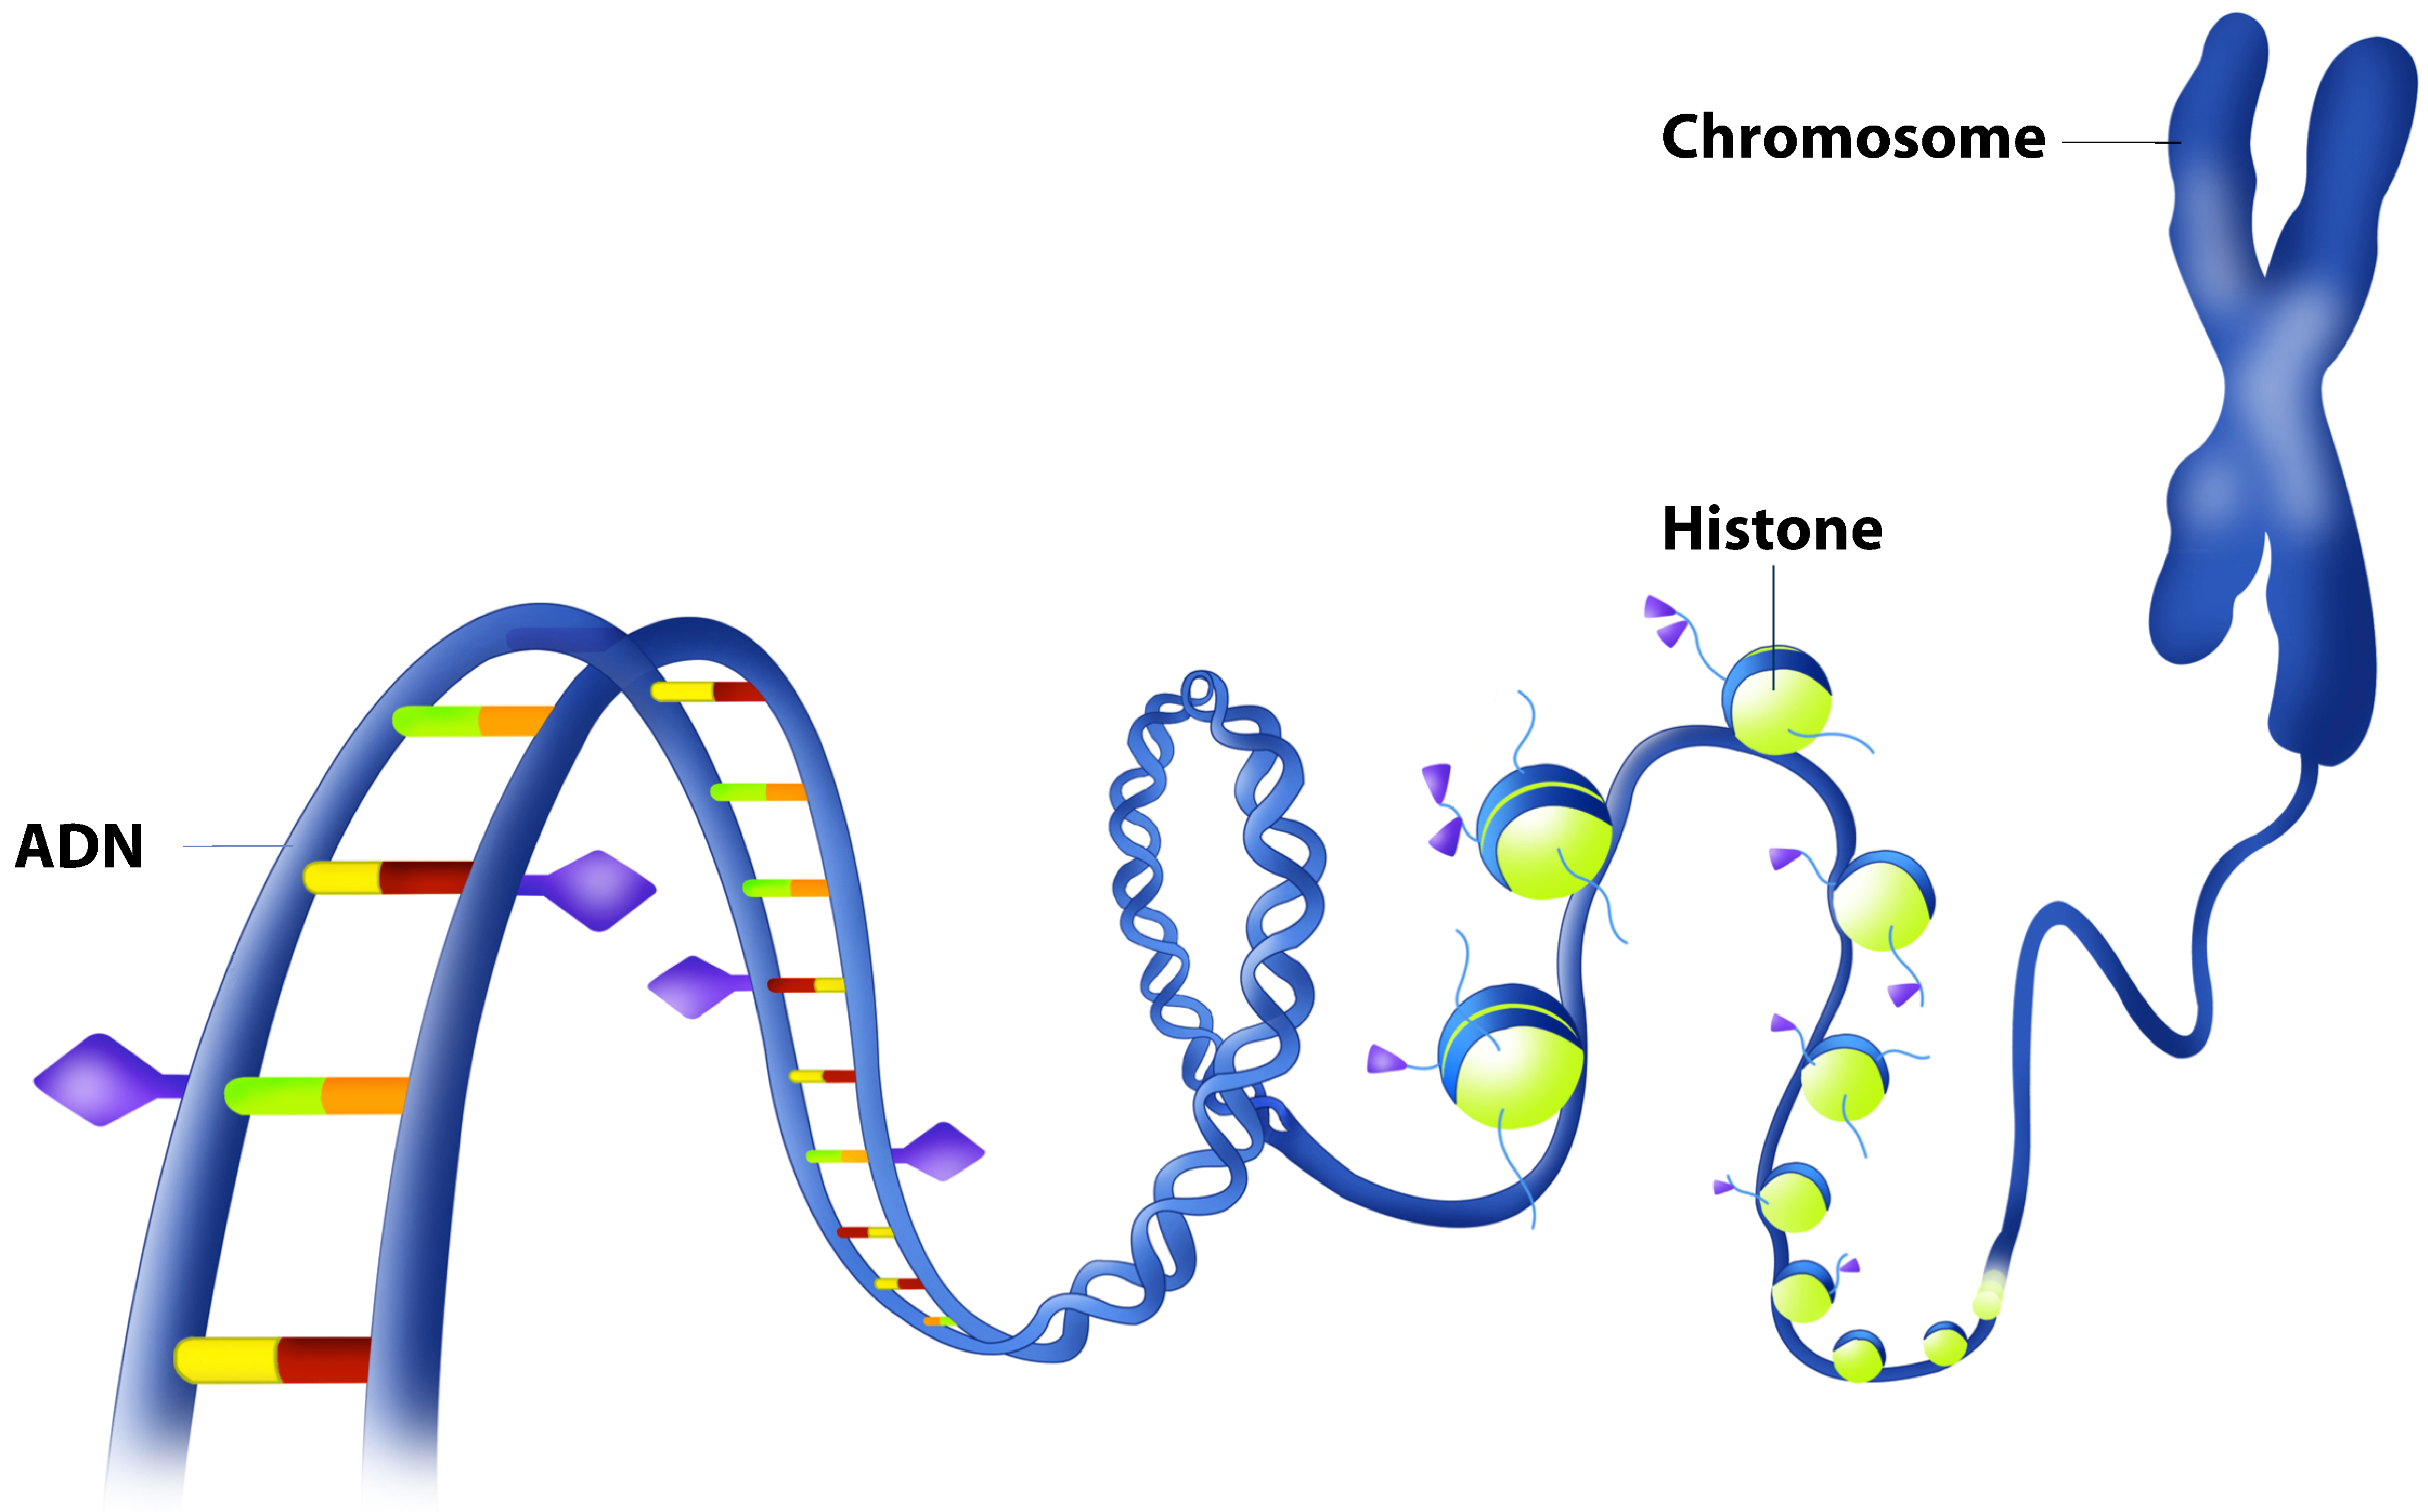
\includegraphics[width=0.6\linewidth]{./figures/ch1/chromosome_adn_horizontal.pdf}}
   \caption[Echelles de structuration du chromosome à l'ADN]{Les différentes échelles de structuration d'un chromosome, forme condensée de l'ADN. Ce chromosome est lui-même composé d'ADN enroulé autour de protéines structurantes, les histones. Source : NIGMS\footnote{\url{http://images.nigms.nih.gov/index.cfm?event=viewDetail&imageID=2563}}}
   \label{Fig:chromosome_adn_2}
  \hspace{0.2cm}
\end{figure}

Les deux brins de l'ADN adoptent une structure hélicoïdale. Leur complémentarité permet tout d'abord d'assurer une certaine résistance de la structure à la dégradation et, en cas d'endommagement d'un des deux brins, la redondance de la complémentarité permet la réparation du brin intact.
L'ADN est lui-même structuré de façon plus complexe, d'abord compacté par les histones (voir Figure \ref{Fig:cellule}), protéines structurantes possédant une forte affinité avec l'ADN qui s'enroule autour, puis finalement organisés en superstructures, les chromosomes. 
Chez les eucaryotes, organismes pluricellulaires possédant un noyau dans la cellule, l'ADN est stocké dans le noyau \cite{johnson2011biologie}. 


\subsubsection{L'ARN}

L'Acide RiboNucléique (ARN) est une biomolécule structurellement proche de l'ADN comportant néanmoins quelques différences. La première se retrouve au niveau de la séquence d'acides nucléiques qui, contrairement à l'ADN, très majoritairement composé d'un double brin sous forme d'hélice, s'organise en simple brin. Une seconde différence concerne les sucres constituant chacun des nucléotides puisque le désoxyribose de l'ADN est remplacé par un ribose pour l'ARN. La différence entre les deux groupements est illustrée dans la Figure \ref{Fig:desoxyribose_vs_ribose}. De plus, la Thymine présente dans l'ADN n'existe pas dans l'ARN et est remplacée par l'Uracile, complémentaire, comme la Thymine, à l'Adénine.

\begin{figure}[htb]
  \centering
  {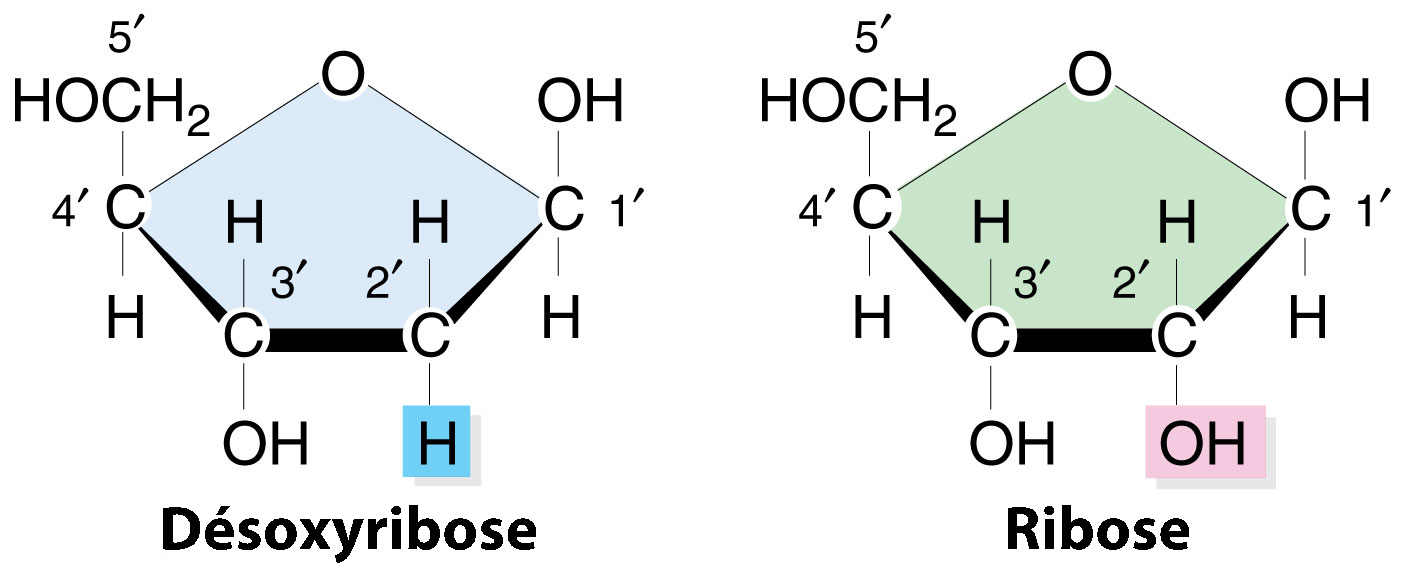
\includegraphics[width=0.8\linewidth]{./figures/ch1/desoxyribose_vs_ribose}}
    \caption[Comparaison composition chimique ADN/ARN]{\it Composition chimique d'un désoxyribose, présent dans l'ADN, mis en parallèle avec un ribose, présent dans l'ARN. La seule différence provient du groupement hydrogène présent sur le carbone 2 du désoxyribose qui est remplacé par une groupement hydroxyle dans le ribose. Source: \cite{russel2010igenetics}
    % \commentaire{MB: il serait bien d'indiquer la notation courte et symbolique de ces deux sucres (voir le site glycopedia de Serge); Thibault Tubiana peut certainement aider la-dessus; c'etait une partie de son sujet de stage}
    }
    \label{Fig:desoxyribose_vs_ribose}
  \hspace{0.2cm}
\end{figure}

%En dehors de l'ARN messager, responsable de la transmission de l'information génétique portée de l'ADN depuis le noyau jusqu'au cytoplasme après la transcription, il existe d'autres type  d'ARNs présentés succinctement ci-dessous de manière non exhaustive, dont le rôle sera explicité dans la description des étapes de transcription et de traduction dans la section \ref{trans_trad}.

%L'\textbf{ARNt}, ou ARN de transfert, sont des ARN de petite taille qui permettent le transport des acides aminés vers le ribosome lors de la traduction.
%Les \textbf{ARN catalytiques} regroupent les ARN possédant un rôle catalytique dans la cellule. Ils interviennent par exemple pour des étapes d'épissage de l'ARNm pendant son étape de maturation, certains ARN de virus peuvent se cliver eux-mêmes et sont donc potentiellement indépendants alors que d'autres peuvent catalyser certaines réactions chimiques et de fixer certaines molécules.
%Les \textbf{ARN guides} sont des ARN s'associant à des enzymes protéiques afin de diriger leurs actions vers des ARN ou des ADN de séquences complémentaires.
%Les \textbf{ARN régulateurs} ont pour cible les ARNm sur lesquels ils se lient par complémentarité. Cette liaison peut empêcher la traduction de l'ARNm cible par les ribosomes ou bien agir sur la stabilité de l'ARNm régulant ainsi son expression (positivement ou négativement).

\subsubsection{Les protéines}


Les protéines sont les biomolécules considérées comme les acteurs moléculaires fonctionnels de la cellule. Les protéines sont à la fois les briques, les ouvriers et les messagers participant au fonctionnement cellulaire. Les règles qui régissent la production de protéines à partir de la lecture de l'information génétique sont décrites dans le code génétique universel, commun à tous les organismes vivants. Certaines assurent un rôle \textbf{structurel}, en étant notamment impliquées dans la construction et la structure du squelette de la cellule, comme l'actine et le collagène qui assurent le maintien physique et structurel de la cellule ainsi que la résistance de la matrice extracellulaire. Certaines sont impliquées dans la \textbf{mobilité} des cellules et des organismes, comme les myosines qui permettent la contraction musculaire, transformant l'énergie chimique en énergie mécanique. Certaines jouent un rôle dans le \textbf{conditionnement de l'ADN}, l'ADN étant enroulé autour de protéines appelées les histones (voir Figure \ref{Fig:chromosome_adn_2}), d'autres sont impliquées dans la \textbf{régulation de l'expression génétique}, comme les facteurs de transcription accompagnant l'ARN polymérase lors de la transcription. Certaines font office de \textbf{transporteurs} du matériel cellulaire d'un point à un autre, comme la kinésine évoluant sur des structures de microtubules (cf. Figure \ref{Fig:kinesincargoart}).

\begin{figure}[h]
  \centering
  {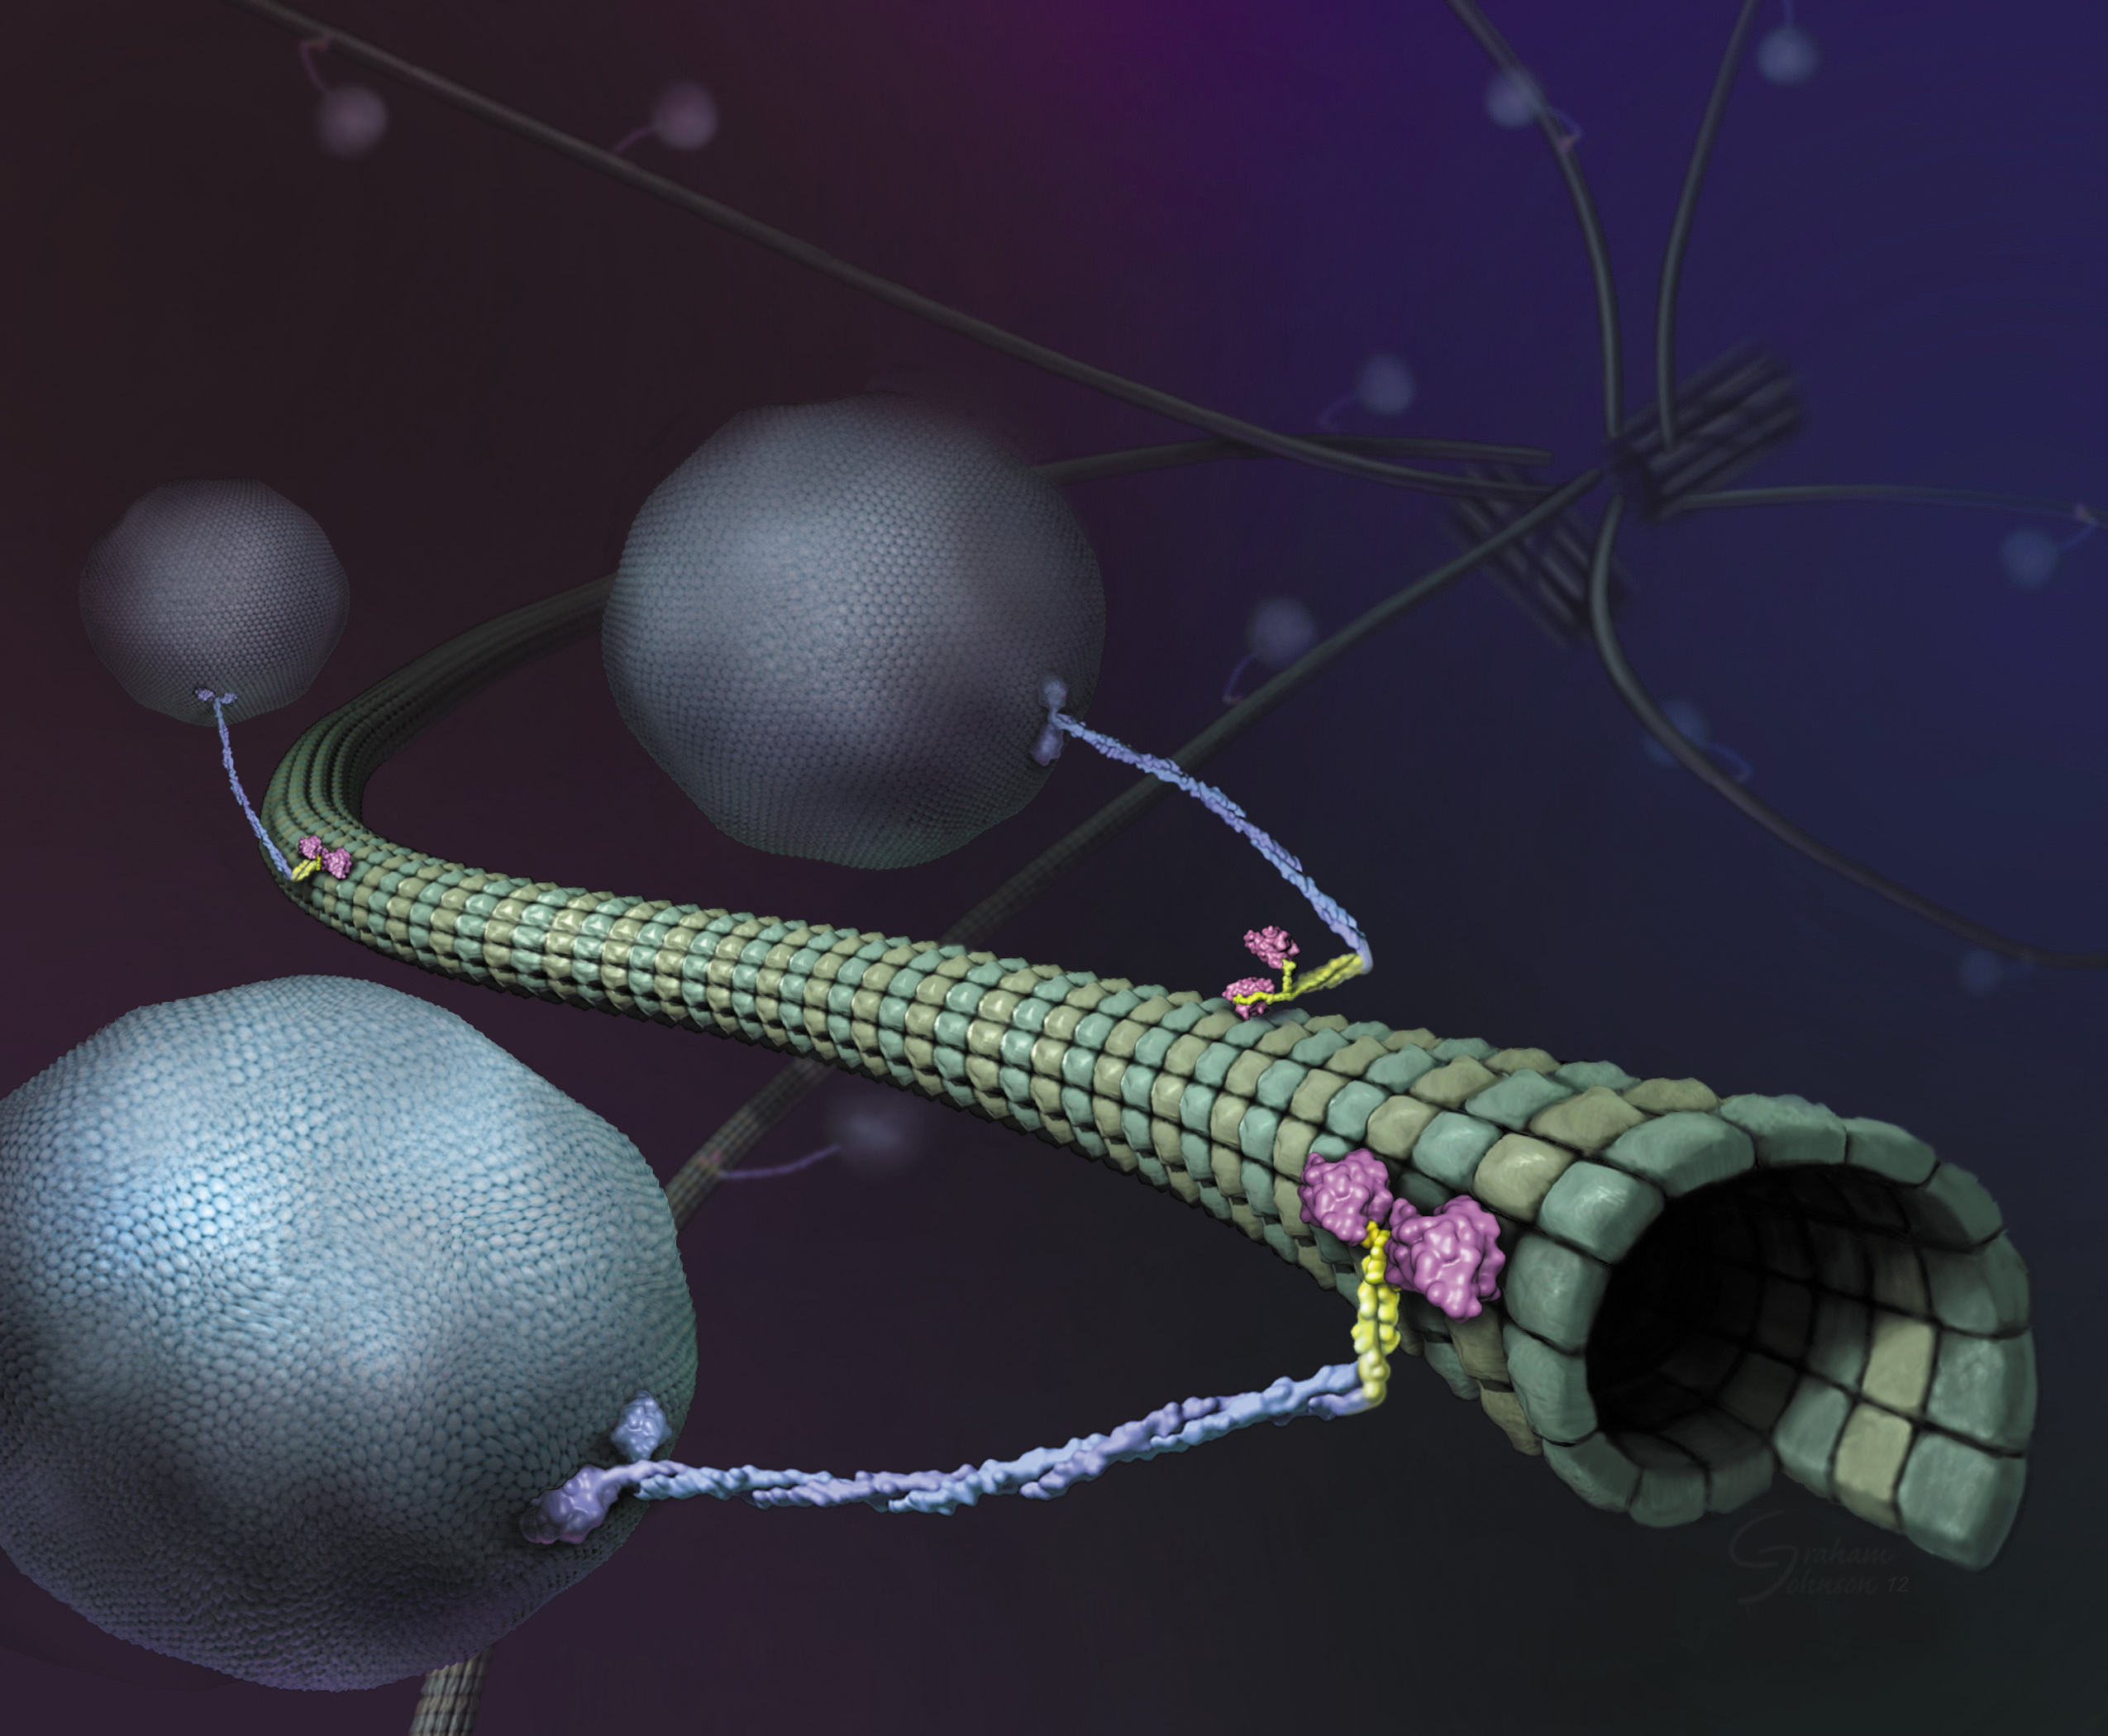
\includegraphics[width=0.75\linewidth]{./figures/ch1/kinesincargoart}}
    \caption[Vue d'artiste du transport de vésicules le long de microtubules]{\it Vue d’artiste du transport de vésicules contenant du matériel cellulaire (boules blanches et bleues) le long de microtubules (tube de couleur verte) par une protéine appelée kinésine. La kinésine est composée de plusieurs domaines : en rose les deux domaines constituant les <<jambes>> de la protéine, en bleu un filament dont le domaine terminal se lie aux vésicules proches. A la frontière entre les domaines jaunes et roses, la transformation de l'énergie chimique en énergie mécanique permet à la protéine de <<marcher>> sur les microtubules. Source: Graham Johnson (graham@grahamj.com) / modifié de "Journal of Cell Biology, November 27, 2000"}
    \label{Fig:kinesincargoart}

\end{figure}

% \begin{figure}
%   \centering
%   {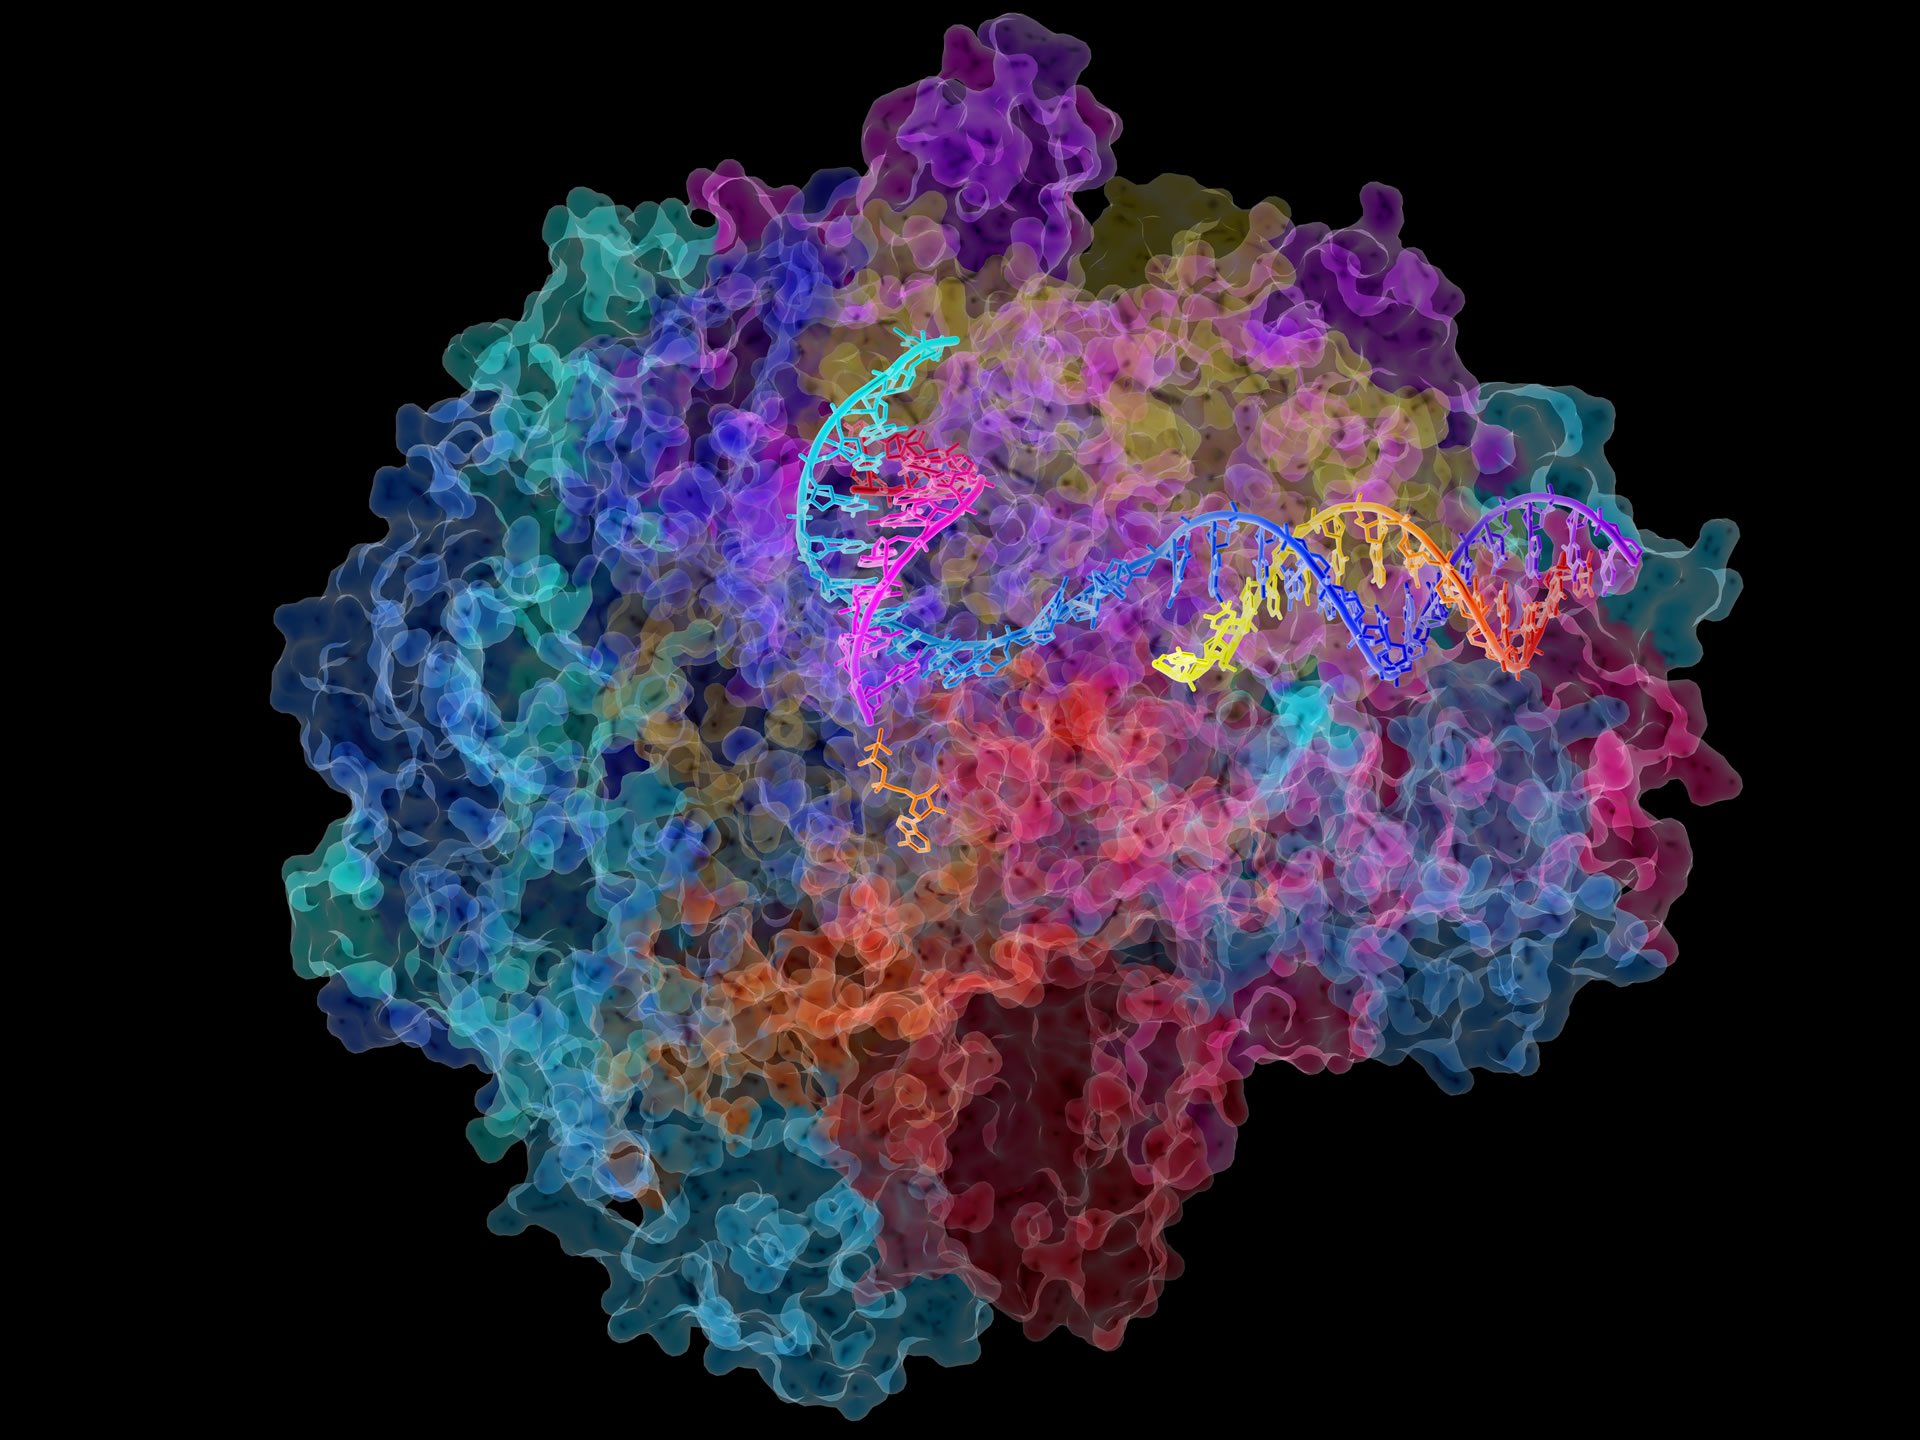
\includegraphics[width=0.5\linewidth]{./figures/ch1/RNA_pol_II}}
%     \caption{\it ARN polymérase liée à un fragment d'ADN. La protéine est représentée sous forme de surface transparente de couleur alors que l'ADN est représentée sous forme de bâtons opaques.}
%     \label{Fig:RNA_pol_II}
%   \hspace{0.2cm}
% \end{figure}

Une protéine est constituée d'une succession d'acides aminés liés entre-eux dont il existe 22 sortes différentes. Les acides aminés sont composés d'atomes de carbone, d'hydrogène, d'oxygène et d'azote, certains intégrant aussi un atome de soufre ou de sélénium. Ces acides aminés possèdent une partie commune, le squelette, et une partie spécifique appelée la \textit{chaîne latérale}, qui caractérise le type d'acide aminé. C'est au niveau de la partie commune que les acides aminés sont liés par une \textit{liaison peptidique}, la séquence des parties communes constituant la \textit{chaîne principale} (ou squelette) de la protéine (cf. Figure \ref{Fig:amino_acid_structure} et \ref{Fig:peptide_bond}). La chaîne latérale spécifique à chaque type d'acide aminé donne lieu à des propriétés physico-chimiques différentes. Chaque acide aminé peut être représenté par la formule générique H$_{2}$N-HC$R$-COOH, dans laquelle $R$ désigne la chaîne latérale (cf. Figure \ref{Fig:amino_acid_structure}).

\begin{figure}[htb]
  \begin{subfigure}{.4\textwidth}
  \centering
  {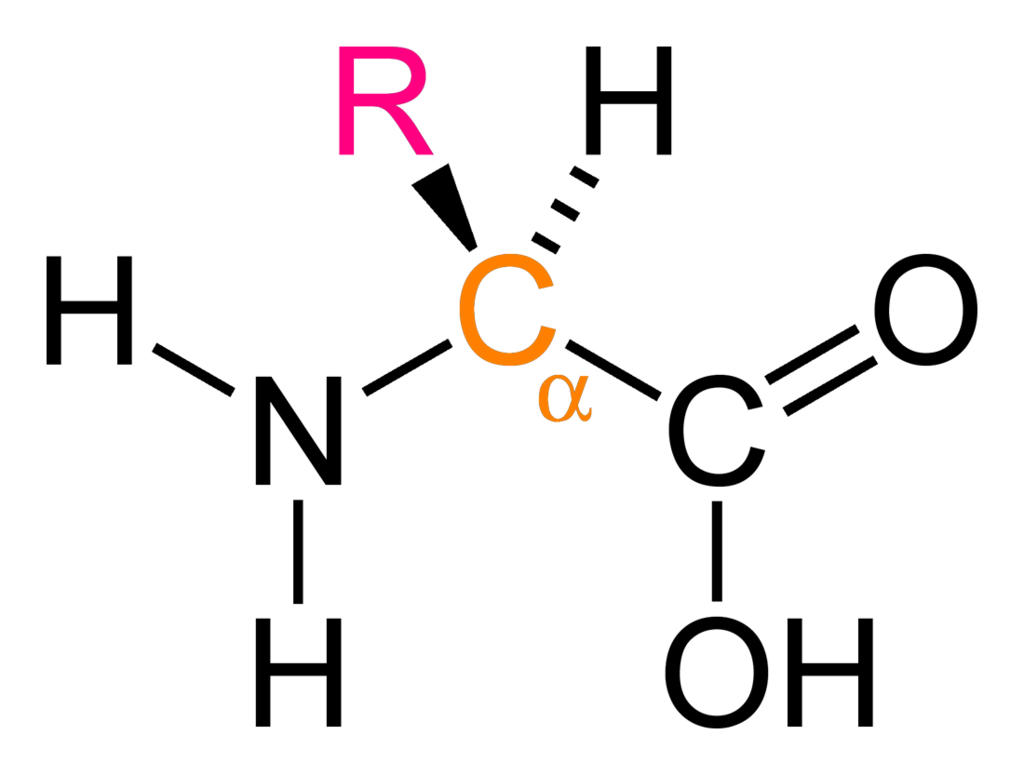
\includegraphics[height=4cm]{./figures/ch1/amino_acid_structure}}
    \caption{}
    \label{Fig:amino_acid_structure}
  % \hspace{0.2cm}
  \end{subfigure}
  \begin{subfigure}{.6\textwidth}
  \centering
  {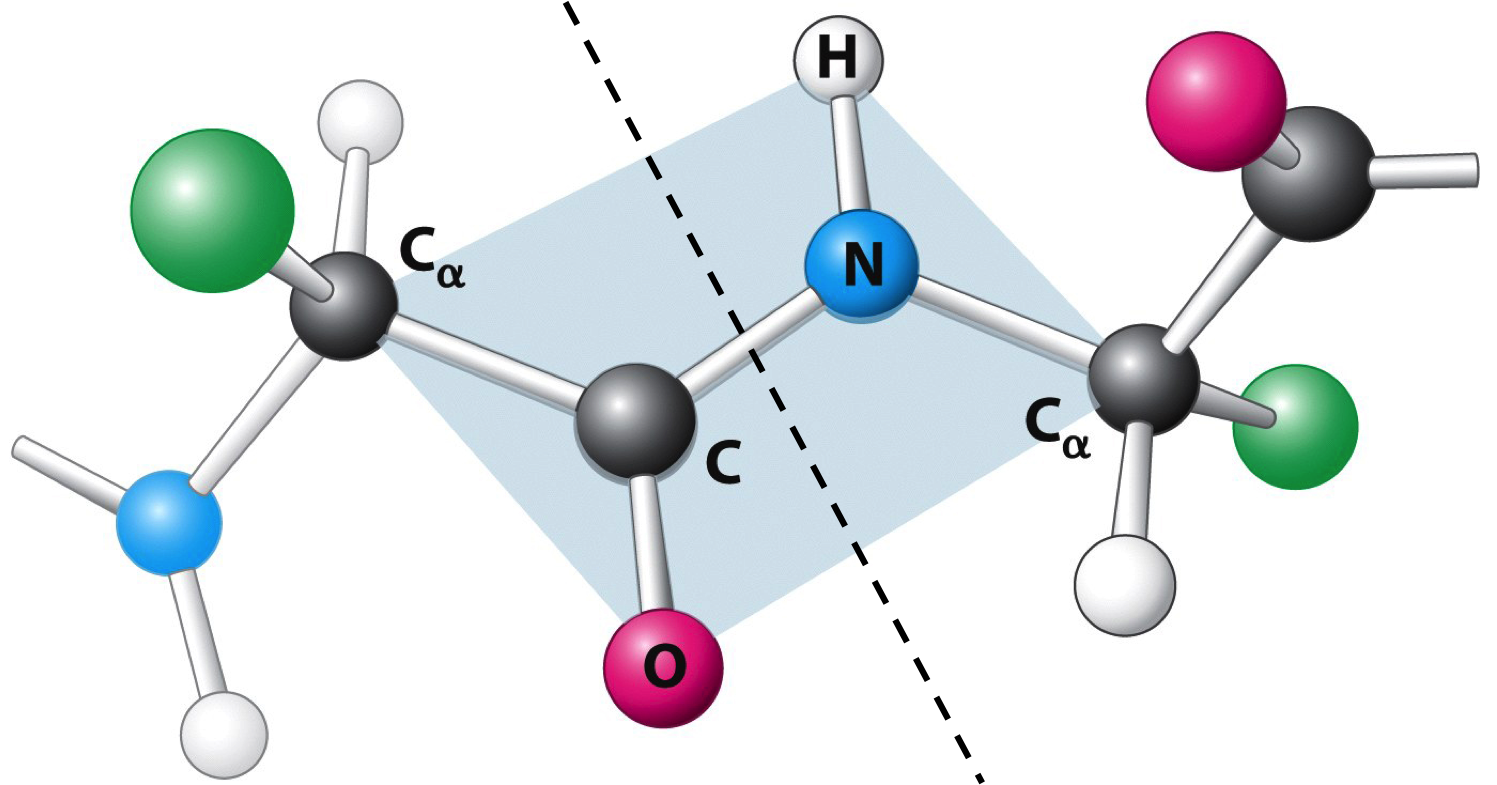
\includegraphics[height=4cm]{./figures/ch1/peptidic_bond.png}}
    \caption{}
    \label{Fig:peptide_bond}
  % \hspace{0.2cm}
  \end{subfigure}
  \caption[(a) Structure chimique d'un acide aminé. (b) Illustration d'une liaison peptidique entre deux acides aminés.]{\it (a) Structure chimique d'un acide aminé. En jaune est représenté le Carbone alpha où est lié la chaîne latérale dont la composition atomique est différente suivant le type d'acide aminé.
  (b) Illustration d'une liaison peptidique entre deux acides aminés (à gauche et à droite de la ligne pointillée). Cette liaison est une liaison covalente entre l'azote (N) du groupe amide de l'acide aminé de droite et le carbone (C) du groupe carboxyle de l'acide aminé de gauche. En vert sont représentés les chaînes latérales simplifiées. Source: \cite{berg_biochemistry_2012}}
\end{figure}
% \begin{figure}
%   \centering
%   {\includegraphics[width=0.75\linewidth]{./figures/ch1/amino_acids_type}}
%     \caption{\it Représentation des différents acides aminés classés selon leurs propriétés physico-chimiques. Cette classification n'est pas universelle et d'autres regroupements basés sur d'autres propriétés peuvent être proposés.}
%     \label{Fig:amino_acids_type}
%   \hspace{0.2cm}
% \end{figure}


Il est possible de classer les acides aminés selon plusieurs critères, depuis leur taille jusque leur propriété hydrophile (affinité avec l'eau) ou leur polarité. Il existe cependant un classement commun qui les regroupe en six groupes fonctionnels : Les acides aminés \textbf{aliphatiques} (Glycine, Alanine, Valine, Leucine et Isoleucine), les acides aminés avec groupement \textbf{hydroxyle, sulfurique ou sélénique} (Sérine, Thréonine, Méthionine, Cystéine et Sélénocystéine), les acides aminés \textbf{cycliques} (Proline), les acides aminés \textbf{aromatiques} (Phénylalanine, Tyrosine et Tryptophane), les acides aminés \textbf{basiques} (Histidine, Lysine et Arginine) et enfin les acides aminés \textbf{acides} et leurs \textbf{amides} (Aspartate, Glutamate, Asparagine et Glutamine) (voir Figure \ref{Fig:diagramme_venn}).

\begin{figure}[!htb]
  \centering
  {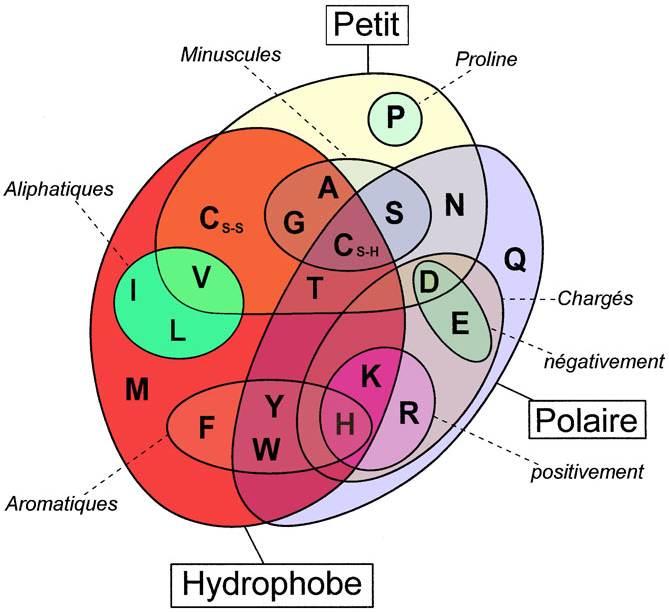
\includegraphics[width=0.55\linewidth]{./figures/ch1/diagramme_venn}}
    \caption[Diagramme de Venn illustrant les différentes classifications servant à définir les acides-aminés.]{\it Diagramme de Venn illustrant les différentes classifications servant à définir les acides-aminés. Ces propriétés peuvent être structurelles (minuscules, petit) ou physico-chimiques (polaire, hydrophobe, etc.). 
    Source : \cite{wikipedia_francais_2006}
    }
    \label{Fig:diagramme_venn}
  % \hspace{0.2cm}
\end{figure}

La séquence des acides aminés, pouvant être représentée par une suite de lettres choisies parmi un alphabet de 22 lettres correspondantes chacune à un type d'acide aminé, est appelée la \textbf{structure primaire} d'une protéine.

La protéine va adopter, contrainte par les interactions physiques et chimiques entre les différents atomes de la chaîne principale et latérale, des structurations locales particulières. Ces motifs structuraux formés sont au nombre de 3 : \textit{hélices}, \textit{feuillets} et \textit{coudes} et leur enchaînement est appelé la \textbf{structure secondaire} de la protéine (voir Figure \ref{Fig:secondary_structure}).

Enfin, les protéines possèdent également des motifs plus importants, souvent le résultat de l'agencement dans l'espace des motifs de structures secondaires cités précédemment. C'est la \textbf{structure tertiaire} ou structure tridimensionnelle de la protéine (cf. Figure \ref{Fig:tertiary_structure}). 
Cette structuration est due aux interactions proches et longue distance formées par les chaînes latérales des acides aminés. Parmi ces interactions, on retrouve les attractions/répulsions électrostatiques des acides aminés chargés électriquement, l'effet hydrophobe est le phénomène d'enfouissement et de regroupement des régions dont le ratio d'acides aminés hydrophobes est important. Ces régions vont se retrouver à l'intérieur de la protéine alors qu'à l'inverse, les régions dites hydrophiles vont majoritairement se situer en surface de la protéine.
% Cette structure est maintenue par différents types d'interactions. Les interactions les plus fortes, appelées \textit{covalentes}, sont essentiellement le fait de ponts disulfures pouvant exister entre les atomes de souffre de deux Cystéines. Les interactions \textit{électrostatiques} regroupent les liaisons ioniques (entre cations et anions des chaînes latérales) et hydrogènes (entre oxygènes et hydrogènes de deux chaînes latérales). Les interactions de \textbf{Van der Waals} regroupent à la fois des forces de répulsion et d'attraction et sont des interactions faibles et à longue distance entre deux dipôles de charges électroniques fluctuantes et non liées. Enfin, les interactions \textbf{hydrophobes} sont un agencement des acides aminés par rapport à leur environnement. L'effet hydrophobe est le phénomène d'enfouissement et de regroupement des régions dont le ratio d'acides aminés hydrophobes est important. Ces régions vont se retrouver à l'intérieur de la protéine alors qu'à l'inverse, les régions dites hydrophiles vont majoritairement se situer en surface de la protéine.

% \commentaire{MB: pourquoi choisir les exemples suivants? On aurait pu en choisir d'autres, et ils ne correspondent pas aux ex. de la Fig. 1.8b si je ne me trompe pas.? -> J'ai enlevé les exemple pour ne pas qu'ils portent à confusion et un peu alléger le texte} 
% Parmi les agencements 3d récurrents, on peut citer le domaine \textit{immunoglobuline} qui est composé d'hélices et de feuillets et retrouvé en plusieurs exemplaires dans la structure des anticorps par exemple. Les \textit{tonneaux bêta} sont aussi courants et sont le résultat de l’enchaînement de feuillets bêta organisés de façon antiparallèle et formant un tonneau. Le motif \textit{hélice-coude-hélice} est également courant puisqu'il est un domaine de liaison à l'ADN et donc retrouvé dans les facteurs de transcription par exemple (voir Figure \ref{Fig:tertiary_structure}).

\begin{figure}[h]
  \begin{subfigure}{.4\textwidth}
  \centering
  {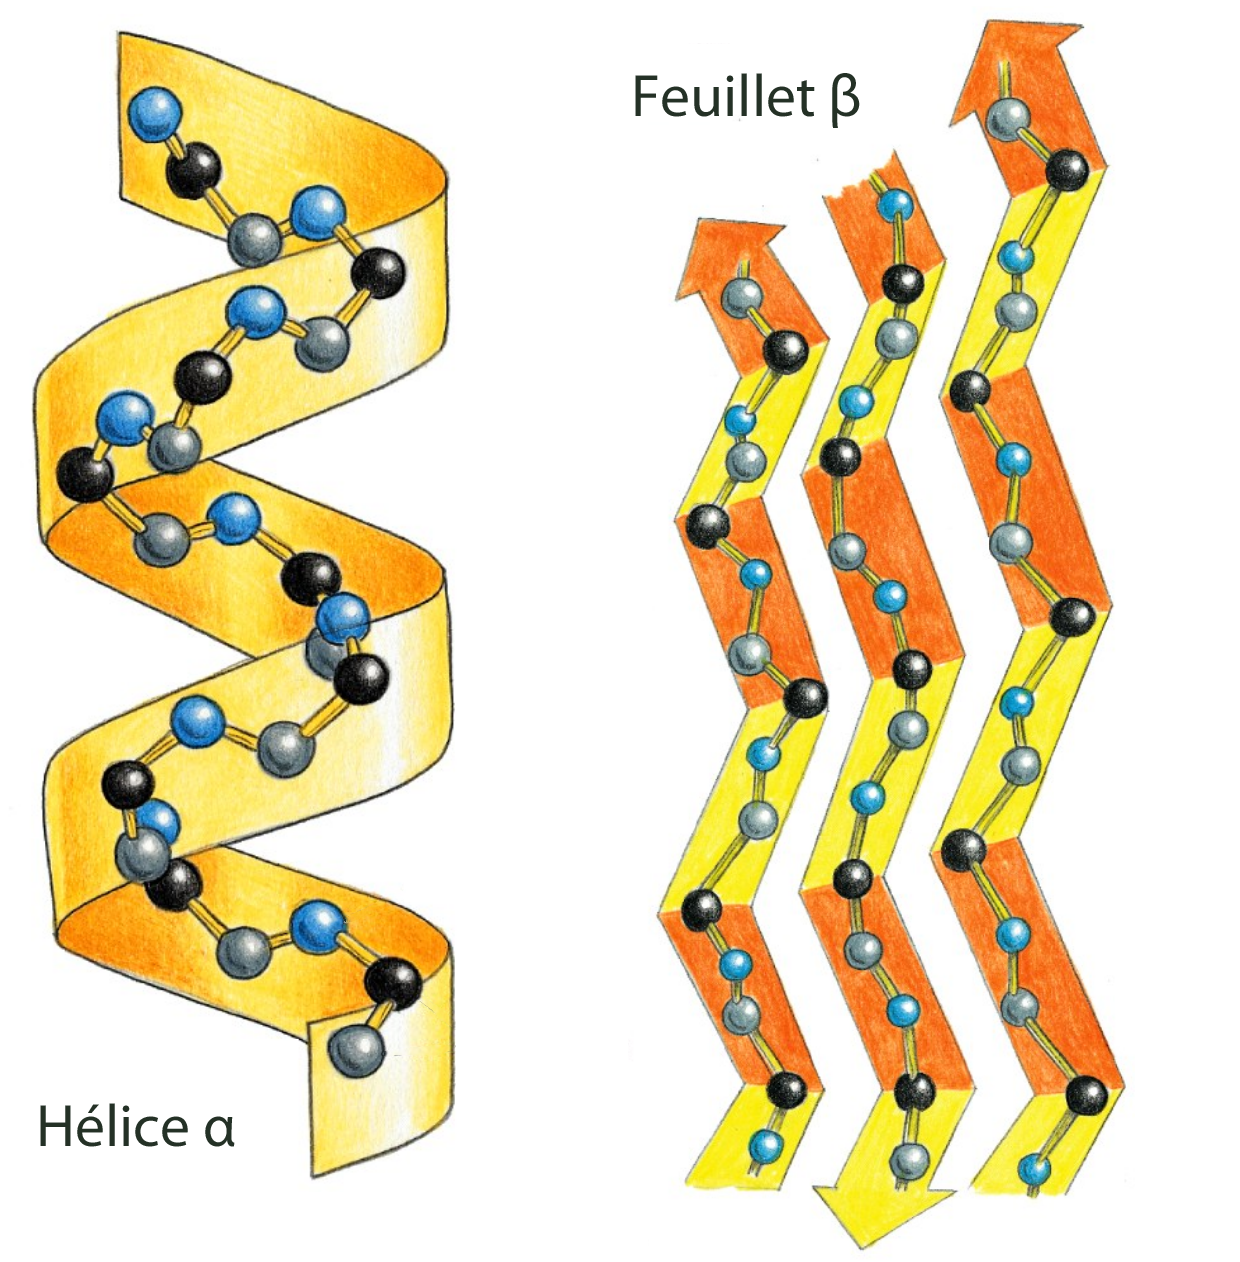
\includegraphics[width=0.9\linewidth]{./figures/ch1/secondary_structure.png}}
    \caption{}
    \label{Fig:secondary_structure}
  % \hspace{0.2cm}
  \end{subfigure}
  \begin{subfigure}{.6\textwidth}
  \centering
  {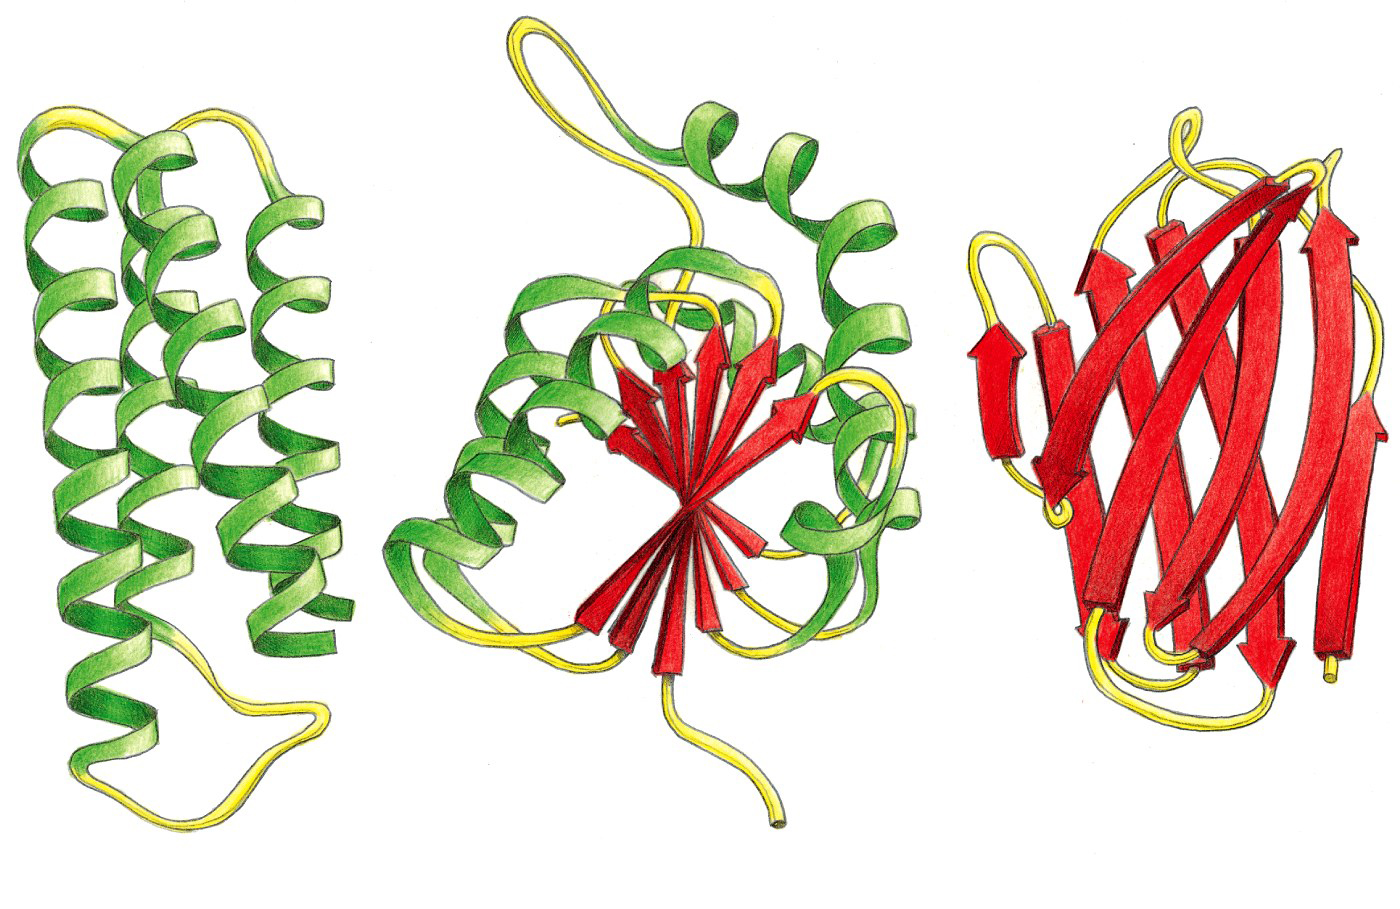
\includegraphics[width=\linewidth]{./figures/ch1/tertiary_structure.jpg}}
    \caption{}
    \label{Fig:tertiary_structure}
  % \hspace{0.2cm}
  \end{subfigure}
  \caption[(a) Représentation en rubans des motifs de structure secondaire. (b) Exemples de motifs communs de structures tertiaires.]{\it (a) Représentation en rubans des motifs de structure secondaire les plus communs, à gauche une hélice $\alpha$ et à droite un feuillet $\beta$, résultats de la configuration spatiale des atomes de la chaîne principale des protéines. Source : \cite{alberts2013essential}
  (b) Exemples de motifs communs de structures tertiaires. A gauche, représentation d'un paquet de 4 hélices $\alpha$ agencées autour du motif hélice-coude-hélice. Au centre, enchevêtrement d'hélices $\alpha$ et feuillets $\beta$. A droite, double couche de feuilles $\beta$. Dans ces illustrations sous forme de rubans de protéines, les hélices sont en vert, les feuillets en rouge et les coudes ou boucles en jaune. Source : \cite{alberts2013essential}
  }
  % \hspace{0.3cm}
\end{figure}

\subsubsection{Les polysaccharides}

Les polysaccharides, appelés aussi glucides complexes, sont des séquences répétées de sucres (ou oses). On peut distinguer deux groupes de polysaccharides qui se distinguent par leur fonction biologique. Les polysaccharides \textbf{de réserve} constituent une source d'énergie pour les êtres vivants. Ils se retrouvent principalement sous forme de \textit{glucose}.
Les polysaccharides \textbf{structuraux} participent eux à la formation des structures organiques comme la \textit{cellulose} dans les tissus de soutien chez les végétaux ou la \textit{chitine} chez les animaux (cf. Figure \ref{Fig:cell_membrane}).

A la différence des biomolécules citées précédemment, les polysaccharides, bien qu'indispensables aux cellules, ne sont pas synthétisées par ces dernières mais doivent être assimilés à travers la nourriture par exemple. De nombreuses informations à propos des polysaccharides, en particulier à propos de leur représentation et leurs structures sont rassemblées au sein du site Glycopedia\footnote{\url{http://www.glycopedia.eu/}}.

\subsubsection{Les lipides}

Les lipides constituent la matière grasse de l'organisme et englobent de nombreuses molécules différentes. Leur point commun réside dans la présence d'une partie hydrophobe même si celle-ci peut être liée à une partie hydrophile.

De la même manière que les polysaccharides, ils constituent une \textbf{source d'énergie} importante pour la cellule. Ils ont l'avantage de pouvoir être stockés, au contraire des glucides. Ils sont également apportés par l'alimentation.
Ils jouent également un rôle primordial dans la constitution des \textbf{membranes cellulaires} dont ils sont le principal composant (cf. Figure \ref{Fig:cell_membrane}).
Certains lipides ont un rôle de messager intercellulaire et intracellulaire.
Parmi les principaux rôles qu'ils possèdent, ils sont aussi utilisés comme substrat dans des réactions métaboliques complexes. A la manière des polysaccharides, plusieurs sites rassemblent de façon centralisée des ressources se rapportant aux lipides, l'un des plus connus étant Lipidmaps\footnote{\url{http://www.lipidmaps.org/}}.

\begin{figure}[htb]
  \centering
  {\includegraphics[width=0.75\linewidth]{./figures/ch1/cell_membrane.pdf}}
    \caption[Schéma d'une membrane cellulaire.]{\it Schéma d'une membrane cellulaire composée d'une double couche lipidique sur laquelle sont liés différents types de protéines et des polysaccharides (ou glucides)\footnote{\url{http://www.acpfg.com.au/blog/?p=143}}.}
    \label{Fig:cell_membrane}
  \hspace{0.2cm}
\end{figure}


\subsection{De l'information génétique aux unités fonctionnelles} \label{trans_trad}

L'information génétique portée par l'ADN doit être transformée en unités fonctionnelles, les protéines. Cette transformation  se déroule en plusieurs étapes, chacune assurant la préservation de l'information et sa bonne interprétation. Ces étapes de transformation sont le résultat d'un jeu de régulations positives et négatives des équilibres de concentrations moléculaires de ces acteurs. Ce sont des étapes se déroulant toutes simultanément et de façon parallèle.

\subsubsection{La transcription, de l'ADN à l'ARN}

% Ce processus est composé de plusieurs étapes, les principales étant la transcription et la traduction. L'étape de transcription consiste à lire puis à recopier les informations portées par l'ADN. Cette transcription est assurée par un complexe biomoléculaire appelé ARN polymérase, qui produit l'ARN messager, copie d'une portion d'ADN appelé gène.

% L'ADN est découpé en séquences codantes et non codantes, les séquences codantes étant transformées en protéines alors que les séquences non codantes, longtemps appelées ADN <<poubelle>>, ne sont transcrites en ARN, et donc pas traduites en protéines. On sait aujourd'hui que certaines parties non codantes de l'ADN jouent le rôle primordial de régulation, modulant la quantité de protéines produites lors de la phase de transcription.

% Par ailleurs, l'ARN est une portion de l'ADN qui a été copié et est donc capable de traverser la membrane nucléaire des noyaux de la cellule. L'ARN traverse donc la membrane nucléaire pour migrer vers les zones où se forme les protéines, dans le cytoplasme (voir Figure \ref{Fig:cellule}).


Lors de la transcription, un ensemble d'enzymes composé de l'ARN polymérase et de protéines initiatrices et régulatrices, appelées facteurs de transcription, viennent reconnaître une séquence particulière de l'ADN appelée site promoteur. La liaison sur ce site engendre un clivage (une séparation) des deux brins complémentaires constituants l'ADN. 
L'ARN polymérase peut alors commencer à parcourir l'un des deux brins et initie la génération d'un pré-ARN messager (pré-ARNm). Ce pré-ARNm va être constitué d'une séquence de nucléotides complémentaires à la séquence du brin d'ADN que l'ARN polymérase parcourt. La terminaison de l'élongation de l'ARNm intervient lorsqu’une séquence spécifique de nucléotides est atteinte (AAUAAA). 
L'ARN polymérase se détache et libère le pré-ARNm ainsi formé qui va subir une étape de maturation. Cette étape de maturation est une étape importante de régulation de l'expression des gènes puisqu'elle peut influer sur la stabilité de l'ARN, sa capacité à être traduit ou bien avoir un impact sur la séquence traduite. 
L'une des modifications post-transcriptionnelles courantes implique des enzymes venant couper les séquences non codantes et non nécessaires à la formation de protéines dans l'ARN. Cette étape d'épissage va couper l'ARN a différents endroits et potentiellement générer plusieurs chaînes d'ARN. Autre modification importante, l'ajout d'une coiffe à une extrémité de l'ARN et une polyadénylation (ajout d'environ 200 résidus adénosine) à l'autre extrémité. Ces deux dernières modifications jouent un rôle important pour la reconnaissance de l'ARN par le ribosome pendant la traduction, mais également pour sa stabilité. Ces modifications constituent d'ailleurs la dernière étape de la transcription et précèdent la sortie de l'ARNm mature du noyau pour rejoindre le cytoplasme de la cellule, lieu de la traduction.

\begin{figure}[htb]
  \centering
  {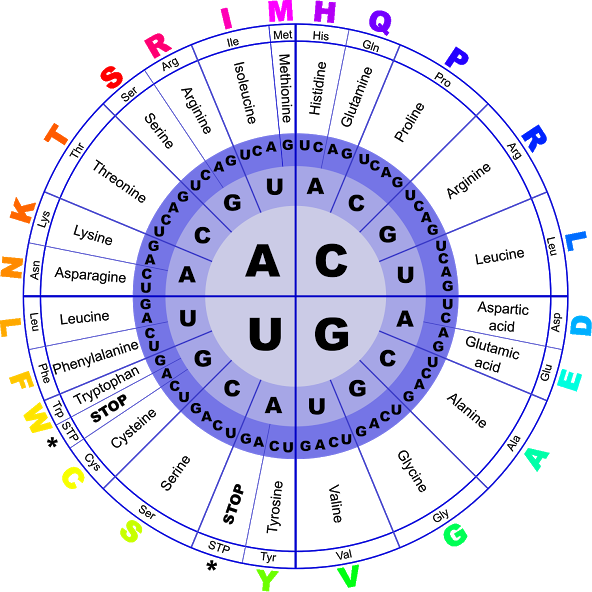
\includegraphics[width=0.5\linewidth]{./figures/ch1/codon_table_circle}}
    \caption[Tableau de correspondance des triplets d'acides nucléiques et les acides aminés.]{\it Tableau de correspondance des triplets d'acides nucléiques et les acides aminés pour lesquels ils codent. <<Initiation>> désigne les codons pouvant être retrouvés comme initiateur de la traduction, <<Stop>> désignent les codons responsables de l'arrêt du processus de traduction par le ribosome.}
    \label{Fig:codon_table}
  \hspace{0.2cm}
\end{figure}


\subsubsection{La traduction, de l'ARN à la protéine}

% L'étape suivante, la traduction, débute lorsque l'ARN messager rencontre les acteurs moléculaires responsables de la traduction, les ribosomes. L'ARN  messager se lie alors aux ribosomes et l'information portée par l'ARN, copie partielle de l'information génétique initialement portée par l'ADN, est lue pour construire de nouveaux édifices moléculaires fonctionnels de la cellules, les protéines.

% Les règles qui régissent la production de protéines à partir de la lecture de l'information génétique sont décrites dans le code génétique universel, commun à tous les organismes vivants.

Lorsque l'ARNm a rejoint le cytoplasme, l'étape de traduction peut commencer. La première phase de la traduction est la reconnaissance par la sous-partie du ribosome (30S chez les bactéries, 40S chez les eucaryotes) de la région en amont de l'ARNm. Cette reconnaissance entraîne le parcours de l'ARNm par le ribosome jusqu'au codon d'initiation qui est le premier triplet de nucléotide qui sera traduit. Chaque triplet de nucléotide code pour un acide aminé particulier. Puisqu'il existe 4 nucléotides différents, 64 combinaisons de triplets sont possibles et en moyenne, un acide aminé est codé par 3 combinaisons de triplets de nucléotides différents, c'est le caractère redondant du code génétique, comme illustré dans la Figure \ref{Fig:codon_table}.
Le premier triplet de la chaîne d'ARNm et la petite sous-unité du ribosome vont alors recruter le premier ARN de transfert (ARNt, chargé de se lier aux acides aminés) ayant formé un complexe avec une méthionine et la grande sous-partie du ribosome (50S chez les bactéries, 60S chez les eucaryotes). À la suite de cette étape de reconnaissance, la construction du reste de la protéine est initiée et se caractérise par la lecture séquentielle des triplets de nucléotides de l'ARNm par le ribosome. Le ribosome fait l'interface entre l'ARNm et les complexes ARNt complémentaires/acide aminé. Les acides aminés sont liés entre eux de façon séquentielle jusqu'à ce qu'un triplet codant pour un codon-STOP (ou d'arrêt) soit atteint par le ribosome. À ce moment-là, le ribosome libère la protéine et l'ARNm et l'étape de traduction se termine. À ce moment-là, la protéine n'est pas encore fonctionnelle et doit encore subir des modifications post-traductionnelles afin de pouvoir remplir sa fonction. Un schéma simplifié de la transcription et de la traduction est illustré dans la Figure \ref{Fig:transc_trad_HD}

\begin{figure}[htb]
  \centering
  {\includegraphics[width=1.0\linewidth]{./figures/ch1/transc_trad_HD.pdf}}
    \caption[Schéma simplifié des étapes de transcription et de traduction.]{\it Schéma simplifié des étapes de transcription et de traduction. On peut voir que l'information génétique portée par l'ADN double-brin sous forme de séquences de triplets d'acides nucléiques est copiée en l'ARNm pour pouvoir traverser la membrane nucléaire et rejoindre un ribosome qui fera l'interface entre les codons de nucléotides et les acides aminés correspondants portés par les ARNt. Source : NIGMS\footnote{\url{http://images.nigms.nih.gov/index.cfm?event=viewDetail&imageID=2549}}}
    \label{Fig:transc_trad_HD}
  % \hspace{0.2cm}
\end{figure}

\subsubsection{Maturation et acquisition de la fonction protéique}

Afin de permettre leur stabilité au sein de la cellule, de les guider vers leur lieu d'action ou simplement d'assurer leur efficacité fonctionnelle, les protéines subissent plusieurs modifications post-traductionnelles dont la nature et le nombre dépendent de la nature des protéines. Ces modifications peuvent intervenir aux deux extrémités des protéines ou bien au niveau des acides aminés individuellement. Parmi les modifications post-traductionnelles, on retrouve l'ajout de groupes fonctionnels à certains acides aminés modifiant leurs propriétés, des étapes de clivage peuvent également intervenir afin d'éliminer des parties de la protéine qui étaient importantes lors des étapes précédentes, mais inutiles pour sa fonction finale. De la même façon, certaines modifications, effectuées par des molécules dites \textit{chaperonnes} ont pour rôle de donner à la protéine sa structure tertiaire finale et donc fonctionnelle. C'est le processus spécifique du \textbf{\textit{folding}} (ou \textbf{repliement}) moléculaire de la protéine. Enfin, certaines modifications permettent le bon signalement cellulaire de la protéine, à savoir le codage lui permettant de rejoindre son lieu d'action.

\section{Méthodes et outils de la biologie structurale}

La majorité des protéines ne peut pas être fonctionnelle sans structure 3d, car leur fonction découle de cette structure, en particulier de ses propriétés biomécaniques et biophysiques conditionnant des interactions avec des molécules partenaires. C'est la raison pour laquelle la biologie structurale accorde une importance primordiale à la structure, élément central dans la caractérisation de la fonction des protéines.

\begin{figure}[h]
  \centering
  {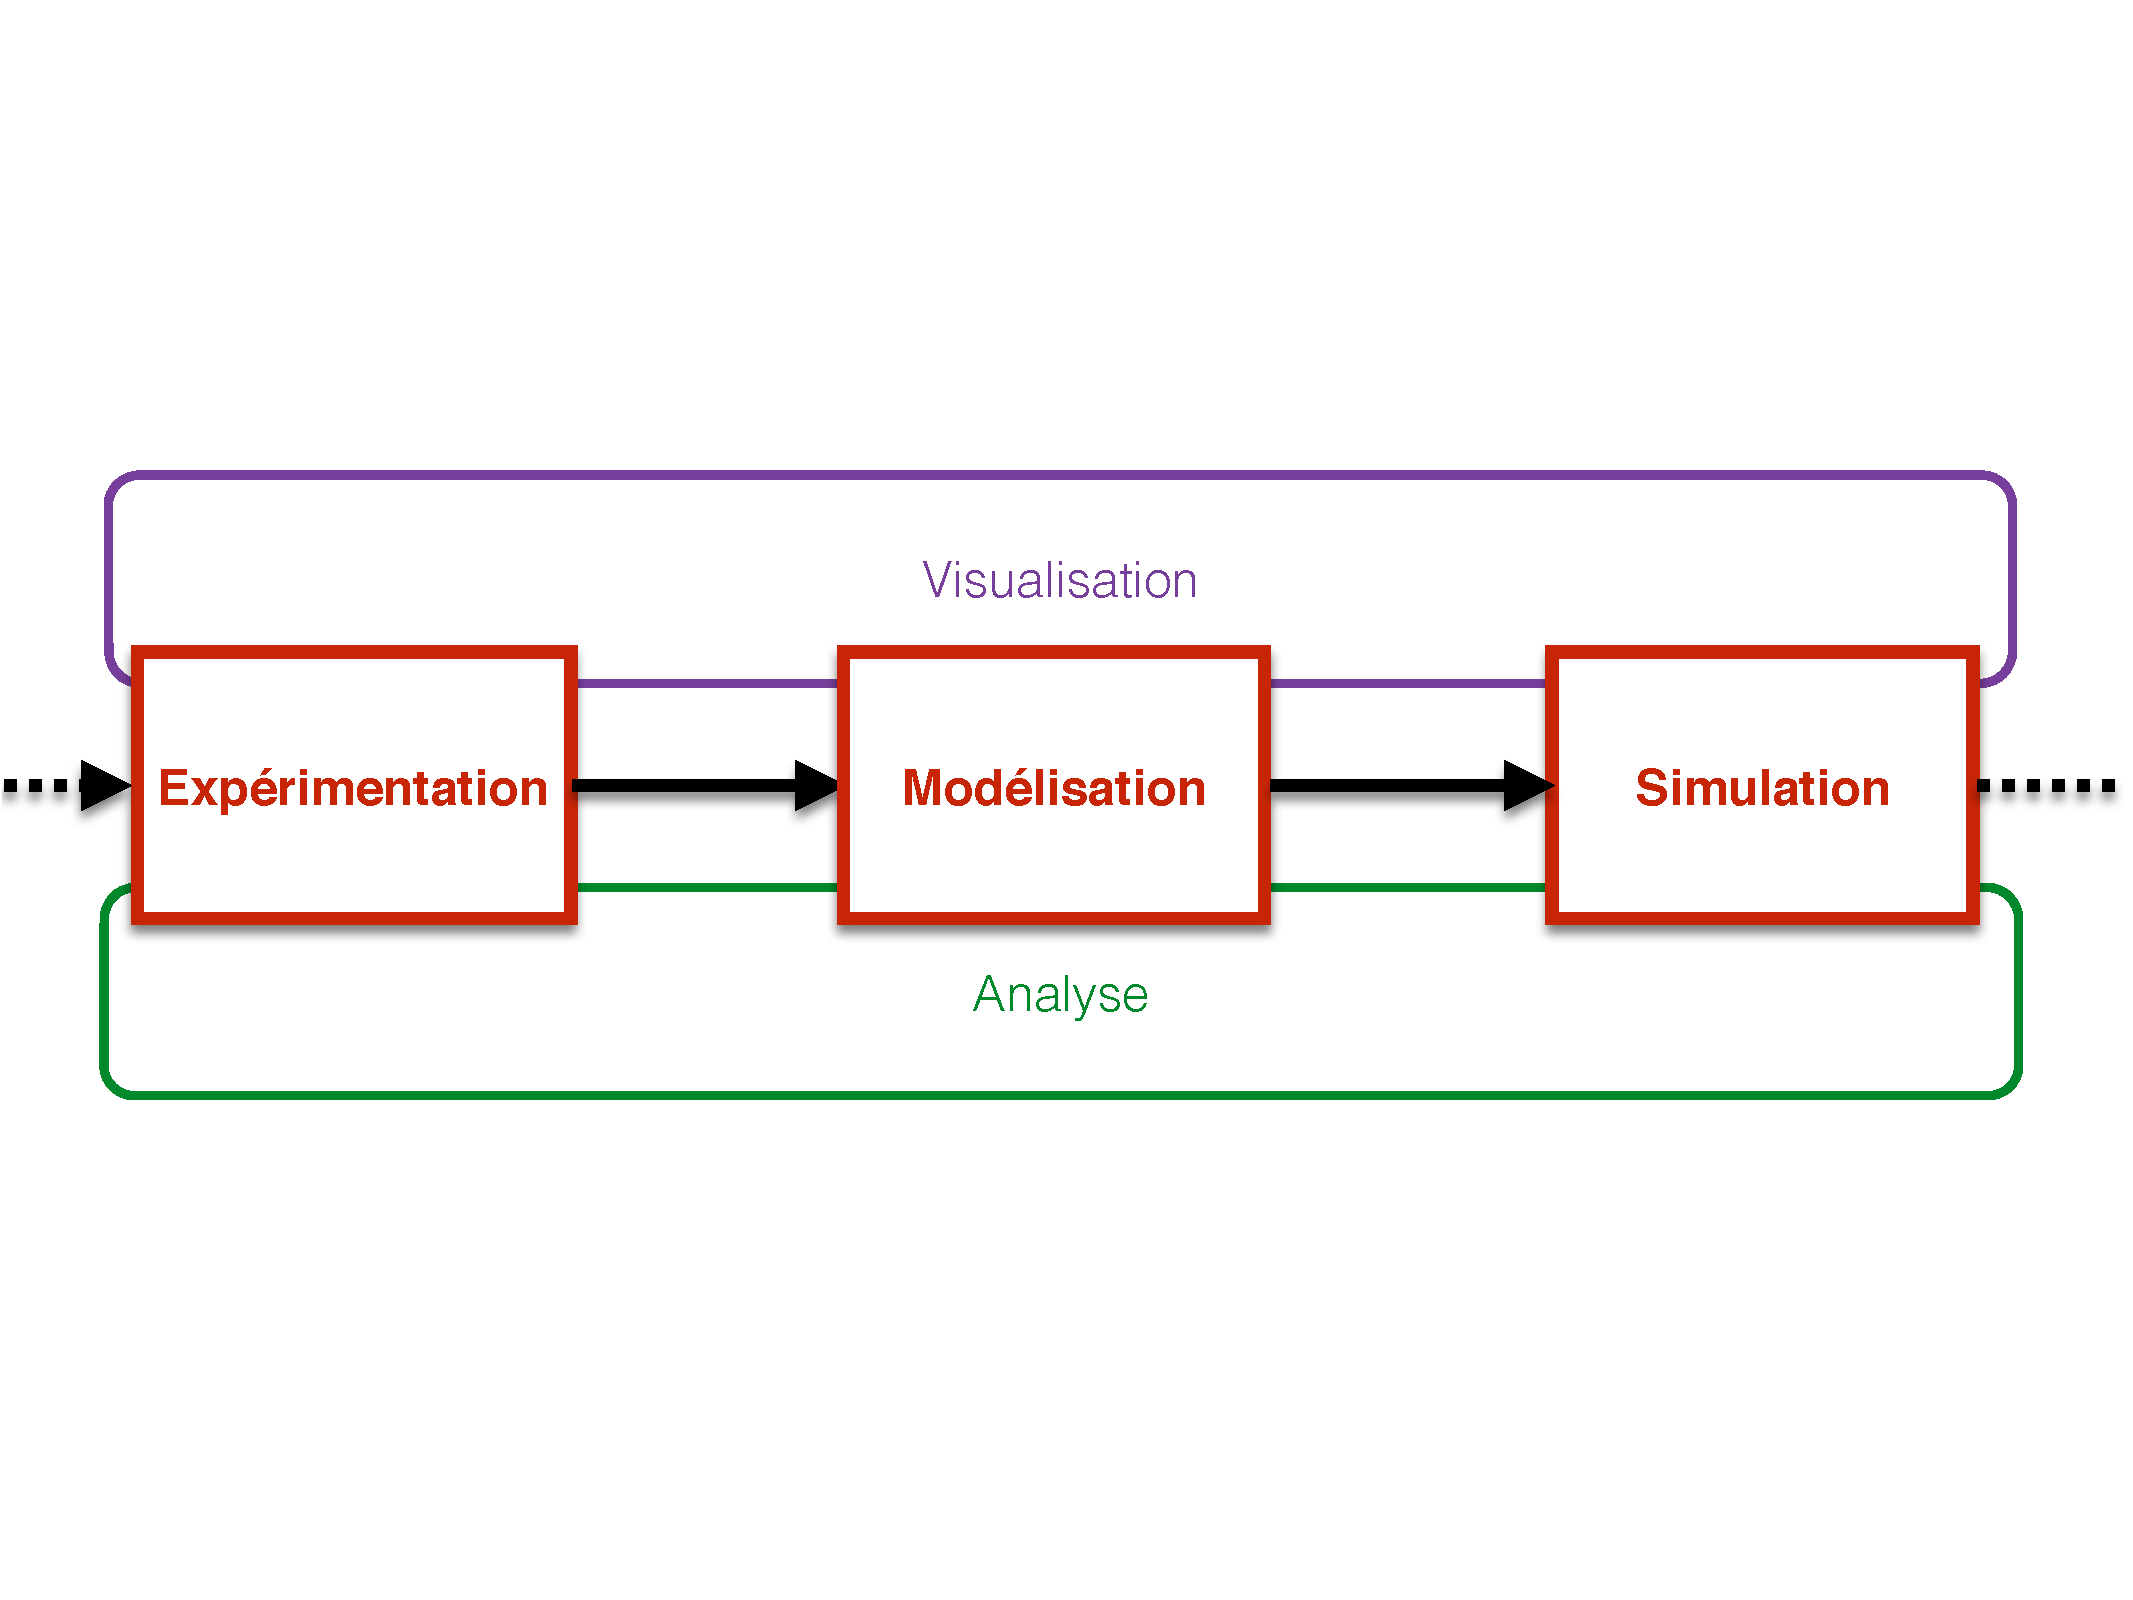
\includegraphics[width=\linewidth]{./figures/ch1/process_bio_struct_XP}}
    \caption[Schéma du processus itératif d'étude d'une structure moléculaire en biologie structurale.]{\it Les différentes étapes de l'étude d'un système moléculaire en biologie structurale.}
  \label{Fig:schema_seq_bio_struct_XP}
  \hspace{0.2cm}
\end{figure}

Il est possible de diviser le processus d'étude de la biologie structurale en plusieurs étapes distinctes mais néanmoins étroitement liées.
La Figure \ref{Fig:schema_seq_bio_struct_XP} donne un aperçu de ce découpage et identifie 3 grandes tâches : la collecte d'informations structurelles via des techniques expérimentales et théoriques, la modélisation de structures à partir des informations récoltées et la simulation moléculaire qui permet d'ajouter une dimension dynamique indispensable pour l'étude de phénomènes et enfin l'analyse et l'interprétation de résultats permettent de postuler des hypothèses quant aux phénomènes étudiés et d'affiner les étapes de modélisation.
Ces étapes ne mettent pas en jeu les mêmes outils et méthodes. Nous nous concentrerons dans cette section sur la collecte de données aboutissant à l'obtention de structures 3d.

Les protéines sont des unités biologiques de taille microscopique, leur taille oscillant entre quelques dizaines et quelques centaines d'Angströms (\r{A} = \SI{e-10}{\metre}) et donc invisibles pour des systèmes de photographies standards. En effet, les techniques de microscopie optique ne peuvent permettre aujourd'hui une observation à l'échelle atomique, quel que soit l'objet d'étude. Notons que cette taille en Angströms est indicative et inappropriée pour désigner la grosseur des protéines. On préfère utiliser le kiloDalton (kDa) qui est une mesure de masse, 1 Da correspondant à la masse d'un atome d'hydrogène. Un acide aminé représente environ 110 Da et une protéine entre 15 et plusieurs millions de kDa pour les complexes multimériques les plus importants.

L'ensemble des approches expérimentales et théoriques permettant d'étudier la structure des protéines peut être divisé en 3 grandes approches : les \textbf{techniques expérimentales}, regroupant les techniques utilisant des extraits naturels des protéines étudiées et cherchant à obtenir leur structuration par des outils de mesure \textit{in vitro}. Les approches de \textbf{modélisation/simulation} mettent en place des modèles informatiques de structures 3d à partir d'informations physico-chimiques et/ou statistiques utilisés comme paramètres de logiciels de calcul. Enfin, les programmes de \textbf{visualisation moléculaire} vont permettre d'observer et d'analyser les structures obtenues à partir des deux approches précédentes grâce à des codes graphiques précis dans le but d'extraire, d'illustrer ou de communiquer de nouvelles connaissances scientifiques.

\subsection{Expérimentations}

La nature des protéines et l'environnement dans lequel elles sont naturellement structurées impliquent l'utilisation de techniques expérimentales devant à la fois préserver leur nature et ne pas les dégrader ou les détruire, mais également assurer une précision minimum pour extraire des informations structurales et géométriques qui seront utilisées pour la caractérisation de leur fonction.
Les techniques expérimentales utilisées en biologie structurale pour obtenir la structure tridimensionnelles de biomolécules sont coûteuses en raison de leur complexité. Ce sont des méthodes physiques indirectes qui sont principalement utilisées afin d'obtenir des informations sur la structure 3d d'une biomolécule à l'échelle atomique. La plupart de ces techniques mettent en jeu des instruments de mesure de haute technologie et demandent souvent une préparation complexe et longue de l'échantillon pour qu'il soit suffisamment concentré en protéines. Il nécessitent également des conditions de stockage adaptées et dépendantes de la technique utilisée.

\subsubsection{Cristallographie à rayons X ou radiocristallographie}

Parmi ces techniques expérimentales, la plus ancienne et la plus utilisée, principalement pour sa précision, est la cristallographie aux rayons X ou radiocristallographie. Cette technique consiste à envoyer un faisceau de rayons X sur un cristal composé exclusivement de la biomolécule étudiée. La mesure des angles et de l'intensité des rayons réfractés permet d'obtenir une image tridimensionnelle de la densité électronique dans le cristal. À partir de cette densité, il est possible d'obtenir la position moyenne des atomes présents dans le cristal ainsi que les liens existants entre eux en superposant la séquence d'atomes, connue, dans la carte de densité électronique ainsi obtenue. Le processus est schématisé dans la Figure \ref{Fig:cristallographie_x_ray}.

\begin{figure}[htb]
  \centering
  {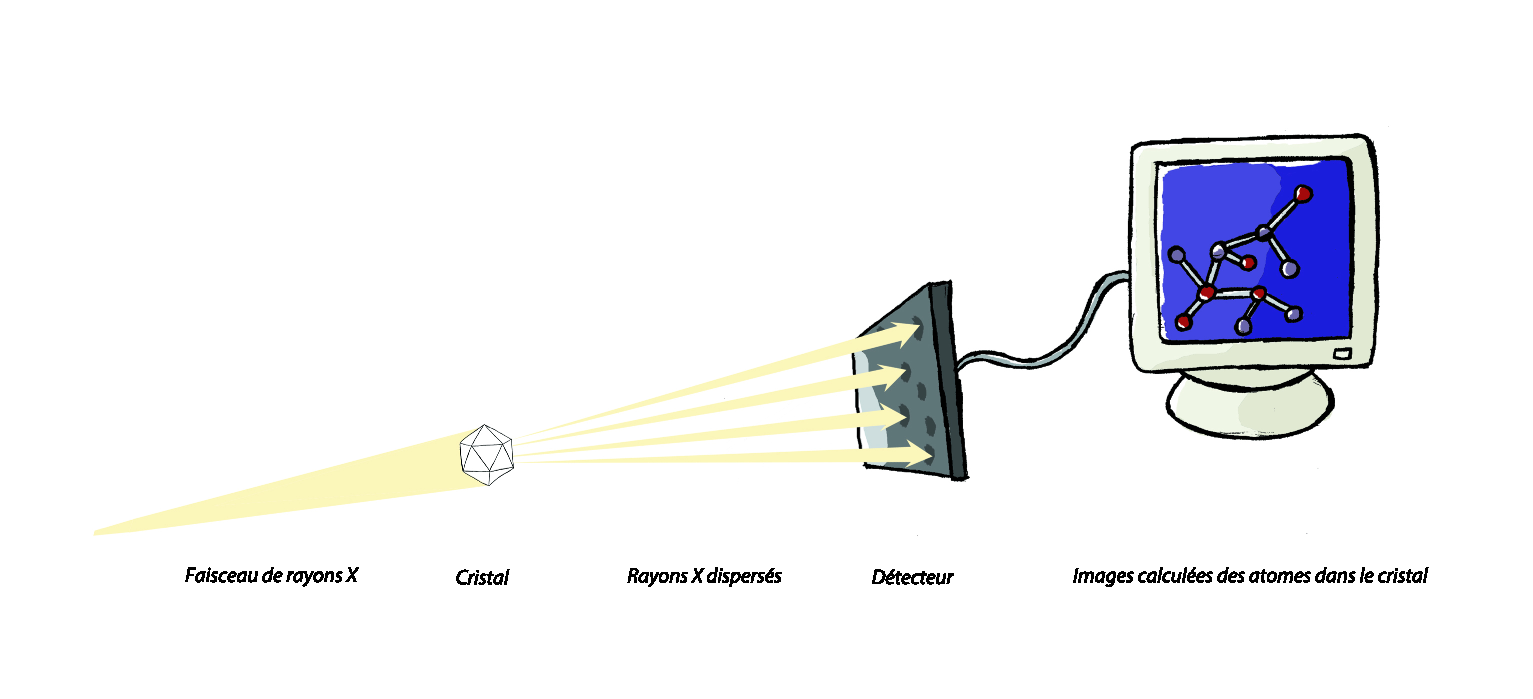
\includegraphics[width=0.9\linewidth]{./figures/ch1/cristallographie_x_ray.pdf}}
    \caption[Schéma simplifié de la cristallographie à rayons X.]{\it Schéma simplifié de la cristallographie à rayons X où les rayons X traversent un échantillon cristallisé avant d'être dispersés et capturés par un détecteur avant d'être interprétés informatiquement. Source : NIGMS\footnote{\url{http://images.nigms.nih.gov/index.cfm?event=viewDetail&imageID=2512}}}
    \label{Fig:cristallographie_x_ray}
  \hspace{0.2cm}
\end{figure}

L'avantage de la radiocristallographie est sa très grande précision et l'absence de limite de taille pour le cristal, permettant l'observation de structures moléculaires de très grande taille comme les ribosomes (environ un million d'atomes). 
Suivant les biomolécules observées, il est possible d'obtenir des structures tridimensionnelles à des résolutions minimales en dessous de 1\r{A} pour une précision sur la position des atomes à moins de 0.5\r{A}. 1\r{A} constituant une précision atomique. Les cartes de densité et les modèles atomiques créés à partir de ces cartes sont illustrés dans la Figure \ref{Fig:resolution_xray}.

Certaines biomolécules sont néanmoins très difficiles à cristalliser et on évalue à environ un quart la proportion de macromolécules permettant de créer un cristal de taille et de qualité suffisante de diffracter suffisamment les rayons X. Cette cristallisation est une étape difficilement automatisable et qui se révèle majoritairement empirique, demandant un travail de préparation spécifique en plus de l'application de la technique. Les hydrogènes présents dans les macromolécules sont très difficiles à percevoir du fait de leur très faible densité électronique. L'obtention d'une structure 3d par radiocristallographie est fastidieuse et nécessite en moyenne plusieurs mois de travail.

\begin{figure}[htb]
  \centering
  {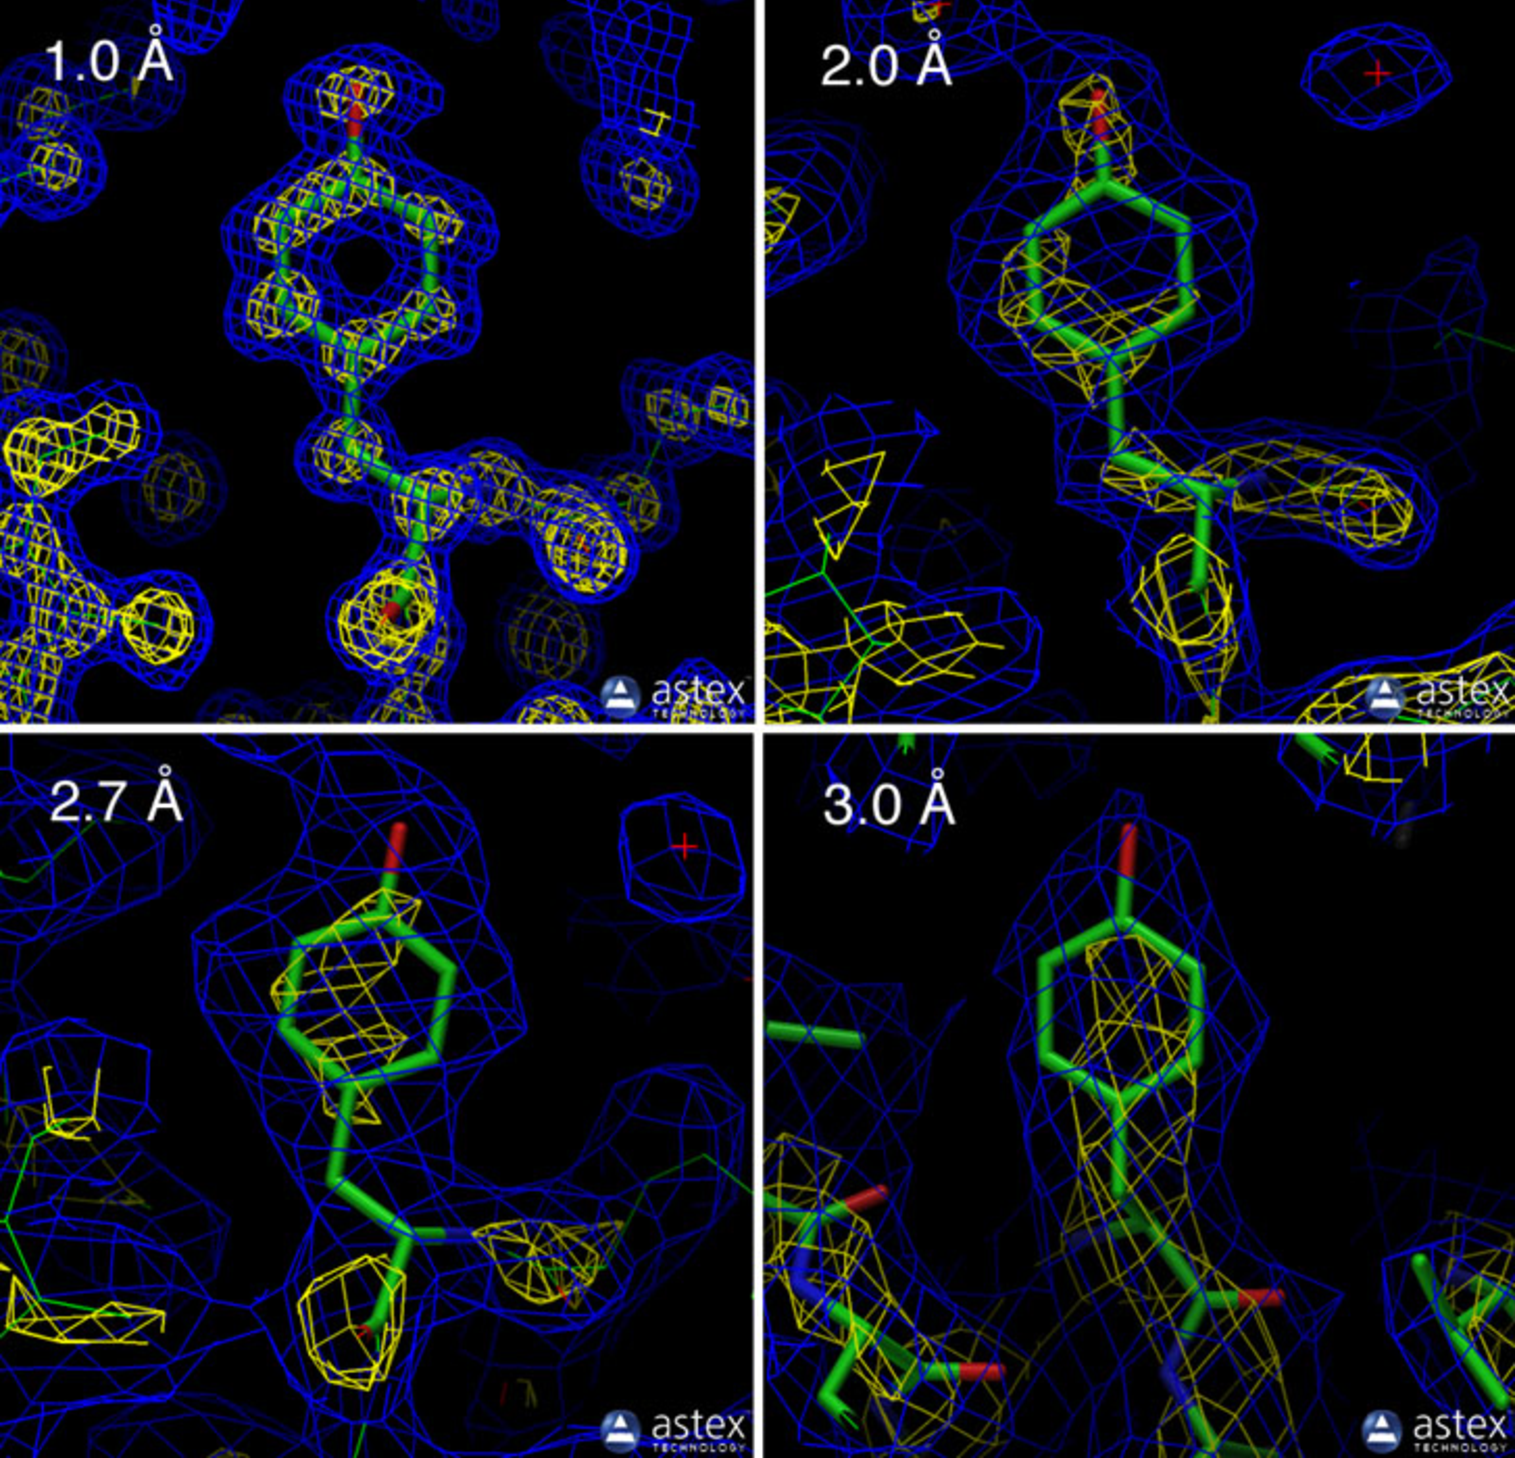
\includegraphics[width=0.5\linewidth]{./figures/ch1/resolution_xray.pdf}}
    \caption[Rendu graphique d'un acide aminé et de sa carte de densité obtenue par cristallographie.]{\it Rendu graphique d'un acide aminé représenté par des bâtonnets verts et rouges au sein de sa carte de densité obtenu par cristallographie et représentée par un mesh de triangles bleus. Les différentes parties de l'image correspondent à des cartes de densité électronique à différentes précisions. Source : RCSB\footnote{\url{http://www.rcsb.org/pdb/101/static101.do?p=education_discussion/Looking-at-Structures/resolution.html}}}
    \label{Fig:resolution_xray}
  \hspace{0.2cm}
\end{figure}


La cristallographie nécessite également d'observer les protéines dans un environnement non naturel, le cristal, dont la protéine est le seul composant. Elle se déroule en plus à basse température et ne reflète qu'un état unique de la protéine à cette température. Il n'est donc pas possible d'observer de dynamique structurelle. Enfin, même s'il est possible d'observer des complexes moléculaires de grande taille, la résolution obtenue est souvent moindre que celle des protéines composées d'entre 100 et 1000 acides aminés.

% \commentaire{MB: me manquent les principales limitations de la xtallo; e.g. environnement non-naturel; basse temperature; pas de dynamique; facteurs B..}


\subsubsection{Spectroscopie à Résonance Magnétique Nucléaire - RMN}

Également très utilisée, la Spectroscopie à Résonance Magnétique Nucléaire ou RMN consiste à envoyer une séquence d'impulsions électromagnétiques sur une molécule en présence d'un champ magnétique \cite{wuthrich1986nmr}. La fréquence et la séquence des impulsions électromagnétiques sont propres à chaque type d'atome. Cette technique se base sur les mouvements de rotation naturels des atomes, créant un mini champ magnétique (ou spin). Seuls quelques atomes sont détectables en spectroscopie RMN, car ils possèdent un spin nucléaire particulier de 1/2. En biologie structurale, c'est principalement le proton H\textsuperscript{1} qui est ciblé. Les noyaux atomiques possédant des spins sont excités par les impulsions électromagnétiques et absorbent l'énergie ainsi reçue. Lors de l'étape de relaxation suivant l'impulsion, les noyaux atomiques relâchent de l'énergie sous forme de résonance à différentes longueurs d'onde, calculée et reportée par les instruments de mesure (cf. Figure \ref{Fig:rmn}). Cette résonance varie en fonction de la nature de l'atome excité et de son environnement. Il est donc possible, grâce à ces résonances, pour un atome donné, d'avoir des informations sur la nature et le nombre d'atomes voisins, la liaison chimique dans laquelle il est impliqué, sa distance à d'autres atomes, sa mobilité, etc. À la différence de la cristallographie où la protéine est cristallisée, la RMN peut s'appliquer sur une molécule solubilisée (mise en solution liquide). Il est de fait plus aisé de préserver la structure et la fonctionnalité d'une molécule en solution que sous forme de cristal. 

\begin{figure}[htb]
  \centering
  {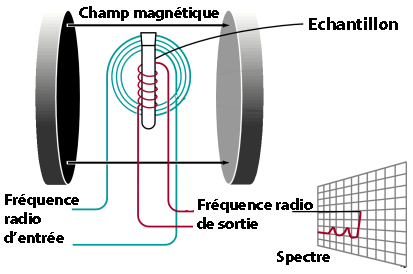
\includegraphics[width=0.55\linewidth]{./figures/ch1/rmn.png}}
    \caption[Schéma de la technique de spectroscopie RMN.]{\it Schéma de la technique de spectroscopie RMN. Un échantillon est placé dans un champ magnétique et excité par des impulsions radio successives. La relaxation des atomes de l'échantillon induisent un signal radio interprété par puissance de signal sur un spectre.}
    \label{Fig:rmn}
  \hspace{0.2cm}
\end{figure}

Il est également possible d'avoir des informations sur la dynamique de la molécule puisqu'au contraire de quand elle se trouve dans un cristal, une molécule en solution n'est pas statique.
L'état dynamique de la molécule est aussi un inconvénient pour obtenir une structure 3d fixe puisque la précision de la mesure sera perturbée par les changements structurels de la molécule. L'un des autres inconvénients de la spectroscopie RMN est la limitation en taille des molécules, observée du fait de la complexité du traitement des signaux de résonance magnétique, ces derniers se superposant tous sur un spectre borné dont les limites ne varient pas avec la complexité de la protéine étudiée. Ainsi, plus le nombre d'atomes est important, plus le nombre de signaux augmentera et s'accumulera sur un spectre de largeur constante. La taille optimale pour la RMN varie entre 10 et 50 kilodaltons (kDa) correspondant à des molécules de 1.500 à 10.000 atomes. De plus, pour les plus grosses molécules, il est nécessaire d'effectuer un marquage isotopique permettant d'obtenir un spectre non plus 2d, mais 3d où les atomes ciblés, en plus de H\textsuperscript{1}, sont le C\textsuperscript{13} et le N\textsuperscript{15} après enrichissement spécifique de la biomolécule observée.


\subsubsection{Cryo-microscopie électronique - Cryo-EM}

\begin{figure}[htb]
  \begin{subfigure}{.4\textwidth}
  \centering
  {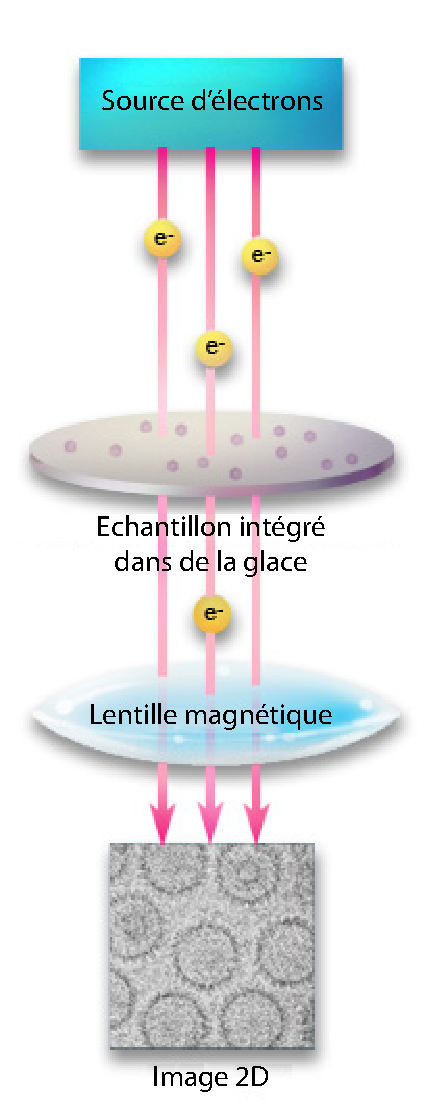
\includegraphics[height=10cm]{./figures/ch1/cryoem.pdf}}
    \caption{}
    \label{Fig:cryoem}
  \end{subfigure}
  \begin{subfigure}{.6\textwidth}
  \centering
  {\includegraphics[height=10cm]{./figures/ch1/cryoem_density.png}}
  \caption{}
    \label{Fig:cryoem_density}
  \end{subfigure}
  \caption[(a) Schéma illustrant la technique de cryo-microscopie électronique. (b) Carte de densité électronique d'un complexe protéique.]{\it (a) Schéma illustrant la technique de cryo-microscopie électronique\footnote{\url{http://www.eicn.ucla.edu/cryoem}}. Les électrons traversent l'échantillon prisonnier de la glace avant d'atteindre une lentille magnétique qui va les modifier et les projeter sur un scintillateur permettant d'obtenir une image de la projection.
  (b) Carte de densité (en rendu surfacique transparent blanc) d'un complexe protéique (GroEL-GroES) composé de multiples sous-unités de la famille des protéines chaperonnes. Source : \cite{hoang2013gemfitter}}
\end{figure}

Une autre technique plus récente en biologie structurale, la Cryo-microscopie électronique (Cryo-EM), consiste à utiliser le principe de la microscopie électronique, et donc d'utiliser un faisceau de particules d'électrons au lieu de rayonnements électromagnétiques (lumière) comme en microscopie optique, sur un échantillon préalablement cryogénisé lors de l'étape de fixation. Le faisceau de particules d'électrons passe au travers de lentilles électrostatiques et électromagnétiques puis au travers de l'échantillon cryogénisé où il est modifié pour former une image électronique finalement amplifiée par d'autres lentilles et projetée sur un scintillateur (cf. Figure \ref{Fig:cryoem}).
La protéine est ainsi visualisée sous plusieurs angles et les images générées sont ensuite traitées sur ordinateur afin de rassembler les différents points de vue et de créer une carte de densité électronique 3d rapportant le volume global de la protéine (voir Figure \ref{Fig:cryoem_density}).

La particularité de la cryofixation de l'échantillon, par opposition à la fixation chimique ou la déshydratation, est que l'échantillon est amené très rapidement à la température de l'azote liquide (\SI{-195.79}{\degreeCelsius}) ou de l'hélium liquide (\SI{-269}{\degreeCelsius}) afin que la glace formée ne soit pas cristalline et que le spécimen étudié conserve son état naturel. Pour des biomolécules, cela assure une conservation d'une structure 3d stable de la molécule. La cryo-EM permet d'étudier des structures moléculaires de grandes tailles, à partir de 300kDa jusqu'à des tissus de plusieurs centaines de nanomètres, en passant par les ribosomes, les virus ou les composants cellulaires.

Bien qu'en constant développement, la cryo-EM possède une résolution relativement faible comparée aux deux techniques précédentes puisque les cartes de densité obtenues par cette technique ne permettent pas une résolution de moins de 4\r{A} pour les cartes les plus précises\cite{zhou_atomic_2011}. L'exposition de l'échantillon à un faisceau de particules d'électrons, combinée à sa cryogénisation, dommage significativement l'échantillon qui ne peut être réutilisé ensuite.



\subsubsection{Diffusion des rayons X - SAXS}

La technique SAXS est basée sur les interactions élastiques entre les photons et les nuages électroniques \cite{guimer1955small}. Cette technique s'inspire directement de la diffraction des rayons X quand ils traversent un cristal (diffraction de Bragg) entraînant la diffusion de ces rayons à différents angles de l'ordre de la dizaine de degrés. L'angle de diffraction est inversement proportionnel à la distance interatomique des atomes présents dans le cristal. Or, les informations nécessaires pour constituer la structure 3d de macromolécules concernent des distances trop grandes pour que les angles de diffraction soient facilement détectables. La gamme d'angles pouvant être mesurés permet de rapporter des distances d'au minimum quelques nanomètres (environ 10\r{A} de résolution). Il est nécessaire d'utiliser un rayonnement X monochromatique très proche de l'échantillon constitué de la biomolécule d'intérêt. De la même manière que pour les précédentes techniques, une carte de densité, ici densité électronique, est ainsi générée après interprétation des angles de diffraction calculés par l'instrument de mesure placé à la suite du faisceau émis à travers l'échantillon. (voir Figure \ref{Fig:saxs}).

\begin{figure}[htb]
  \centering
  {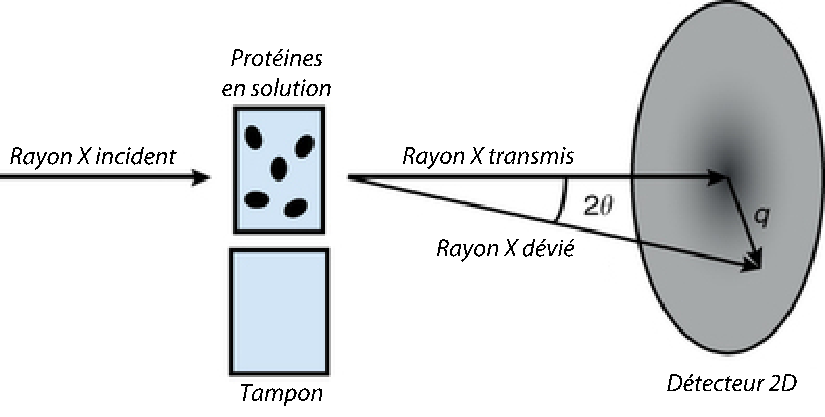
\includegraphics[width=0.6\linewidth]{./figures/ch1/saxs.pdf}}
    \caption[Schéma de la technique de diffusion des rayons X - SAXS.]{\it Schéma simplifié illustrant la technique de diffusion des rayons X. Ces rayons sont projetés au travers d'un échantillon et sont légèrement déviés par celui-ci puis capturés par un détecteur 2d. L'angle de déviation mettra en avant les distances interatomiques de plusieurs nanomètres. Source : \cite{skou2014synchrotron}}
    \label{Fig:saxs}
\end{figure}

L'un des avantages de la technique SAXS par rapport à la cristallographie est l'absence de cristal pour effectuer l'expérience, l'échantillon étant mis en solution. Mais cet avantage est terni par la résolution de la technique qui ne permet pas d'obtenir une description atomique d'une biomolécule. Elle est souvent utilisée pour obtenir une structure 3d approximative de complexes moléculaires ou de composants cellulaires de grandes tailles grâce à une étape d'assemblage où la représentation atomique des composants individuels de ces complexes sont intégrés dans une carte de densité. Une de ces forces repose aussi sur la rapidité de l'expérience qui, en combinant l'ensemble des étapes de préparation, expérimentation et analyses des résultats, peut générer une carte de densité en quelques jours.

L'ensemble de ces techniques possède une étape d'interprétation de signal basée sur des méthodes informatiques, autrement impossible à interpréter par un être humain. La complexité de l'interprétation d'un signal provient à la fois du bruit propre au signal, majoritairement dû à la complexité des échantillons observés aujourd'hui, et du nombre de signaux, corrélé directement à la taille des protéines étudiées. L'outil informatique joue donc un rôle très important dans les processus dits expérimentaux mais ne se cantonne pas à de simples interprétations de résultats et permet également de générer des structures 3d grâce à des méthodes qui seront exposées ci-après (voir section \ref{model_simu}).




\subsubsection{Banques de structures protéiques} \label{protein_DB}

Les bases de données biologiques permettent de regrouper l'ensemble des informations scientifiques obtenues au cours de l'histoire et les mettre à disposition de la communauté scientifique. Les bases de données structurales regroupent plus particulièrement des structures obtenues par techniques expérimentales dont il est possible d'obtenir la représentation 3d sous forme de fichier informatique. 
Elles voient de plus en plus leur intégration au sein de portails biologiques gérant la conformité des données aux standards du domaine, leur accès à l'ensemble des scientifiques et éventuellement leur association avec des données d'autres domaines scientifiques proches.

L'une des bases de données les plus utilisées en biologie structurale est la \textbf{Protein Data Bank} (PDB) \cite{berman_protein_2000} qui regroupe l'ensemble des structures 3d de protéines publiées et vérifiées dans plusieurs formats standards, formats utilisés en entrée de la majorité des outils de bio-informatique structurale. Les structures 3d présentes dans la PDB proviennent majoritairement de cristallographie rayon X ou de spectroscopie RMN (89\% pour la cristallographie, 10\% pour la RMN). Aujourd'hui, environ 105 000 structures de protéines, 5 200 structures de complexes mixtes protéine/acide nucléique et 2 800 structures d'acides nucléiques ont été déposé dans la PDB.

On peut également noter d'autres banques de données de structures protéiques :
\begin{itemize}
  \item \textbf{SCOP} (Structural Classification of Proteins)\footnote{\url{http://scop.berkeley.edu/}} est une banque de données regroupant les protéines de la PDB présentant une relation de similarité structurale et d'évolution \cite{murzin1995scop}. Les structures sont ainsi regroupées en 3 niveaux hiérarchiques : famille, superfamille et repliement.
  \item \textbf{CATH} (Class Architexture Topology and Homology)\footnote{\url{http://www.cathdb.info/}} regroupe les protéines dont la structure a été déterminée par RMN ou par cristallographie avec une résolution de détermination supérieure à 3\r{A} \cite{sillitoe2015cath}. Elle est composée de 4 niveaux hiérarchiques basés sur la structure des protéines, du plus générique au plus précis : classe, architecture, topologie et superfamilles homologues.
  \item \textbf{FSSP} (Fold Classification based on Structure-Structure alignement of Proteins)\footnote{\url{http://protein.hbu.cn/fssp/ekhidna.biocenter.helsinki.fi/dali/start.html}} regroupe les structures représentatives de la PDB \cite{holm1996mapping}. Elle filtre les protéines dont les structures sont considérées comme redondantes dans la PDB, avec plus de 25\% d'identité au niveau des séquences et de la structure après une comparaison des séquences et des motifs structuraux les composant. Elle se base sur le programme DALI d'alignement structural, consistant à comparer l’enchaînement des motifs structuraux entre les protéines, pour obtenir ces structures non redondantes \cite{holm1998touring}.
  \item \textbf{MMDB} (Molecular Modeling Database)\footnote{\url{http://www.ncbi.nlm.nih.gov/structure/}} est un sous-ensemble de la PDB excluant les modèles théoriques \cite{madej2014mmdb}. Elle héberge des données structurelles conventionnelles mais non figées et pouvant être enrichies en ajoutant d'autres informations structurelles complémentaires obtenues par des technologies comme la microscopie électronique.
\end{itemize}

Parmi les informations stockées dans des bases de données et utilisées en biologie structurale en dehors de données purement structurales on retrouve : les profils biologiques des protéines avec leur structure primaire/secondaire/tertiaire, leur environnement cellulaire, leur rôle, etc. (SWISSPROT+TrEMBL \cite{boeckmann2003swiss}, PDB, etc.); les réseaux d'interactions moléculaires (interactome) mettant en avant les partenaires moléculaires déjà identifiés (STRING \cite{Snel15092000}, CCSB Interactome Database \footnote{\url{http://interactome.dfci.harvard.edu/}}, etc.); les évolutions génomiques des séquences d'ADN codantes identifiant les régions évoluant rapidement au sein des protéines (séquence primaire changeante) et les régions plus stables et donc potentiellement importantes pour la fonction métabolique de la protéine (USCS \cite{kent2002human}, Ensembl \cite{hubbard2002ensembl}, etc.). 


\subsection{Modélisation et simulation} \label{model_simu}

Comme il n'est pas possible expérimentalement de filmer une protéine dans son environnement, en complément des techniques expérimentales, il est nécessaire d'utiliser des approches computationnelles, notamment pour accéder aux propriétés dynamiques et mécaniques des protéines. Il s'agit aussi de compléter les informations structurelles recherchées ou de générer des modèles pour des protéines dont la nature empêche leur étude expérimentale (mauvaise solubilité, instabilité en solution, dégradation par les rayons X, etc.). Ces approches dites \textit{in silico} sont moins coûteuses que les approches expérimentales, mais ont parfois un facteur de confiance légèrement moins important que les approches énoncées précédemment car elles dépendent uniquement d'un set de paramètres pour générer des modèles structuraux. Les approches computationnelles ont cependant beaucoup évolué ces deux dernières décennies, portées par l'essor de l'informatique. Elles intègrent des paramètres physico-chimiques de plus en plus précis permettant de modéliser des structures 3d avec de plus en plus de précisions. Leurs limitations actuelles se situent davantage au niveau du temps de simulation qui doit respecter un rapport étroit entre le temps nécessaire pour l'observation d'un phénomène biologique et le temps alloué aux experts pour leurs expérimentations \cite{shaw2010atomic}. De la même manière, la nature différente des protéines et de leur environnement nécessite un réglage précis des paramètres utilisés au sein de ces techniques. 
La reconnaissance de l'apport des méthodes théoriques pour la modélisation moléculaire est d'ailleurs très présente aujourd'hui et fut mis en exergue en 2013 par l'obtention du prix Nobel de chimie par ses pionniers (Martin Kaplus, Michael Levitt et Arieh Warshel)\cite{_nobel_2013}.

La différence entre la précision des techniques expérimentales et computationnelles est donc aujourd'hui très fine et ces deux approches sont utilisées de façon complémentaires au sein de nombreuses études.

La modélisation moléculaire consiste à étudier \textit{in silico} les caractéristiques et le comportement des molécules par des techniques théoriques et computationnelles variées. Son champ d'applications regroupe les méthodes permettant d'étudier la structure, la dynamique, les propriétés de surfaces et la thermodynamique des systèmes biologiques. Parmi les activités biologiques pouvant être décrites par les outils de modélisation moléculaire, on retrouve le repliement des protéines aboutissant à leur structure 3d, les catalyses enzymatiques, la stabilité des protéines, les changements conformationnels associés aux fonctions biomoléculaires et la reconnaissance moléculaire des protéines, ADN et autres complexes membranaires.
La modélisation moléculaire regroupe entre autres les méthodes capables de générer des modèles de structures 3d de biomolécules à partir d'un ensemble de données décrivant un ensemble de connaissances. Ces données peuvent être simplement la structure primaire d'une protéine ou bien provenir d'autres résultats expérimentaux ou computationnels. Ces deux approches se basent sur des simulations de mécanique moléculaire prenant en compte des paramètres physico-chimiques ou mécaniques, prédisant l'évolution de chaque particule dans son environnement (cellulaire, extracellulaire, membranaire, etc.).

La modélisation doit faire face à l'hétérogénéité importante qui existe entre les protéines. Suivant leur taille, leur complexité et leur environnement différentes méthodes répondent à différents besoins. De la même manière, le niveau de représentation des systèmes moléculaires varie au sein des méthodes. Ces différents niveaux permettent d'obtenir un équilibre être les ressources de calcul nécessaires et la résolution demandée. Un retour sur les différentes méthodes et représentations peut être trouvé dans l'article de Marc Baaden et Richard Lavery \cite{baaden2007there}.


\subsubsection{Modèles théoriques des biomolécules}

La représentation du niveau énergétique d'une protéine peut être faite de différentes manières suivant la précision recherchée et les ressources de calcul à disposition. L'un des enjeux de la modélisation moléculaire est la recherche d'un équilibre entre une précision suffisante des modèles 3d générés et la puissance de calcul nécessaire à leur génération qui doit rester dans une échelle temporelle et économique raisonnable pour l'expert scientifique.
L'ensemble des phénomènes physico-chimiques utilisé pour simuler une structure moléculaire dans son environnement constitue un \textbf{champ de force} et permet de calculer l'énergie potentielle du système (voir section \ref{forcefield}). Comme dans la nature, la simulation cherche à minimiser cette énergie potentielle.

\myparagraph{Modèle quantique} \label{quantic}

Nous ne ferons qu'une brève description sur les modèles \textit{quantiques} biologiques du fait de leur complexité et l'impossibilité de leur application sur des systèmes moléculaires de plus de quelques centaines d'atomes. Il est cependant important de noter que les modèles quantiques sont les modèles les plus précis pour décrire un système moléculaire. Ils prennent en compte les effets quantiques du système étudiés en se plaçant à une échelle subatomique puisqu'ils intègrent les contributions énergétiques des électrons et du noyaux, constituants des atomes. Ils se basent sur l'équation de Schrödinger \cite{schrodinger1926undulatory} qui décrit le mouvement d'une particule grâce à sa masse, son énergie, la constante de Planck et son énergie potentielle. Cette équation est trop complexe pour admettre une solution analytique et est donc résolue de façon approchée et/ou numérique. L'approximation de Born-Oppenheimer \cite{born1927quantentheorie} est une première tentative pour réduire la complexité de ces résolutions en utilisant le fait que les masses des électrons sont très petites par rapport aux masses des nucléons. Elle permet la décomposition de l'équation de Schrödinger en deux étapes, mais ne suffit pas à réduire la complexité de façon assez importante pour que son application soit envisageable sur des systèmes composés de plus de quelques atomes.

Nous nous concentrerons donc sur les méthodes de modélisation utilisant des modèles dits \textit{classiques} décrivant les particules non plus à l'échelle quantique, mais à l'échelle atomique. Les calculs quantiques ne sont cependant pas laissés de côté et sont utilisés pour dériver des valeurs énergétiques moyennes décrivant les interactions entre deux ou trois particules. Ces valeurs fixes serviront de base pour les paramètres des modèles \textit{classiques}.

A la frontière des modèles quantiques et classique se situent les approches mixtes de QM/MM \cite{warshel1976theoretical}. Ces approches rassemblent au sein des simulations, la précision du modèle quantique et la rapidité du modèles classique. Elles se basent sur une définition multi-échelle de la protéine qui contiendra seulement quelques régions décrites par des équations quantiques, le reste étant décrit par un modèle classique. Les régions choisies comme décrites quantiquement correspondent à des régions d'intérêt et impliquées dans le phénomène biologique étudié.

Une autre incursion des modèles quantiques dans la biologie se retrouve dans les approches Car Parrinello \cite{car1985unified}, utilisées par exemple avec succès à l'ADN. Cette approche est une approximation de la méthode Born-Oppenheimer citée précédemment, elle maintient les électrons dans un état stable qui permet d'éviter l'utilisation de minimisation à chaque pas de temps d'une simulation.
% \commentaire{MB: je pense qu'il faut parler brievement des approches mixtes, eq QM/MM qui sont utilises en bio, par ex. pour les enzymes; a noter aussi qu'on trouve par ex. des etudes Car-Parrinello de l'ADN donc la quantique fait bien des incursions dans la bio}

\myparagraph{Modèle classique} \label{forcefield}

Les modèles classiques sont eux empiriques, découlant du modèle quantique, ils décrivent une protéine à travers les propriétés physico-chimiques des atomes la composant. L'ensemble des équations régissant l'énergie d'un système moléculaire et de ses paramètres associés est regroupé dans un \textbf{champ de force}. Cette notion de champ de force est primordiale dans le modèle classique et est utilisée par la majorité des approches de simulation. L'ensemble des contributions énergétiques décrites dans les champs de force vont permettre d'évaluer les modèles moléculaires que génèrent les calculs lors de la phase de modélisation ou de simulation.

D'un point de vue calculatoire, un champs de force est un ensemble de règles et de paramètres imposant aux particules de la protéine les lois physiques s'appliquant à l'échelle moléculaire. Ces règles peuvent inclure de nombreux paramètres comme les conditions physiques de l'environnement (température, pression, etc.) et les propriétés physiques des particules (polarité, charge, rayon, etc.). Les paramètres physiques comme la température, la pression et les paramètres de la mécanique newtonienne sont utilisés au sein de fonctions de calcul, au cours du temps et permettent donc au système d'évoluer vers différents niveaux énergétiques au cours de la simulation. La dynamique moléculaire, simulant les atomes de la biomolécule selon des lois newtoniennes, 
% \commentaire{MB: pas d'accord avec ta presentation du MC comme methode de minimisation; justement le critere de Metropolis permet d'augmenter en energie et d'echantillonner..}
et les méthodes de Monte-Carlo qui permettent d'échantillonner les configurations 3d de la protéines via des changement successifs aléatoires de la position des atomes, se reposent sur ces lois physico-chimiques décrites dans chaque champs de force (voir section \ref{simu}). 

Un champ de force est le résultat de contributions énergétiques différentes qui, combinées, vont permettre le calcul d'une énergie potentielle pour l'ensemble du système moléculaire étudié. La somme de ces contributions peut être représentée de la manière suivante :

$$E = E_{liée} + E_{nonliée}$$

où les énergies des contributions des liaisons covalentes (interactions liées), résultats de liaisons fortes entre les atomes et difficiles à défaire, et des liaisions non covalentes (interactions non liées), liaisons à longue distance énergétiquement plus faibles que les précédentes, sont données par les calculs suivants :

$$E_{liée} = E_{liaison} + E_{angle} + E_{dièdres} (+ E_{impropres})$$
$$E_{nonliée} = E_{électrostatique} + E_{vanderwaals}$$

Les paramètres influençant ces interactions regroupent les énergies de liaison entre atomes et l'énergie des angles plus ou moins complexes formés par des atomes voisins. Ils dépendent exclusivement de la configuration électronique et de la charge électrique des atomes qui varie suivant leur nature.


Les énergies de liaison et d'angle entre particules sont souvent modélisées par des potentiels harmoniques centrés autour de la valeur d'équilibre de la liaison/angle considéré et dérivés des calculs expérimentaux. Pour davantage de précision, mais à un coût computationnel plus important, on utilise parfois le potentiel de Morse qui décrit plus précisément les états vibrationnels d'une structure, car il prend en compte les effets de cassure de liaison ainsi que l'existence d'états non liés. La différence de contribution de ces deux potentiels est représentée dans la Figure \ref{Fig:harmonic_morse_potential}. Les angles dièdres possèdent eux plusieurs minimas et leur contribution énergétique ne peut donc pas être représentée par ces potentiels. Il est commun d'ajouter un terme décrivant les angles de torsion impropres afin de contraindre la géométrie de certains plans. On cherchera par exemple à forcer la planéité des cycles aromatiques de chaînes latérales.

\begin{figure}[htb]
  \centering
  {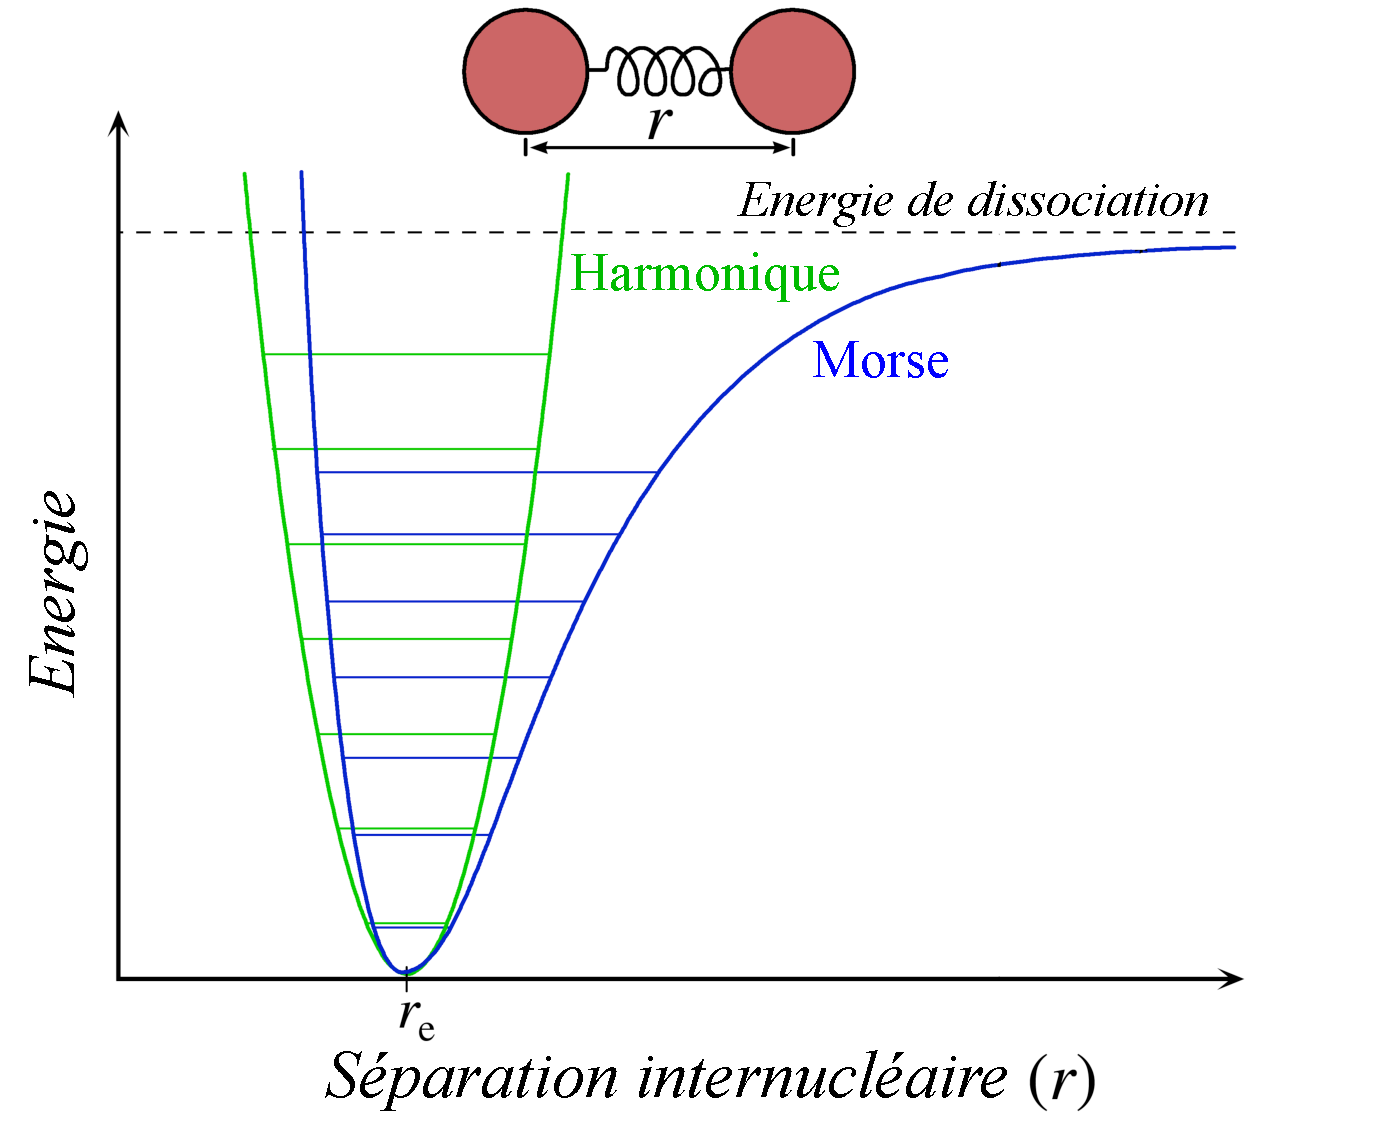
\includegraphics[width=0.6\linewidth]{./figures/ch1/harmonic_vs_morse_potential.pdf}}
    \caption[Contributions énergétiques des liaisons covalentes.]{\it Contributions énergétiques des liaisons représenté par un potentiel harmonique (en vert) ou un potentiel de Morse (en bleu) en fonction de la distance entre deux atomes. Source : \cite{assumed_graphical_2006}}
    \label{Fig:harmonic_morse_potential}
  \hspace{0.2cm}
\end{figure}

Les termes d'énergie non liée sont plus difficiles à calculer, car chaque atome interagit de façon non liée avec l'ensemble des atomes du système alors qu'il agit de façon liée avec un ensemble limité d'atomes avec qui il possède une liaison covalente (4 atomes maximum). 
Parmi les interactions non liées, les forces de Van der Waals sont rapidement négligeables lorsque la distance entre deux atomes est trop importante. Lorsque la contribution du terme de Van der Waals est modélisée par un potentiel de Lennard-Jones 6-12, un des potentiels les plus utilisés, elle décroît proportionnellement à $r^{-6}$ pour les forces attractives et $r^{-12}$ pour les forces répulsives où $r$ représente la distance entre les deux atomes considérés (cf. Figure \ref{Fig:lennardjones}). Cette modélisation est cependant inexacte pour les forces répulsives lorsque la distance est réduite puisque celles-ci augmentent de façon exponentielle. Afin d'accélérer les calculs, on introduit usuellement un seuil pour la distance au-dessus duquel la contribution des interactions de Van der Waals est égale à 0.

Les forces électrostatiques ne sont pas si aisées à calculer du fait de leur contribution non négligeable à des distances considérées comme grandes au sein d'une protéine et impliquant de nombreux atomes. Elles sont habituellement représentées grâce au potentiel de Coulomb qui ne décroît que proportionnellement à $r^{-1}$ comme illustré sur la Figure \ref{Fig:electrostatic}. Plusieurs méthodes existent pour réduire la complexité de calcul induite par cette modélisation. Une solution repose, à la manière de ce qui est fait pour les contributions de Van der Waals, sur la mise en place d'un seuil au-delà duquel l'interaction est considérée comme négligeable. Cependant, cette technique provoque des artefacts importants du fait du changement brutal de la contribution électrostatique avant et après le seuil choisi. Une solution pour limiter ces artefacts est la mise en place d'une fonction de commutation qui introduit un facteur d'échelle compris entre 0 et 1 à l'extérieur et l'intérieur du seuil de distance. Il existe également d'autres méthodes plus coûteuses que les seuils, mais plus précises comme la méthode de \textit{Particle mesh Ewald} (PME) qui s'appuie sur des approximations des valeurs électrostatiques au-delà du seuil en considérant l'espace comme un espace de Fourier et nécessite seulement le découpage de l'espace en une grille régulière.

\begin{figure}[htb]
  \begin{subfigure}{.5\textwidth}
  \centering
  {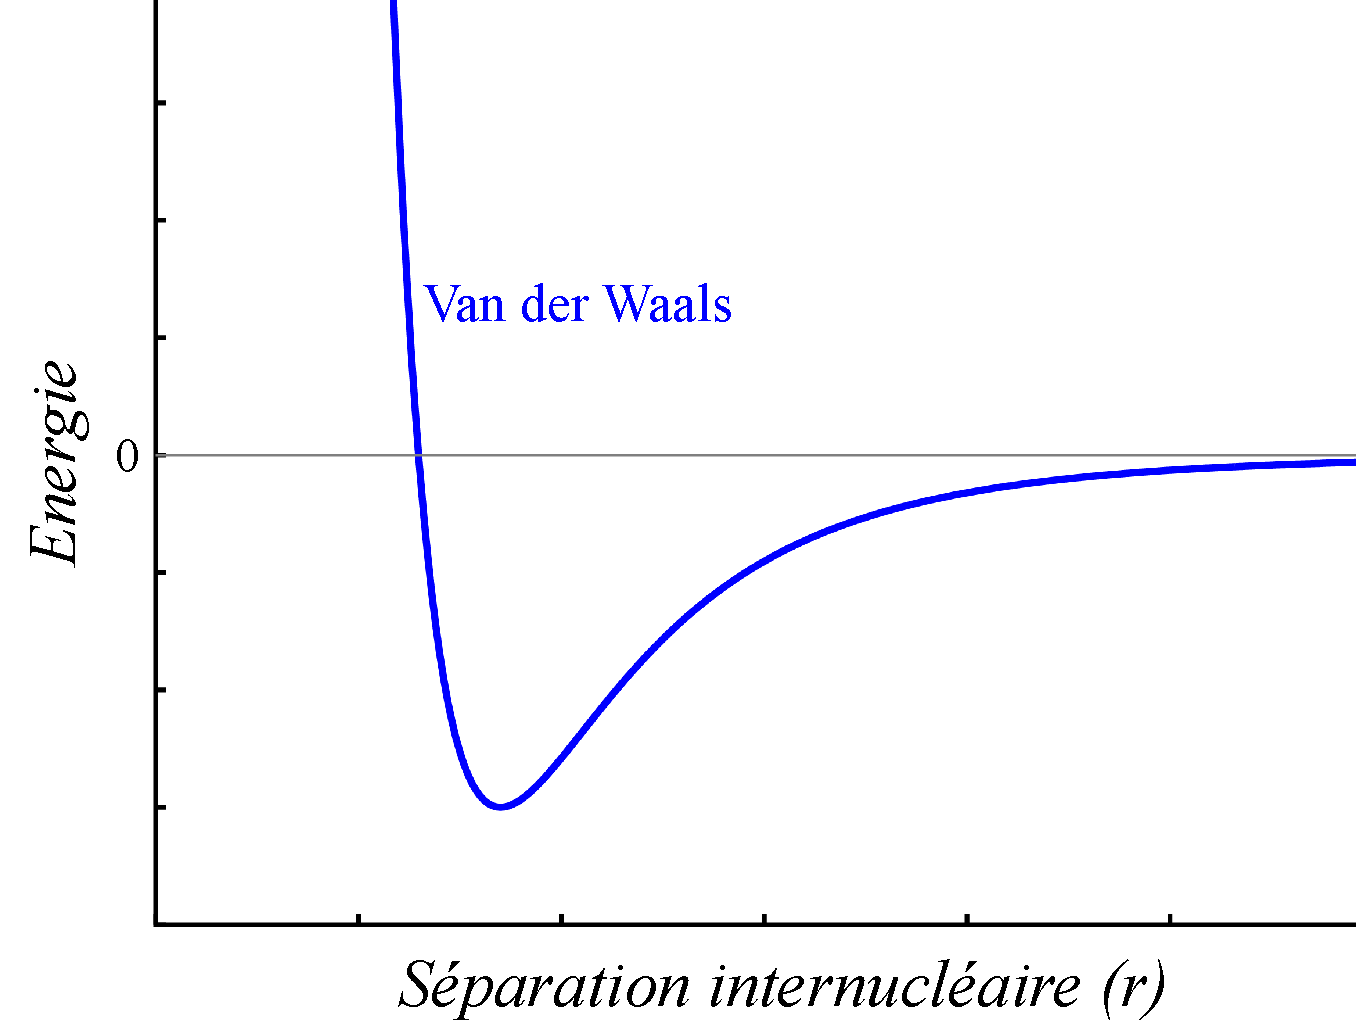
\includegraphics[height=5.3cm]{./figures/ch1/lennardjones.pdf}}
    \caption{}
    % \commentaire{MB: ce sont de vraies courbes, et a l'echelle? Car dans mon souvenir l'electrostatique devrait etre comparativement plus important (plus negative) vers la droite du graphe.}
    \label{Fig:lennardjones}
    \end{subfigure}
  \begin{subfigure}{.5\textwidth}
  \centering
  {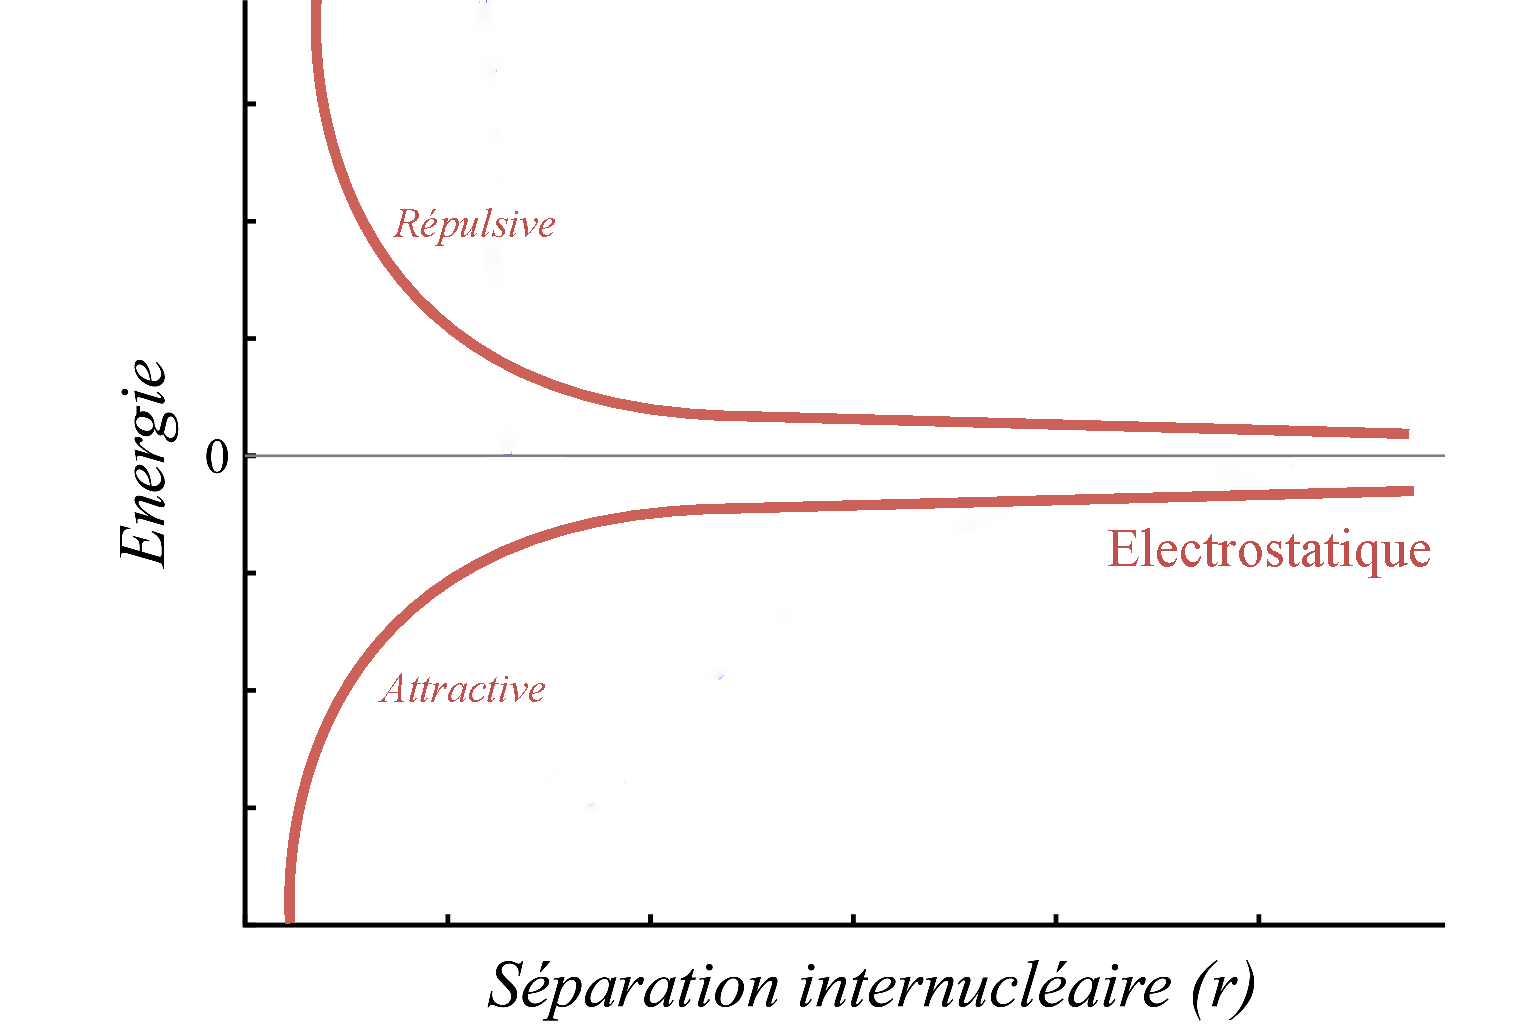
\includegraphics[height=5.3cm]{./figures/ch1/electrostatic.pdf}}
    \caption{}
    \label{Fig:electrostatic}
  \end{subfigure}
  \caption[Contributions énergétiques des forces électrostatiques et de van der Waals]{\it (a) Contributions énergétiques des forces de Van der Waals représentées par un potentiel de Lennard-Jones. La courbe garde la même forme quels que soient les atomes considérés.
  (b) Contributions énergétiques des forces électrostatiques représentées par un potentiel de Coulomb en fonction de la distance entre deux atomes. Des forces attractives prennent place entre deux atomes de charge différente alors que des forces répulsives prennent place entre deux atomes de même charge.}
  % \hspace{0.2cm}
\end{figure}


Les paramètres utilisés au sein des champs de force sont dérivés de données expérimentales, mais peuvent également être le résultat de calculs computationnels de mécanique quantique. Parmi les champs de force, certains décrivent la protéine de façon atomique en considérant chaque atome comme une particule et en appliquant des paramètres propres à chaque atome dans les équations. Ces champs de force, appelés \textbf{tout-atome}, malgré leur précision, souffrent d'un temps de calcul de leurs équations très important qui est un frein significatif pour l'évaluation énergétique de systèmes moléculaires de plus de quelques centaines/milliers d'atomes. Afin de permettre l'étude de protéines dépassant cette taille, il est possible de simplifier le champ de force. Dans ces champs de force simplifiés, appelés \textbf{gros grain}, le modèle de la protéine est différent puisque certains groupes d'atomes, groupes dont les propriétés physiques sont bien connues, sont considérés comme des particules uniques, réduisant ainsi le nombre de particules du système. La différence entre deux modèles de champs de force tout-atome et gros grain est illustrée dans la Figure \ref{Fig:coarse_grain_ff}. Une particule étant régie par un ensemble d'équations, réduire le nombre de particules revient à réduire le nombre de calculs à effectuer. Les chaînes latérales des acides aminés ainsi que les groupements méthyles sont deux exemples de groupements d'atomes dont la contribution énergétique est suffisamment approximée pour pouvoir être simplifiés. Dans le même but de simplification des calculs, certains atomes dont la contribution est considérée comme négligeable sont enlevés des champs de force, c'est souvent le cas des atomes d'hydrogène par exemple.

Le choix d'un champ de force dépend à la fois de l'environnement dans lequel est modélisé le complexe moléculaire d'intérêt ainsi que du degré de précision utilisé pour décrire les particules du système (tout-atome, atomes unifiés, gros grains, etc.). Parmi les champs de force les plus utilisés, nous pouvons citer CHARMM \cite{brooks2009charmm}, AMBER \cite{pearlman1995amber}, GROMOS \cite{oostenbrink2004biomolecular} ou OPLS \cite{jorgensen1996development}.

\begin{figure}[htb]
  \centering
  {\includegraphics[width=0.75\linewidth]{./figures/ch1/coarse_grain_ff.pdf}}
    \caption[Modèles de représentation d'un système moléculaire tout-atome et gros grain.]{\it Modèles de représentation d'un système moléculaire. A gauche, chaque atome est considéré indépendamment par une particule unique. A droite, chaque particule représente un ensemble d'atomes constituant un groupe particulier du système (molécules d'eau, chaînes latérales, chaînes principales, etc.\footnote{\url{http://www.ks.uiuc.edu/Research/cgfolding/}})}
    \label{Fig:coarse_grain_ff}
  \hspace{0.2cm}
\end{figure}

% \myparagraph{Paysage énergétique}

Les différentes valeurs d'énergie potentielle d'une protéine sont obtenues par la résolution de l'ensemble des équations des champs de force. Ces équations dépendent directement de la configuration spatiale de la protéine et constituent le paysage énergétique de cette protéine. Suivant l’objectif de la simulation, on cherchera soit à identifier le minimum global de ce paysage, soit à trouver des minima locaux traduisant des états structurels différents mais stables d'une protéine (voir Figure \ref{Fig:energy_landscape_edit}).


\begin{figure}
  \centering
  {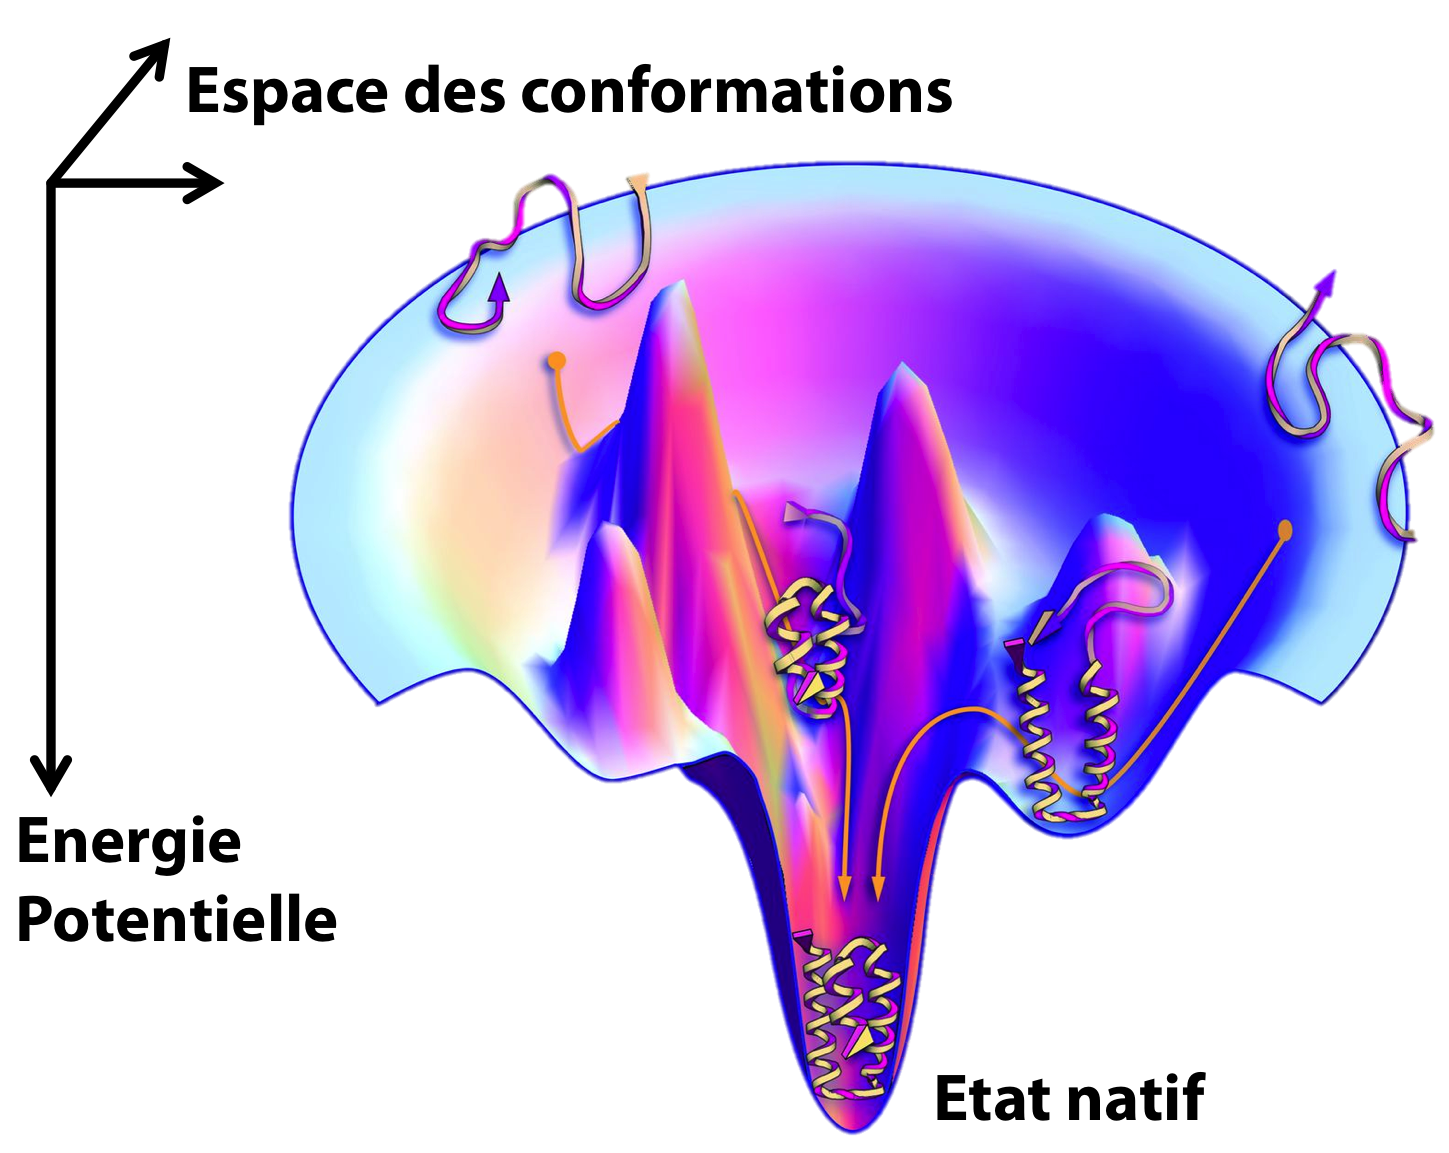
\includegraphics[width=0.65\linewidth]{./figures/ch1/energy_landscape_edit.png}}
    \caption[Représentation du paysage énergétique d'une protéine suivant sa conformation spatiale.]{\it Représentation d'un paysage énergétique d'une protéine suivant sa conformation spatiale. Plus l'énergie potentielle est haute, plus la protéine est considérée comme désordonnée et donc instable. Plusieurs puits d'énergie traduisant des minimas locaux peuvent être identifiés mais un seul minimum global existe correspondant à l'énergie de la conformation la plus stable de la protéine appelé également l'état natif de la protéine. Source : \cite{dill2012protein}}
    \label{Fig:energy_landscape_edit}
  \hspace{0.2cm}
\end{figure}
 

\subsubsection{Simulation moléculaire} \label{simu}


La simulation moléculaire cherche à modéliser l'état ou l'évolution d'un système de particules biologiques. Elle peut tenter de décrire un changement conformationnel ou le déroulement d'un phénomène impliquant plusieurs molécules.
Une protéine est rarement simulée dans le vide et il est commun d'ajouter au moins un modèle de solvant afin de se rapprocher au maximum des conditions réelles.

Plusieurs approches répondent aux différents besoins et applications de la simulation moléculaire. 
Les méthodes de mécaniques moléculaires simples ne prennent pas en compte l'énergie cinétique de l'environnement et sont plus rapides et adaptées à la recherche d'un état d'équilibre. Au contraire, la dynamique moléculaire ou les méthodes basées sur Monte-Carlo voient la simulation des conditions de température, pression, etc. influençant le comportement des particules pour calculer l'énergie du système, mais là où la notion de temps est présente en dynamique moléculaire, elle est absente de l'approche basée sur Monte-Carlo. La dynamique sera donc très adaptée pour l'étude de phénomènes moléculaires au cours du temps alors que les méthodes de Monte-Carlo seront davantage utilisées pour échantillonner les configurations possibles d'une protéine et parcourir son paysage énergétique.


\myparagraph{Mécanique moléculaire}

La mécanique moléculaire fait abstraction des paramètres thermodynamiques régissant les évolutions conformationnelles d'une structure protéique pour décrire de façon plus simple un système de particules en condition statique par la seule mécanique newtonienne. Elle repose sur l'utilisation de champs de force afin de calculer l'énergie potentielle d'une protéine. Ces différentes propriétés sont appliquées pour les modèles tout-atome :

\begin{itemize}
  \item Chaque atome est représenté par une particule unique
  \item Chaque particule possède un rayon, une polarisation et une charge nette constante
  \item Les interactions liées sont considérées comme des ressorts 
\end{itemize}

De façon plus précise, le rayon des particules est bien souvent le rayon de \textit{van der Waals} qui est une sphère géométrique théorique censée représenter l'espace occupé par un atome. La charge nette est dérivée de calculs expérimentaux ou quantiques afin d'être la plus proche possible de la réalité. Enfin, la distance à l'équilibre des ressorts représentant les liaisons est égale à la longueur expérimentale de la liaison.

L'application la plus directe et courante de la mécanique moléculaire est la minimisation énergétique où l'on va chercher à obtenir des modèles avec une énergie de plus en plus faible afin de trouver la structure 3d la plus stable pour une protéine donnée. Les algorithmes de minimisation moléculaires sont divers, mais ils se basent très souvent sur les champs de force de mécanique moléculaire.

\myparagraph{Dynamique moléculaire}

Le principe de la dynamique moléculaire (MD) repose sur la résolution d'équations thermodynamiques respectant les lois énoncées en mécanique moléculaire afin de guider les particules décrivant la protéine vers des configurations spatiales différentes. Son but est donc de simuler les mouvements de particules dans le temps pour des conditions thermodynamiques (température, pression, etc.) précises tout en prenant en compte la mécanique newtonienne régissant les contributions énergétiques de ces particules.

Au sein des publications scientifiques de ces dernières années, les échelles de temps des processus biologiques simulés vont de quelques nanosecondes ($10^{-9}$s) à quelques microsecondes ($10^{-6}$s). Ces échelles de temps biologiques correspondent de plusieurs jours à plusieurs années de calculs computationnels. Cependant, la parallélisation au sein de CPU et maintenant de GPU permet de diviser ces temps par un facteur allant de 10 à quelques milliers afin d'obtenir des temps de calcul s'étalant sur quelques semaines au maximum.

Une dynamique moléculaire introduit, à la différence des deux méthodes précédentes, la notion de mouvement atomique qui se caractérise par la formule donnée par la 2nde loi de Newton :

$$F_i = m_i.a_i$$

où $F_i$ représente la somme des forces exercées sur l'atome $i$ de masse $m_i$ et d'accélération $a_i$. On obtient la force localisée sur un atome en dérivant l'énergie du système entier par rapport à la position de l'atome. A chaque pas de temps on obtiendra ainsi une nouvelle position de l'ensemble des atomes et il est possible d'évaluer l'énergie potentielle du système grâce au champ de force utilisé.

% Le modèle 3d de la protéine au départ de la simulation est souvent intégré dans un environnement atomique, modélisé informatiquement, cherchant à refléter le plus fidèlement possible l'environnement cellulaire dans lequel la protéine évolue \textit{in vivo}. Cet environnement peut être représenté simplement au moyen d'une boîte virtuelle contenant des molécules d'eau où la protéine sera plongée, ceci constitue un des environnements les plus basiques et les plus utilisés. Dans des environnements plus complexes, il est possible de retrouver les ions présents habituellement autour de la protéine ou des structures complexes représentant une partie de composant cellulaire au sein duquel évolue habituellement le complexe moléculaire étudié telle que la membrane cellulaire. Il est possible d'utiliser un solvant explicite ou implicite pour représenter l'environnement. Les solvants explicites regroupent des particules dont la trajectoire et le comportement devront être calculés explicitement par le champ de force. Ces particules se conformeront aux mêmes types de paramètres physico-chimiques définissant les atomes de la protéine. 
% La boîte de simulation contenant l'ensemble des particules de la protéine et de l'environnement est de taille limitée afin de réduire le volume de simulation et restreindre le nombre calcul. Cependant, les différents bords de la boîte agissent de manière périodique de façon à ce qu'aucune contrainte physique ne s'applique en cas de choc avec les atomes du système. La périodicité assure aussi une homogénéité du nombre de particules puisque les atomes franchissant une limite de la boîte sont transportés sur la face opposée tout en gardant leurs propriétés de vitesse et d'accélération.

% Dans le cas de solvant implicite, un potentiel de force moyen est introduit dans le champ de force afin de rendre compte des interactions protéine/solvant. Ainsi une énergie de solvatation est calculée et intégrée dans le calcul d'énergie potentielle. Deux types de méthodes permettent de rendre compte de la contribution de cette énergie de solvatation: la résolution de l'équation de \textit{Poisson-Boltzmann} et le modèle de \textit{Born} généralisé.

% Lorsque la structure de départ et l'environnement ont été définis, la simulation moléculaire peut débuter. Une simulation moléculaire se caractérise par l'obtention des accélérations, des vitesses et finalement des positions depuis les forces et les potentiels d'interaction des particules. Les trajectoires des particules peuvent être calculées par différents algorithmes, les plus utilisés et connus étant:

% \begin{itemize}
%   \item La méthode d'\textbf{Euler} est la procédure la plus élémentaire qui permet de déterminer de façon numérique la trajectoire d'une particule soumise à une somme de forces $\overrightarrow{F}$ connue. Elle se base sur la 2e loi de Newton qui énonce:
%   $$\overrightarrow{a} = \frac{\overrightarrow{F}}{m}$$
%   Elle se base sur le calcul de la vitesse et de la position à chaque pas de temps suivant ces deux équations:

%   $$\overrightarrow{x}(n+1) = \overrightarrow{x}(n) + \overrightarrow{v}(n)\Delta t$$
%   $$\overrightarrow{v}(n+1) = \overrightarrow{v}(n) + \overrightarrow{a}(n)\Delta t$$

%   où $\overrightarrow{x}$ désigne la position, $\overrightarrow{v}$ désigne la vitesse et $\overrightarrow{a}$ l'accélération d'une particule.
%   Les valeurs pour un pas de temps précis dépendent donc uniquement du pas de temps précédent. Les hypothèses permettant d'utiliser la méthode d'Euler sont: (1) on connaît les valeurs pour le pas de temps initial, (2) ce pas de temps est fixe tout au long de la simulation. La simplicité de la méthode est contrebalancée par son manque de précision et de stabilité.
%   \item L'intégration \textbf{leapfrog} est une version modifiée de l'algorithme d'Euler sur laquelle elle repose. Elle se base sur un calcul de la vitesse et des positions décorrélées puisque la vitesse va être calculée pour des pas de temps "demi-entiers". Ce qui se traduit par les deux équations suivantes pour les calculs:

%   $$\overrightarrow{x}(t+1) = \overrightarrow{x}(t) + \overrightarrow{v}(t+\frac{1}{2})\Delta t$$
%   $$\overrightarrow{v}(t+\frac{1}{2}) = \overrightarrow{v}(t-\frac{1}{2}) + \overrightarrow{a}(t)\Delta t$$

%   Les équations ressemblent beaucoup à celles d'Euler, mais la différence vient de l'initialisation. Le couple ($\overrightarrow{x}(0),\overrightarrow{v}(0)$) est bien donné, mais, pour la vitesse, est donné également:

%   $$\overrightarrow{v}(\frac{1}{2}) = \overrightarrow{v}(0) + \overrightarrow{a}(0)\frac{\Delta t}{2}$$

%   De cette façon, la position et la vitesse vont jouer à saute-mouton à tour de rôle l'un par-dessus l'autre. Cette version "saute-mouton" de la méthode d'Euler a une meilleure conservation de l'énergie est invariante par renversement.
%   \item L'intégration de \textbf{Verlet pour les positions}. Cet algorithme cherche à calculer les positions du prochain pas de temps grâce aux positions du pas de temps courant et du pas de temps omettant donc le facteur vitesse. L'équation appliquée pour obtenir une position est la suivante: 

%   $$\overrightarrow{x}(t +\Delta t) = 2\overrightarrow{x}(t) - \overrightarrow{x}(t - \Delta t) + \overrightarrow{a}(t)\Delta t^2 + O(\Delta t^4)$$ 

%   où $\overrightarrow{x}$ désigne une position et $\overrightarrow{a}$ l'accélération.
%   On remarque qu'un éventuel problème pourrait survenir pour la première position calculée puisqu'aucune information sur un pas de temps précédent n’existe. Cependant, l'accélération à t$_0$ est connue et permet, grâce au théorème de Taylor, d'approximer la position initiale avec une erreur d'ordre de grandeur négligeable ($O(\Delta t^3)$) en comparaison de l'erreur totale cumulée au cours de la simulation d'ordre de grandeur $O(e^{Lt_n}\Delta t^2)$.
%   \item L'intégration de \textbf{Verlet pour les vitesses} se rapproche de la méthode <<leapfrog>> à l'exception du fait qu'elle calcule la position et la vitesse aux mêmes valeurs de pas de temps. L'approche est identique, mais incorpore explicitement la vitesse, résolvant ainsi le problème du premier pas de temps de l'intégration de Verlet pour les positions. L'algorithme peut être simplifié et résumé dans ces 3 étapes:
%   \begin{enumerate}
%     \item On calcule: $\overrightarrow{x}(t+\Delta t) = \overrightarrow{x}(t) + \overrightarrow{v}(t)\Delta t + \frac{1}{2}\overrightarrow{a}(t)\Delta t^2$
%     \item On dérive $\overrightarrow{a}(t+\Delta t)$ à partir du potentiel d'interaction en utilisant $\overrightarrow{x}(t+\Delta t)$
%     \item On calcule: $\overrightarrow{v}(t+\Delta t) = \overrightarrow{v}(t) + \frac{1}{2} (\overrightarrow{a}(t) + \overrightarrow{a}(t+\Delta t))\Delta t$
%   \end{enumerate}
%   Cet algorithme suppose que l'accélération $\overrightarrow{a}(t+\Delta t)$ dépend seulement de la position $\overrightarrow{x}(t+\Delta t)$ et ne dépend pas de la vitesse $\overrightarrow{v}(t+\Delta t)$.
%   \item La méthode \textbf{Runge-Kutta} (ou prédicteur-correcteur) possède plusieurs ordres d'application. La méthode RK1 (d'ordre 1) est une simple application de la méthode d'Euler. La méthode RK2 du point milieu est unec composition de la méthode d'Euler qui consiste à estimer la dérivée au pas de temps $t$ pour obtenir la position au demi-pas de temps suivant $t+\frac{\Delta t}{2}$ puis de recalculer la dérivée de ce nouveau point pour estimer le point au pas de temps $t+\Delta t$. La méthode RK4 se base sur le même principe, calculant ainsi la position $\overrightarrow{x}(t+\Delta t)$ grâce à la position $,,\overrightarrow{x}(t)$ mais également en fonction du comportement approché en 3 points intermédiaires. Le comportement de ces points intermédiaires est approché en utilisant à chaque fois la dernière pente connue. Ainsi, chaque nouvelle position tous les pas de temps nécessite 4 évaluations à la différence des 2 évaluations de la méthode d'Euler par exemple.
% \end{itemize}


% Le choix de l'algorithme à appliquer est difficile du fait de la précision relativement importante qu'elles fournissent toutes. La méthode d'Euler, d'ordre 1, possède deux avantages notables sur les méthodes d'ordre supérieur que soient les intégrations \textbf{leapfrog} ou \textbf{Runge-Kutta}: (1) dans le cadre des simulations moléculaires, les forces mises en jeu sont telles qu'il est nécessaire de prendre un pas de temps réduit pour rendre compte d'une précision acceptable de la trajectoire. Or, à des pas de temps très proches, les méthodes d'ordre 1 possèdent une précision presque aussi importante que les méthodes d'ordre supérieur. (2) Les ressources calculatoires nécessaires pour l'application des méthodes d'ordre supérieur à 1 sont significativement plus importantes que celles nécessaires aux méthodes d'ordre 1. Pour des trajectoires se déroulant sur une période de temps un peu longue, le gain en précision ne justifie pas le temps de calcul dédié à la simulation.  

Le facteur de temps dans les simulations de MD évolue dans un espace discret et tout au long de la simulation, les coordonnées 3d de la structure sont sauvegardées à des pas de temps réguliers afin de pouvoir rejouer la trajectoire de la simulation à tout moment au moyen de programmes de visualisation 3d. Chaque pas de la simulation correspond à un ensemble de coordonnées 3d qui est associé à une valeur d'énergie potentielle.

Les programmes de dynamique moléculaire les plus connus regroupent plusieurs programmes basés exclusivement sur les champs de force qu'ils utilisent : AMBER, GROMACS ou CHARMM tiennent leur nom de leur champ de force (AMBER, GROMOS et CHARMM respectivement) et sont les plus utilisés dans la communauté de modélisation moléculaire. Nous pouvons aussi citer NAMD\footnote{\url{http://www.ks.uiuc.edu/Research/namd/}} \cite{phillips2005scalable} spécialisé dans la dynamique moléculaire parallélisée souvent utilisé pour simuler de grands systèmes moléculaires de plusieurs millions d'atomes.

\myparagraph{Minimisation moléculaire}

Il s'agit de trouver le minimum de la fonction qui permet de retrouver l'énergie potentielle de la molécule en fonction de sa géométrie. Il s'agit plus précisément de trouver des puits d'énergies le long du paysage énergétique de la protéine reflétant les conformations structurelles les plus stables de la protéine (voir Figure \ref{Fig:energy_landscape_edit}). Cette minimisation peut emprunter plusieurs algorithmes pour parvenir à ses fins mais le principe central reste le même. Il s'agit de bouger les atomes d'un système afin de minimiser l'énergie à chaque déplacement d'atomes. Chaque pas de la minimisation va évaluer l'impact énergétique du déplacement et ainsi décider si celui-ci est stabilisant pour la structure ou perturbant. Cette évaluation est faite via la résolution des fonctions du champ de force et du calcul de l'énergie potentielle.


\myparagraph{Algorithme de Monte-Carlo}

La méthode de simulation basée sur Monte-Carlo est l'une des plus usitées \cite{metropolis1949monte} consiste en un échantillonnage aléatoire des différentes configurations spatiales d'un système moléculaire. Les changements entre les configurations sont des changements induits de façon statistique et se caractérisent par la perturbation de la longueur d'une liaison, d'un angle, d'un angle dièdre ou le léger déplacement d'un atome ou d'un groupe d'atomes. 
Il est possible de décrire le principe général d'une simulation utilisant la méthode de Monte-Carlo de la manière suivante :

\begin{enumerate}
  \item Calcul de l'énergie du système dans son état $n$ grâce aux équations du champ de force utilisé => U($n$)
  \item Changement aléatoire pour obtenir une nouvelle conformation spatiale $n$+1
  \item Calcul de l'énergie du système dans son état $n$+1 => U($n$+1)
  \item Test d'acceptabilité: 
  Si U($n$+1) est inférieur à U($n$) alors le changement est accepté et la conformation $n$+1 est gardée. 
  Si U($n$+1) est supérieur à U($n$) alors on évalue le changement selon l'équation : $acc(n -> n+1) = min(1, exp(-(U(n+1)-U(n))/kT))$ où k est la constante de Boltzmann et T la température du système. Dans cette équation, le facteur de Boltzmann ($exp(-(U(n+1)-U(n))/kT)$) est comparé avec un nombre aléatoire compris entre 0 et 1. Si le nombre aléatoire est plus grand que le facteur de Boltzmann alors la conformation est rejetée, sinon, elle est acceptée.
  \item Le processus reprend à l'étape 1 avec l'état $n$ ou $n$+1 suivant le résultat de l'étape précédente.
\end{enumerate}



% Des informations expérimentales complémentaires peuvent servir de guides pendant la simulation et vont venir orienter les changements structurels d'un complexe vers un état structural approximé et connu. Il est ainsi possible de réduire le chemin énergétique qu'il aurait fallu pour atteindre un état stable préalablement identifié.

% \myparagraph {Simulation moléculaire interactive} \label{simu_interactive}

% Certaines simulations moléculaires, couplées à de rendus graphiques très performants et des dispositifs d'interactions adaptés, permettent à l'utilisateur de contraindre certaines parties d'une structure moléculaire pendant sa simulation en injectant dans les calculs physiques des forces s'appliquant sur les particules manipulées \cite{bolopion_comparing_2010}. Le jeu sérieux Foldit\footnote{\url{https://fold.it/portal/}} s'appuie sur les stratégies et l'esprit d'analyse des utilisateurs, experts ou non du domaine, pour guider les changements conformationnels de protéines par des commandes simples. Un score est calculé en temps réel permettant de rendre compte de la stabilité énergétique de la structure obtenue. Alors que le chemin énergétique suivi par un algorithme standard va favoriser les changements conformationnels peu coûteux, l'esprit humain est capable d'anticiper un changement qui va contraindre la protéine de façon importante, mais permettant d'obtenir une structure plus stable par la suite \cite{khatib2011crystal}.

% Il est également possible de générer des représentations volumiques de certaines informations expérimentales comme des cartes de densité de données cristallographiques ou SAXS afin de permettre à l'utilisateur d'agir sur les domaines flexibles de sa protéine afin de la faire entrer dans ces volumes. Certains projets utilisent même directement l'aide de l'utilisateur afin de replier une protéine représentée grâce à des paramètres de mécanique moléculaire et déplacée/orientée dans une carte de densité électronique SAXS \cite{molza2014innovative,tek2012advances}.

% La possibilité d'influer ainsi sur une simulation moléculaire demande la mise en place d'une structure logicielle de haute performance, car des modules s'occupant de la simulation en elle-même, de la visualisation de l'évolution de la simulation et de la gestion des interactions homme-machine doivent fonctionner de façon synchronisée.
% La représentation simplifiée de la protéine permet une certaine rapidité de la simulation et donc la prise en compte rapide de l'effet des changements opérés par l'utilisateur. Dans cette optique, le projet BioSpring permet la représentation de protéines par des réseaux de ressorts pour les interactions liées et des paramètres de champ de force configurables pour les interactions non liées \cite{ferey2012biospring}. Cette représentation semi-simplifiée permet de contraindre les parties rigides de la protéine tout en assurant une certaine flexibilité au niveau des régions moins structurées (boucles et coudes).

% Dans le cas de dynamiques moléculaires sur des systèmes de taille plus importante, calculées dans des clusters de calcul déportés, les défis sont autres. Ils passent par la mise en place de communications privilégiées entre le centre de calcul et le lieu de visualisation et d'interaction (il est rare de retrouver des espaces de visualisation dédiés au sein même des centres de calcul). En plus des communications, la précision demandée peut être supérieure et les forces appliquées au système doivent pouvoir être interprétées de façon instantanée par le programme de simulation. Des suites logicielles performantes permettent aujourd'hui de traiter une simulation de façon interactive alors même que cette dernière est déportée \cite{dreher2014exaviz}. Basée sur les principes de parallélisation d'instructions et d'utilisation des infrastructures de communications récentes offrant des vitesses de transmission de données au-delà de 10Gbit/s.

% Il se calcule de la manière suivante:

% $$GDT\_TS = 100\frac{\sum_dGDT_d/N}{4}\%\ d\in\{1,2,4,8\}$$

% où $N$ est le nombre total de résidus d'un modèle, $GDT_d$ est le nombre de résidus alignés dont la distance des carbones alpha entre le modèle prédit et la structure native est moins de $d$\r{A} après superposition des deux structures (prédite et native); et $d$ est 1,2,4 ou 8\r{A}.
% Ce score basé uniquement sur la distance peut être associé à d'autres scores basés sur les connaissances comme des scores d'alignement qui vont ainsi traduire de la pertinence biologique du modèle prédit basé sur son éloignement des standards présents dans les bases de données.

\subsubsection{Folding moléculaire ou prédiction de structure tertiaire} 

La prédiction de structure tertiaire d'une protéine consiste à retrouver la structure 3d naturelle d'une protéine à partir de sa séquence primaire. Cette prédiction de structure est également appelée \textit{folding} moléculaire (ou repliement en français) car elle peut permet d'obtenir des informations sur le processus de repliement des protéines 

Lorsque aucune information ne peut être utilisée pour cette prédiction, on parle de prédiction \textit{ab initio}, prédiction passant souvent par la prédiction préalable de la structure secondaire de la protéine. Cette première étape de prédiction peut passer par : (1) des méthodes statistiques attribuant une probabilité de structuration en feuillet/hélice/coude par acide aminé, (2) des approches physico-chimiques en cherchant à calculer les interactions interatomiques et donc appliquant les forces d'attraction/répulsion pour obtenir une structure ou (3) un alignement et comparaison évolutive en protéines de la même famille dont la structure secondaire est connue.
Lorsque la structure secondaire est connue, il est possible d'effectuer une simulation moléculaire afin d'utiliser des paramètres physico-chimiques pour diriger le repliement des motifs de structures secondaires identifiés. Les changements conformationnels menant de la structure de départ au modèle 3d final sont souvent importants puisque aucune information préalable n'est utilisée.

Il est évidemment possible de s'appuyer sur des informations expérimentales existantes afin de prédire la structure 3d d'une protéine. Parmi les informations utilisées, les bibliothèques de fragments ou alphabets structuraux permettent d'obtenir la structuration la plus retrouvée pour différentes séquences d'une dizaine d'acides aminés. 
Il est également possible de s'intéresser aux protéines dont la structure 3d est déjà connue. Grâce à un alignement global de la séquence de la protéine étudiée il est possible d'identifier des protéines possédant une similarité de séquence significative (> à 30\%) et ainsi structurer la protéine à prédire à partir des motifs structuraux connus; il s'agit de la modélisation par homologie.
Une dernière méthode de prédiction est la méthode de \textit{threading} qui voit l'enfilage de courtes séquences d'acides aminés au sein de structures 3d répertoriées comme courantes au sein de banques de données de structures 3d de protéines. Chaque enfilage donne lieu à un calcul d'énergie des acides aminés ainsi contraints dans un carcan 3d et les structures 3d de plus basses énergies sont considérées comme les candidats les plus probables pour structurer la protéine.

% La prédiction de structure 3d est un domaine plus vaste et plus complexe puisqu'elle cherche à obtenir la configuration spatiale d'une protéine à l'état stable et donc fonctionnel. Il est possible de détacher trois types d'approches pour la prédiction de structure tertiaire:

% \myparagraph{Approches \textit{ab initio}} \label{ab_initio}

% Elles ont pour but de prédire la structure tridimensionnelle à partir de la seule séquence primaire, sans autres informations structurelles provenant de structures de protéines proches déjà résolues. Le processus de prédiction se base très souvent sur des structures secondaires prédites (voir \ref{prediction_struct_second}) et non pas sur une structure 3d complètement aléatoire construite à partir de la seule séquence en acide aminé. 
% Les méthodes qui sont mises en jeu en prédiction \textit{ab initio} se basent sur les seuls principes physiques régissant le repliement des protéines. Ce repliement intervient après l'étape de traduction et avant l'éventuel déplacement de la protéine vers son lieu d'action. Nous avons vu qu'il mettait en jeu certaines molécules <<chaperonnes>> afin d'aider la molécule à atteindre sa forme stable. Il est cependant très difficile d'intégrer les mécanismes impliquant ces molécules et la grande majorité des modélisations \textit{ab initio} ne s'appuie que sur les énergies mises en jeu dans la protéine même pour induire le repliement. En moyenne, l'étape de repliement se déroule en quelques millisecondes même si certaines molécules se replient en quelques microsecondes. Ces temps de repliement, bien que très court à l'échelle humaine, sont des temps extrêmement longs à simuler informatiquement.

% Même si le problème de la prédiction \textit{ab initio} systématique à partir de la séquence primaire est encore largement irrésolu, il est désormais possible de prédire la structure 3d de petites protéines à domaine unique à environ 1.5 \r{A} de précision pour l'ensemble de la structure. Pour les protéines de plus grandes tailles, le problème est complexe, car il nécessite des capacités de calcul très important.

% L'étape centrale de la prédiction \textit{ab initio} est l'application des méthodes de résolution stochastiques pour l'optimisation globale de fonction d'énergies. Afin de ne pas exploser le temps de calcul nécessaire à la génération d'un modèle pour une protéine de taille standard, ce seront des champs de force gros grains qui seront préférés pour la modélisation de son repliement.

% En plus de la simplification des modèles de particules utilisés au sein des champs de force, il est aussi possible de cibler le coeur du problème en prédiction \textit{ab initio} qui est la puissance de calcul brute. Des méthodes de distribution des capacités de calcul (ou crowdcomputing) ont été mises en place à travers des projets comme \textit{Folding@home}\footnote{\url{https://folding.stanford.edu/}} ou \textit{Rosetta@home}\footnote{\url{https://boinc.bakerlab.org/}} qui s'appuient sur les capacités de calculs d'ordinateurs particuliers ou de clusters d'instituts scientifiques ou non pour faire fonctionner des algorithmes parallélisés de repliement protéique. L'idée est donc de répartir les ressources nécessaires pour les calculs de simulation sur un maximum de machines dans le monde.

% \myparagraph{Approches \textit{de novo}}

% Ces approches sont très proches de celles dites \textit{ab initio} dans leur principe. La principale différence se situe au niveau des données utilisées en entrée. À la différence des méthodes précédentes, les méthodes \textit{de novo} incluent des données expérimentales afin de guider la prédiction. Parmi les données expérimentales utilisées, les bibliothèques de fragments ou d'alphabets structuraux fournissent des sous-ensembles d'acides aminés (séquence de 4 à 15 acides aminés environ) dont les angles dièdres sont définis et dont la configuration spatiale est retrouvée dans certaines protéines de la PDB pour (\textit{Protein Data Bank}, base de données spécialisée de structures moléculaires décrite dans la section \ref{protein_DB}). L'algorithme le plus connu et utilisé est certainement Rosetta, développé par David Baker et son équipe \cite{rohl2004protein}. Il se base sur l'hypothèse que les structurations locales de la protéine ont un impact, mais ne définissent pas totalement la configuration spatiale globale de la protéine. L'algorithme se base sur l'assemblage de fragments structuraux de plusieurs acides aminés (9 acides aminés en phase 1, 3 acides aminés en phase 2) respectant la séquence primaire de la protéine prédite. Ces fragments ont une structure connue et sont récupérés depuis des bibliothèques de fragments basés sur la PDB. Les fragments sont positionnés de façon aléatoire et sont évalués par une simulation Monte-Carlo afin de leur attribuer un score. Chaque nouvel assemblage de fragments positionnés aléatoirement va donc générer un modèle avec un score associé. Les modèles avec les meilleurs scores seront considérés comme les plus stables énergétiquement et donc les plus proches de la structure tertiaire recherchée.

% \myparagraph{Approches par homologie} 
% Elles utilisent la connaissance des structures de protéines proches de la protéine étudiée. Un alignement de séquence est effectué afin d'identifier, parmi les protéines dont la structure tridimensionnelle a été résolue, les séquences primaires homologues à la séquence de la protéine étudiée. On considère deux séquences comme homologues lorsque leur similarité est supérieure à 30\%. Les différentes étapes de la modélisation par homologie sont:
% \begin{enumerate}
% 	\item La sélection du modèle se fait grâce à un alignement multiple de la séquence cible grâce à des algorithmes spécialisés comme BLAST\footnote{\url{http://blast.ncbi.nlm.nih.gov/Blast.cgi}} ou PSI-BLAST appliqué sur l'ensemble des séquences de la PDB. Les séquences avec des similarités de séquences supérieures à 30\% sont des candidates pour être des modèles structuraux. Cependant, la similarité de séquence pure n'est pas le meilleur indicateur de l'homologie entre deux séquences protéiques. Au lieu de prendre en compte une similarité faible sur la séquence entière, on favorise la présence de plusieurs régions très similaires le long de la séquence. Ces régions de forte similarité dénotent souvent d'un caractère évolutif proche et de séquences conservées et donc potentiellement importantes pour la fonction de la protéine. On considère qu'il est possible d'obtenir des modèles par homologie de bonne qualité lorsque le degré de similarité entre la séquence cible et la séquence modèle est supérieur à 50\%.
% 	\item La chaîne principale des acides aminés composant la séquence modèle fournit la structure du <<noyau>> de la configuration spatiale prédite au niveau des régions très structurées (hélices et feuillets) et dont la séquence est souvent bien conservée entre séquences homologues. Les angles des liaisons du squelette sont reportés dans le modèle afin de reproduire les motifs de structure secondaire.
% 	\item Les régions non structurées de la structure 3d sont modélisées par des boucles. Ces boucles sont des régions non retrouvées dans la séquence modèle et dont les informations structurelles doivent être obtenues soit grâce à des bases de données spécialisées ou par l'utilisation de méthodes \textit{ab initio}.
% 	\item La prochaine étape de la conception du modèle est l'ajout des chaînes latérales suivant la séquence de la protéine cible afin de donner la configuration spatiale finale de la protéine. Ces chaînes latérales ont un degré de liberté variable selon leur nature ce qui rend leur assignation particulièrement difficile. Il existe cependant des librairies de rotamères (conformations rotationnelles autour d'une liaison simple) qui décrivent les angles adoptés par les éléments composants les chaînes latérales suivant la conformation de la chaîne principale. Le nombre de conformations est limité par les contraintes stéréochimiques (arrangement spatial des atomes) et énergétiques.
% 	\item Finalement, il est possible et très courant d'affiner le modèle par minimisation d'énergie ou dynamique moléculaire (voir section \ref{simu}) afin de supprimer l'encombrement stérique des chaînes latérales (gêne provoquée par la disposition et le volume des chaînes latérales entraînant une instabilité locale dans la protéine) et la mise en conformité des valeurs d'angles entre tous les atomes. Cela permet de minimiser l'énergie potentielle du système et donc d'obtenir un modèle pertinent d'un point de vue physico-chimique.
% \end{enumerate}

% Parmi les outils de modélisation par homologie, WhatIf\footnote{\url{http://swift.cmbi.ru.nl/whatif/}} et Modeller\footnote{\url{https://salilab.org/modeller/}} sont tous les deux très utilisés au sein de la communauté scientifique.

% \myparagraph{Approches par \textit{threading}}

% Les méthodes de \textit{threading} peuvent être décrites comme l'inverse des méthodes d'homologie. Le principe repose sur l'enfilage de séquences d'acides aminés sur des structures 3d déjà identifiées et présentes dans la PDB. Les acides aminés de la protéine prédite sont donc contraints structurellement afin de s'aligner sur la structure modèle et l'énergie du système est alors calculée. Cette fonction de score doit témoigner de la similarité séquence-structure et permettre le classement des structures utilisées afin d'identifier les modèles de moindre énergie.
% Cette approche se base sur deux observations: le nombre de conformations spatiales différentes dans la nature est relativement réduit (environ 1300) et 90\% des nouvelles structures ajoutées dans la PDB ces trois dernières années ont des conformations spatiales similaires à celles déjà présentes au sein de la base de données.
% La rapidité de cette méthode est un atout non négligeable pour la prédiction de structures tertiaires et son utilisation de bases de données structurelles telles que SCOP ou CATH en fait une méthode biologiquement pertinente.



\subsubsection{Docking moléculaire ou amarrage protéine-protéine}

Le docking moléculaire (ou \textit{amarrage} moléculaire en français) consiste à prédire l'orientation et la configuration spatiale d'une molécule par rapport à une seconde lorsqu’elles se lient pour former un complexe moléculaire stable. Ce domaine de la modélisation moléculaire est de grande importance, car la quasi-exclusivité des réactions métaboliques se déroulant au sein d'un organisme se traduit par la liaison de deux ou plusieurs molécules entre elles. C'est notamment le cas des protéines dont les fonctions sont dirigées par leur capacité à se lier à des partenaires moléculaires afin d'induire différents effets. Ces partenaires peuvent être de différentes natures : acides nucléiques (en particulier pendant les étapes de transcription et traduction), autres protéines, petites molécules (avec souvent un rôle activateur ou inhibiteur), etc.

Parmi les applications les plus importantes du docking moléculaire, la conception de médicaments dont les constituants vont se lier à une cible moléculaire pour un effet agoniste ou antagoniste est un domaine où les méthodes de docking jouent un rôle primordial.
% Dans le domaine du docking protéine-partenaire, il est commun de considérer une protéine réceptrice sur laquelle va se lier un ligand. Ce ligand, pouvant être de différentes natures, va être manipulé afin de se lier à la protéine, cette dernière étant considérée comme fixe. On parle de forme, de structure ou de protéine non liées lorsqu'on s'intéresse à la structure individuelle d'une protéine alors qu'on évoque une forme liée pour désigner la structure d'une protéine en complexe et donc liée à son partenaire moléculaire. 
% La protéine réceptrice possède dans la majorité des cas une conformation 3d non liée connue, ce qui n'est pas toujours le cas du ligand. Il existe des exceptions à ces règles que nous détaillerons par la suite. La connaissance du ligand est primordiale, car sa nature va souvent influencer son degré d'affinité avec la protéine et va mettre en jeu des mécanismes différents suivant sa taille, ses propriétés de surface ou sa flexibilité. Les protéines de petite taille (moins de 50 acides aminés) ont par exemple tendance à se lier de façon très transitoire avec la protéine réceptrice, entraînant ainsi des affinités de liaison très faibles et difficiles à évaluer, en plus de leur grande flexibilité. Les protéines venant se lier sur d'autres protéines vont elles se lier de façon plus longue et mettre en jeu des énergies plus importantes au niveau d'interfaces plus planaires que pour des petites molécules.

Une image souvent utilisée pour représenter le concept de docking moléculaire est le problème du verrou et de la clé. L'idée de ce problème est de trouver le trou, site de liaison de la clé, puis l'orientation correcte de la clé pour ouvrir le verrou. La protéine serait le verrou dont le trou se trouverait à sa surface et le ligand constituerait donc la clé.

% Cette métaphore nous montre bien les deux étapes indispensables au docking moléculaire et qui composent la majorité des programmes de docking existants. Une première étape est la recherche du site de liaison du ligand à la surface de la protéine. Lorsque des sites candidats sont trouvés, alors différentes configurations spatiales ou orientations du ligand sont testées au contact de ces sites, ceci constitue la seconde étape. Ces deux étapes sont indépendamment longues et coûteuses et il n'est pas rare de voir chacune de ces étapes être dirigée par deux programmes différents.

Lorsqu'on s'intéresse au docking \textit{ab initio}, où aucune information n'est utilisée sur le potentiel site de liaison, deux approches peuvent être identifiées afin de générer un modèle 3d de complexe fonctionnel entre la protéine et son ligand.

La \textbf{complémentarité de forme} considère la protéine et le ligand du point de vue des propriétés géométriques et physiques de leur surface. Parmi les descripteurs utilisés pour représenter la protéine et son ligand, la surface accessible au solvant (SAS) pour la protéine et des descriptifs de complémentarité de surface pour le ligand peuvent être utilisés \cite{shoichet1992molecular}. Un autre descripteur décrit les paramètres hydrophobes de la protéine. Des patchs hydrophobes et leurs opposés hydrophiles peuvent ainsi aider à identifier les sites de liaison et mettre de côté les régions peu propices à être en contact avec une autre protéine \cite{jones1996principles}. Une fois que les paramètres géométriques sont analysés et utilisés pour rapprocher les deux partenaires, une minimisation moléculaire peut être effectuée afin de retrouver un état énergétique stable.

La \textbf{simulation} utilise les propriétés physico-chimiques et les contraintes géométriques des liaisons atomes pour diriger l'interaction entre la protéine et son ligand. Des poses sont générées tout au long du temps et un calcul de score, basé entre autres sur des calculs énergétiques d'interaction, permettra de connaître la pertinence de la structure du complexe et sa stabilité. Les méthodes basées sur des simulations permettent, à la différence des méthodes par \textit{complémentarité de forme} qui mettent en jeu des partenaires rigides, d'introduire différents niveaux de flexibilité pour le ligand. Cette flexibilité permettra de rendre compte d'éventuels changements conformationnels entre la structure sous forme non-liée d'un ligand et sa structure sous forme liée.

Il est également possible d'incorporer des informations expérimentales au sein des méthodes de docking afin d'orienter le processus \cite{dominguez_haddock:_2003}. Ces informations dirigeront le processus de docking vers des solutions validées comme cohérentes par les méthodes expérimentales réduisant ainsi le champ de conformations à explorer.

% \commentaire{MB: un peu dans le flou sur le paragraphe precedent; en general les termes utilises dans le docking sont differents, non? On parle pas de champ de force mais de fonction de score, pas de simulation mais de generation des poses etc.  Pas convaincu que la description que tu donnes convienne a qqn du domaine du docking..}
% \commentaire{MB: commentaire un peu general, pour cette partie, je pense qu'un article que j'avais fait avec Richard Lavery par le passe aurait pu t'etre utile pour mieux structurer. Il s'agit de donner une grille de methode+representation pour classifier les approches de modelisation. Tu peux jeter un œil ici: http://www.shaman.ibpc.fr/multiscale.pdf, notamment la table 3.}

% \myparagraph{Complémentarité de forme}

% Dans cette approche, la protéine et le ligand sont tous deux considérés du point de vue des propriétés géométriques et physiques de leur surface. Parmi les descripteurs utilisés pour représenter la protéine et son ligand, la surface accessible au solvant (SAS) pour la protéine et des descriptifs de complémentarité de surface pour le ligand peuvent être utilisés \cite{shoichet1992molecular}. Plusieurs techniques existent pour évaluer et représenter la surface accessible au solvant. Une d'elles est le parcours de la surface induite par les rayons de Van der Waals des atomes de la protéine au moyen d'une sphère représentant le solvant \cite{connolly1983analytical}. Cette sphère est "roulée" sur la surface de la protéine et son centre est considéré tout au long de son parcours comme la limite d'une seconde surface, dont le degré de lissage dépendra directement de la taille de la sphère représentant le solvant. La division du système en une grille régulière permet également l'utilisation de nombreux algorithmes permettant d'avoir une approximation précise de la SAS. L'algorithme de \textit{marching cubes} permet par exemple de parcourir l'ensemble d'une grille 3d et de générer un polygone pour chaque partie de l'isosurface 

% Une autre approche basée sur la complémentarité des surfaces décrit les paramètres hydrophobes de la protéine en se basant sur les torsions des atomes de la chaîne principale. Réparties tout autour de la surface protéique, des zones possédant des concentrations d'acides aminés hydrophobes plus importantes vont jouer un rôle statistiquement plus important dans les interfaces protéines-protéines. Ces patchs hydrophobes et leurs opposés hydrophiles peuvent ainsi aider à identifier les sites de liaison et mettre de côté les régions peu propices à être en contact avec une autre protéine \cite{jones1996principles}. Suivant la nature du ligand, ces propriétés vont influencer les scores traduisant la probabilité que telle ou telle orientation soit favorable à l'interaction entre les deux partenaires. Les interfaces protéines-protéines sont par exemple relativement planaires du fait de leur taille importante et sont beaucoup plus influencées par les effets hydrophobes.

% Les méthodes de complémentarité de forme mettent souvent en jeu des docking dits rigides où les partenaires moléculaires ne subissent pas de changement conformationnel significatif. Elles sont donc particulièrement adaptées aux interactions protéine-protéine puisque ces dernières ne connaissent pas de changement profond de leur structure entre leur forme non liée et leur forme liée. De plus, la taille de l'interface est grande et peut donc être échantillonnée de façon rapide et efficace en un nombre réduit de solutions permettant d'augmenter la rapidité de l'étape de recherche du site actif. 

% Il est possible d'introduire de la dynamique moléculaire lors du processus de docking par complémentarité de forme afin de contraindre les chaînes latérales des protéines à prendre une forme énergétiquement plus stable et donc ouvrir de nouvelles possibilités de liaison au ligand.
% Les processus de simulation sont cependant beaucoup plus importants dans le cas de docking flexibles où la flexibilité n'est pas retrouvée uniquement au niveau des chaînes latérales, mais également au niveau de la chaîne principale. Elle permet de prédire de façon beaucoup plus précise les complexes moléculaires où le ligand induit des changements conformationnels significatifs de la protéine réceptrice et inversement.

% \myparagraph{Simulation}

% La simulation d'un processus de docking est relativement compliquée du fait du nombre de degrés de libertés qu'il est nécessaire de donner au ligand afin de traduire exactement son comportement naturel. Des transformations rigides composées de translations et d'orientations successives sont couplées à des transformations plus flexibles de changements conformationnels des angles de torsion en rotation du ligand afin de lui permettre de se lier de façon optimale sur le site actif de la protéine. De l'autre côté, une certaine flexibilité sera également introduite du côté de la protéine afin de rapporter d'éventuelles contraintes imposées par la liaison du ligand. C'est le cas de certains mécanismes d'ouverture et fermeture de protéines dont la liaison à leurs ligands induits un changement conformationnel assez important pour que la protéine passe d'une configuration dite <<ouverte>> à une configuration "fermée" ou réciproquement.

% Les méthodes basées sur la simulation, de la même manière qu'en dynamique moléculaire, vont utiliser les paramètres physico-chimiques prenant place au niveau de l'interface entre les partenaires pour guider leur rapprochement et les changements conformationnels leur permettant d'adopter leur forme liée. Ces paramètres vont aussi permettre d'évaluer la pertinence des modèles générés grâce aux calculs d'énergie potentielle et d'affinité de liaison. 

\subsubsection{Évaluations des résultats théoriques} \label{simu_eval}

Chacune des méthodes de simulation moléculaire permet de générer des modèles censés représenter, finalement, un état stable et fonctionnel d'une protéine relié à un phénomène observé ou observable de manière expérimental. Cependant, lorsque aucune vérification expérimentale de ces modèles n'est possible, il est important de pouvoir évaluer chacun des modèles afin d'identifier les plus pertinents. Le choix de la méthode d'évaluation est important, car elle décidera des modèles qui seront considérés comme les plus proches de la structure native des protéines. Cette évaluation peut se faire soit par l'évaluation énergétique du système grâce à la résolution des équations définissant le champ de force utilisé, soit par l'utilisation de bases de connaissances permettant d'évaluer la pertinence de la structure 3d par rapport à l'ensemble des structures déjà résolues.
% \commentaire{MB: dans le meme sens que ma remarque precedente sur la terminologie utilisee pour le docking, je pense que le terme scoring n'est pas generalement admis, mais uniquement pour certaines (sous)communautes.}

% \begin{itemize}
%   \item Basée sur le \textbf{champ de force}: Comme nous l'avons exposé dans la section \ref{forcefield}, cette méthode calcule directement l'énergie potentielle d'une protéine grâce aux paramètres physico-chimiques des atomes/particules qui la composent. Cette énergie potentielle rapporte directement la stabilité du modèle observé et permet une comparaison des modèles entre eux. Elle est calculée de façon automatique au sein des algorithmes de dynamique moléculaire puisque ces derniers se basent dessus pour décider des prochains pas de la simulation. Les calculs sont relativement lourds, mais permettent une approximation très bonne des modèles prédits.
%   \item Basée sur les \textbf{connaissances}: Cette méthode de \textit{scoring} permet de calculer un potentiel statistique ou potentiel basé sur les connaissances. Elle se base sur les observations statistiques et analytiques de structures connues présentes au sein de la PDB, faisant l'hypothèse que la contribution énergétique de motifs conservés au sein des structures de protéine a un rôle énergétique favorable. Les méthodes de calcul permettant d'obtenir un potentiel statistique sont nombreuses, deux contributions notables sont l'approximation quasi-chimique de Miyasawa et Jerningan \cite{miyazawa1985estimation} et le potentiel de force moyenne (PMF) de Sippl \cite{sippl1990calculation}. L'approximation quasi-chimique estime un potentiel de contact entre des paires d'acides aminés en incluant un terme implicite lié au solvant. L'estimation des paramètres se fait grâce au comptage des contacts entre les acides aminés et entre ceux-ci et les molécules du solvant pour l'ensemble des protéines de la base de données. En considérant l'énergie de la protéine comme l'énergie ayant permis de passer de la protéine dépliée à la protéine repliée et fonctionnelle, il est possible d'attribuer une énergie à chaque paire d'acides aminés basée sur la moyenne statistique de leurs contacts. Le PMF sur l'observation des paires de résidus formées au sein des protéines de la PDB afin d'extraire un potentiel basé sur la probabilité de retrouver des atomes de résidus proches à une certaine distance. En se basant sur les observations, il est possible d'obtenir une distribution de Botzmann de toutes les distances inter résidus. Un score pourra alors être calculé pour le modèle 3d d'une protéine prédit en comparant ses distances inter résidus avec les distributions théoriques. La description d'un PMF peut être plus ou moins complète suivant la précision de représentation des résidus utilisés pour calculer les différentes distances inter résidus.
% \end{itemize}


Les algorithmes de dynamique moléculaire et de modélisation sont nombreux, et il est nécessaire de posséder des outils d'évaluation fiables afin de connaître leur précision et leur efficacité. Il est aussi intéressant de savoir quels programmes possèdent les approches les plus pertinentes pour traiter certains cas biologiques. Afin d'évaluer leurs programmes, les équipes scientifiques peuvent participer à l'expérience CASP (Critical Assessment of protein Structure Prediction) qui propose de prédire la structure 3d d'une protéine à partir de sa seule séquence primaire. En plus de la structure tertiaire, certaines catégories supplémentaires peuvent être mises en place (prédiction de fonction, prédiction de structure secondaire, prédiction de contact résidu-résidu, etc.). CASP fournit également les critères d'évaluations utilisés pour juger de la précision des modèles générés par les algorithmes de docking. Ils se basent sur des calculs de distance appelés GDT\_TS (Global Distance Test Total Score) afin de calculer la distance moyenne entre les modèles prédits et la structure expérimentale considérée comme naturelle. 

De la même manière que pour les simulations moléculaires, les modèles de complexes moléculaires générés par les techniques de docking vont être évalué afin de décider de leur pertinence et stabilité biologique.
En plus des énergies propres à chaque partenaire évalué individuellement, des paramètres comme les contacts hydrophobes ou le nombre de liaisons hydrogènes entre les deux partenaires, le nombre des molécules ou la surface accessible au solvant à l'interface vont influer le calcul de \textbf{scores} d'un complexe. Ces scores vont permettre de juger de la pertinence des complexes moléculaires entre-eux. De nombreuses méthodes de \textit{scoring} existent, basées sur des paramètres physico-chimiques (provenant de champs de force), empiriques ou statistiques (extraits de connaissances).

A la manière de CASP, CAPRI est une expérience de prédiction aveugle dont le but est de prédire la structure d'un complexe protéine-protéine à partir des coordonnées atomiques des deux partenaires impliqués sous leur forme non liée. Cette expérience permet aux équipes de comparer leurs méthodes de docking mais elle est aussi à l'initiative de standards d'évaluation permettant d'évaluer les modèles de complexes prédits par rapport à un complexe obtenu expérimentalement et servant de référence.

% Les fonctions de score sont d'importance capitale dans le choix des modèles 3d de complexes moléculaires, car ils doivent à la fois rapporter la stabilité des partenaires, mais également la stabilité de leur interaction. Lorsque la majorité de la protéine est rigide, il est courant de s'intéresser davantage à l'énergie de l'interface afin de ne pas biaiser le résultat. Cette énergie dépendra donc de l'apport énergétique dû à chaque configuration spatiale des atomes présents à l'interface. De la même manière que pour des simulations cherchant à retrouver des structures de protéines uniques, plusieurs classes de fonctions de \textit{scoring} existent. Ces classes sont au nombre de 3 dont 2 existent également pour les simulations et ont été abordées dans la section \ref{simu_eval}. La troisième classe de méthodes de \textit{scoring} est propre au domaine du docking et regroupe les méthodes de \textit{scoring} empiriques.
% Ces méthodes se basent sur le comptage des différents types d'interactions pouvant prendre place entre les deux protéines. Ce comptage peut être basé sur le nombre d'atomes en contact entre les deux protéines, les changements d'aire de la SAS entre les formes non liées des protéines et la forme liée du complexe. Les coefficients des fonctions de score sont usuellement ajustés par des méthodes de régression linéaire multiple. Parmi les termes inclus dans ces fonctions, on peut retrouver:

% \begin{itemize}
% 	\item Les \textit{contacts hydrophobes} qui sont favorables (dans la majorité des situations où les protéines possèdent plus de 50 acides aminés).
% 	\item Les \textbf{contacts hydrophiles} qui sont défavorables (dans les mêmes situations que les contacts hydrophobes).
% 	\item Le \textbf{nombre de liaisons hydrogènes} qui sont favorables à l'affinité, en particulier quand isolées du solvant, contribution négligeable lorsqu'elles sont exposées au solvant.
% 	\item Le \textbf{nombre de liaisons de rotation} immobilisées lors de la formation du complexe qui auront une contribution défavorable pour l'entropie conformationnelle (nombre de conformations possibles pour une molécule).
% 	\item ...
% \end{itemize}

% Nous pourrions également citer les fonctions de \textit{scoring} hybrides qui combinent les paramètres de différentes méthodes citées précédemment (champ de force + empirique par exemple) afin d'avoir la précision la plus grande pour juger de la pertinence biologique d'un modèle de complexe prédit.

% En amont de la génération des modèles et leur évaluation, il est important de savoir évaluer la précision et l'efficacité d'un algorithme de docking. Dans le cas du docking de complexes protéine-protéine, il est courant de se référer aux standards donnés par CAPRI (Critical Assessment of PRediction of Interactions). CAPRI est une expérience de prédiction aveugle dont le but est de prédire la structure d'un complexe protéine-protéine à partir des coordonnées atomiques des deux partenaires impliqués sous leur forme non liée. En plus d'offrir la possibilité pour des équipes de chercheurs de vérifier la pertinence de leurs algorithmes de docking, la communauté autour de CAPRI a mis en place des standards pour l'évaluation de structure à travers des critères d'évaluation précis. Ces critères d'évaluation se basent sur la comparaison entre les modèles générés par docking et la structure cristallographique ou RMN du complexe protéique à l'état lié. Trois méthodes de calcul permettent de classer les modèles selon leur similarité vis-à-vis du complexe recherché: L'\textit{interface-RMSD} (i-RMSD), le \textit{ligand-RMSD} (l-RMSD) et le \textit{Fraction of NATive contacts} (FNAT). Les deux premiers critères se basent sur un calcul de distance moyenne entre les atomes identiques des deux complexes comparés (modèle + structure liée), présents au sein l'interface pour le i-RMSD, soient ceux du ligand pour le l-RMSD. Les atomes sont considérés comme à l'interface lorsque les résidus qu'ils composent contiennent au moins un atome situé à moins de 10 \r{A} de la protéine partenaire. Le calcul de RMSD se fait après une étape de superposition des deux complexes. Cette superposition se fait essentiellement au niveau de la protéine réceptrice puisque celle-ci est très souvent fixe. Le FNAT n'est pas un calcul de distance, mais de proportions. On calcule la proportion de couples de résidus en contact (deux résidus de deux protéines différentes sont considérés en contact lorsqu'ils possèdent chacun au moins un de leurs atomes à moins de 5 \r{A} d'un atome du résidu correspondant) entre le complexe sous forme liée et le modèle 3d du complexe généré par docking. Le résultat obtenu est un nombre compris entre 0 et 1 indiquant le pourcentage de résidus en contact préservés dans le modèle 3d.

\subsubsection{Analyse post-simulation moléculaire}

L'étape d'analyse est indispensable, au même titre que l'évaluation des modèles, à la production de connaissances en biologie structurale. La méthodologie d'analyse choisie n'est jamais systématique et dépend largement du complexe protéique étudié, du type de phénomène observé ou des données générées de manière expérimentale et théorique. De manière générale, le processus d'analyse des résultats de simulation et de dynamique moléculaire implique de prendre en compte la dimension spatiale, temporelle et énergétique du phénomène modélisé.

%Par exemple, dans le cadre de la prédiction de structures 3d, cette analyse peut passer par :

%\begin{enumerate}
%  \item L'étude énergétique du ou des modèle(s) généré(s) par simulation,
%  \item La cohérence des valeurs physico-chimiques associées aux modèles 3d,
%  \item La similarité avec de potentiels modèles de familles protéiques proches,
%  \item La cohérence biologique des complexes lors de simulation de docking.
%\end{enumerate}


%La liste précédente reprend donc certaines des approches analytiques les plus courantes, mais elle n'est ni exhaustive, ni vouée à constituer un processus immuable d'analyse.
%L'illustration de cette complexité peut se retrouver par exemple dans les différences de niveau d'énergie potentielle retrouvées tout au long de la simulation. 


L'analyse des résultats selon ces trois dimensions est complexe car chacune peut faire l'objet d'interprétations contradictoires, difficilement vérifiable sans expérimentation. Ainsi, une énergie potentielle élevée à un instant \textit{t} d'un système moléculaire peut être le marqueur d'une étape de transition entre deux conformations plus stables, donc énergétiquement plus basse, mais peut également constituer une structuration non naturelle, voire même le résultat exclusif des biais computationnels. %L'évolution de la conformation spatiale de la protéine va donc être d'une grande importante en simulation moléculaire. Même si la finalité sera parfois l'obtention d'un modèle stable en fin de processus, les étapes ayant permis la création de ce modèle ne peuvent être négligées.

%Les simulations numériques génèrent, en plus des coordonnées 3d du complexe moléculaire au cours du temps, plusieurs comme quantité d'énergie associées à chaque pas de la simulation. Dans le but de préciser la description du système, d'autres valeurs peuvent être générées à partir de ces informations. Cet ensemble de données de simulation doit permettre de comprendre les phénomènes se déroulant au cours d'une simulation. Il est donc crucial de récupérer ces informations, de les structurer et de les lier aux états structurels de la molécule et d'ainsi comprendre exactement les mécanismes impliqués dans les changements structuraux observés.

%Au-delà de la simple extraction et lecture des données brutes générées par la simulation, les premières informations pertinentes extraites d'une simulation sont le résultat de la mise en relation des différentes données. Il s'agit de corréler des évolutions temporelles de valeurs pour des données hétérogènes et parfois non liées afin de détecter d'éventuels points remarquables traduisant un phénomène particulier. 

Divers graphiques, nuages de points ou autres techniques visuelles de mise en relation permettent d'extraire de premières informations précieuses pour la compréhension du déroulement d'une simulation. Ces techniques se couplent particulièrement bien aux analyses de l'évolution conformationnelle d'une structure tout au long de la simulation. Nous avons vu dans les sections \ref{simu_eval} que ces analyses sont parfois partie intégrante de l'algorithme régissant le processus d'évolution de la simulation lorsque l'évaluation s'appuie sur des facteurs statistiques pour évaluer la stabilité énergétique d'une structure, en particulier dans les simulations de docking moléculaire.

Les approches analytiques ne passent pas exclusivement par l'analyse stricte des données de la simulation et nous avons vu qu'il était possible d'évaluer certaines étapes de modélisation grâce à des informations statistiques (à différencier de physico-chimiques). Il est intéressant par exemple de connaître la stabilité d'une protéine au cours du temps à la suite de mutations particulières de sa séquence en acides aminés \cite{masso2008accurate}. Il est donc important d'associer un caractère statistique aux données brutes de simulation. Ces données permettent entre autres de vérifier que les parties conservées au cours de l'évolution sont préservées, de savoir à quel point certaines régions de la protéine varient de leurs homologues et si d'éventuels sites d'action et de liaison sont conservés favorisant la compréhension globale du phénomène étudié pour l'utilisateur.

Dans le cas d'analyses de docking, en plus des préoccupations analytiques précédentes, la présence de plusieurs molécules censées former une liaison implique des approches supplémentaires. La vérification des contraintes structurales et énergétiques de la protéine respectées après liaison d'un ligand est une étape indispensable, de la même façon que l'observation d'une modification conformationnelle significative de la protéine entre son état lié et son état non lié. La stabilité d'un complexe pourra également être reflétée par le nombre de liaisons covalentes ayant été formées, la nature de ces liaisons et leurs contributions énergétiques locale et globale.

Les analyses post-simulation permettant d'extraire des informations de la trajectoire sont souvent intégrées dans la suite d'outils de simulation (AMBER \cite{pearlman1995amber}, CHARMM \cite{brooks2009charmm}, GROMACS \cite{pronk2013gromacs} pour les plus connus d'entre eux). Cependant, plusieurs bibliothèques ont également été conçues afin de permettre d'utiliser certains algorithmes et outils d'analyses de simulation moléculaire en dehors des suites logicielles dédiées (BioPython \cite{cock_biopython:_2009}, MDAnalysis \cite{michaud-agrawal_mdanalysis:_2011}, MDTraj \cite{McGibbon2014MDTraj} par exemple).
\\
\\
% L'hétérogénéité de ces résultats, de leur nature et de leur impact sur les futures hypothèses scientifiques motive la volonté de créer un cadre homogène où ces données pourraient être liées et analysées conjointement.
% Ce cadre doit permettre de placer l'utilisateur dans un espace de décision où les cloisons entre les données n'existent plus. En plus d'assurer un moyen de contrôle plus important de l'utilisateur vis à vis de son système, un cadre commun de représentation pour les données manipulées permet de mettre en évidence les données redondantes ou en excès. Une fois identifiées, les données inutiles peuvent être filtrées par l'utilisateur qui allègera donc automatiquement le flux de données à traiter. Par extension, la consitution d'une liste recensant les données en surplus pourra être mise en place et servir de filtre automatique pour des sessions d'analyses futures.

% Un autre avantage de la mise en place d'un cadre commun pour les données d'analyses et de visualisation se retrouve au sein de l'immersion en RV. La RV valorise en effet les interactions directes avec l'environnement immersif, Jusque là limitées par la nature hétérogènes des données virtuelles qu'il serait nécessaire de manipuler au sein d'un espace de travail commun, le rapprochement des concepts mis en jeu permettrait la mise en place simplifiée de techniques d'interactions génériques et pouvant s'appliquer aux deux espaces de façon simultanée.


\subsection{Représentation et visualisation moléculaire} \label{visu_molecular}

Il est important de stocker les structures 3d de protéines résolues de façon théorique ou expérimentale mais il est tout autant important de pouvoir les visualiser. La visualisation moléculaire est indissociable des progrès effectués par la biologie au cours de son histoire. Tout d'abord utilisée comme moyen de communication et parfois de vulgarisation, elle est aujourd'hui un des vecteurs majeurs de génération d'hypothèses et de connaissances.

\subsubsection{Evolution des représentations moléculaires}

Les premières tentatives de représentation de structures moléculaires ont correspondu aux principales découvertes expérimentales ayant permises d'obtenir des indications claires sur la structure des protéines étudiées. On peut distinguer deux courants de représentation de ces structures, courants complémentaires et donc la séparation est principalement due à l'évolution des technologies et des moyens de communication.


\myparagraph{Représentations physiques}

Les modèles physiques constituent, les premières tentatives de représentation de structures de biomolécules. On parle ici de représentation à des échelles allant de quelques centimètres à plusieurs mètres de hauteur. 

Une des toutes premières représentations exposées est particulièrement connue puisque c'est celle de l'ADN, créée par Watson et Crick et récompensée à travers ses auteurs par un prix Nobel en 1953 \cite{watson1953molecular} (voir Figure \ref{Fig:watson_crick_dna_model}).

\begin{figure}[htb]
  \centering
  {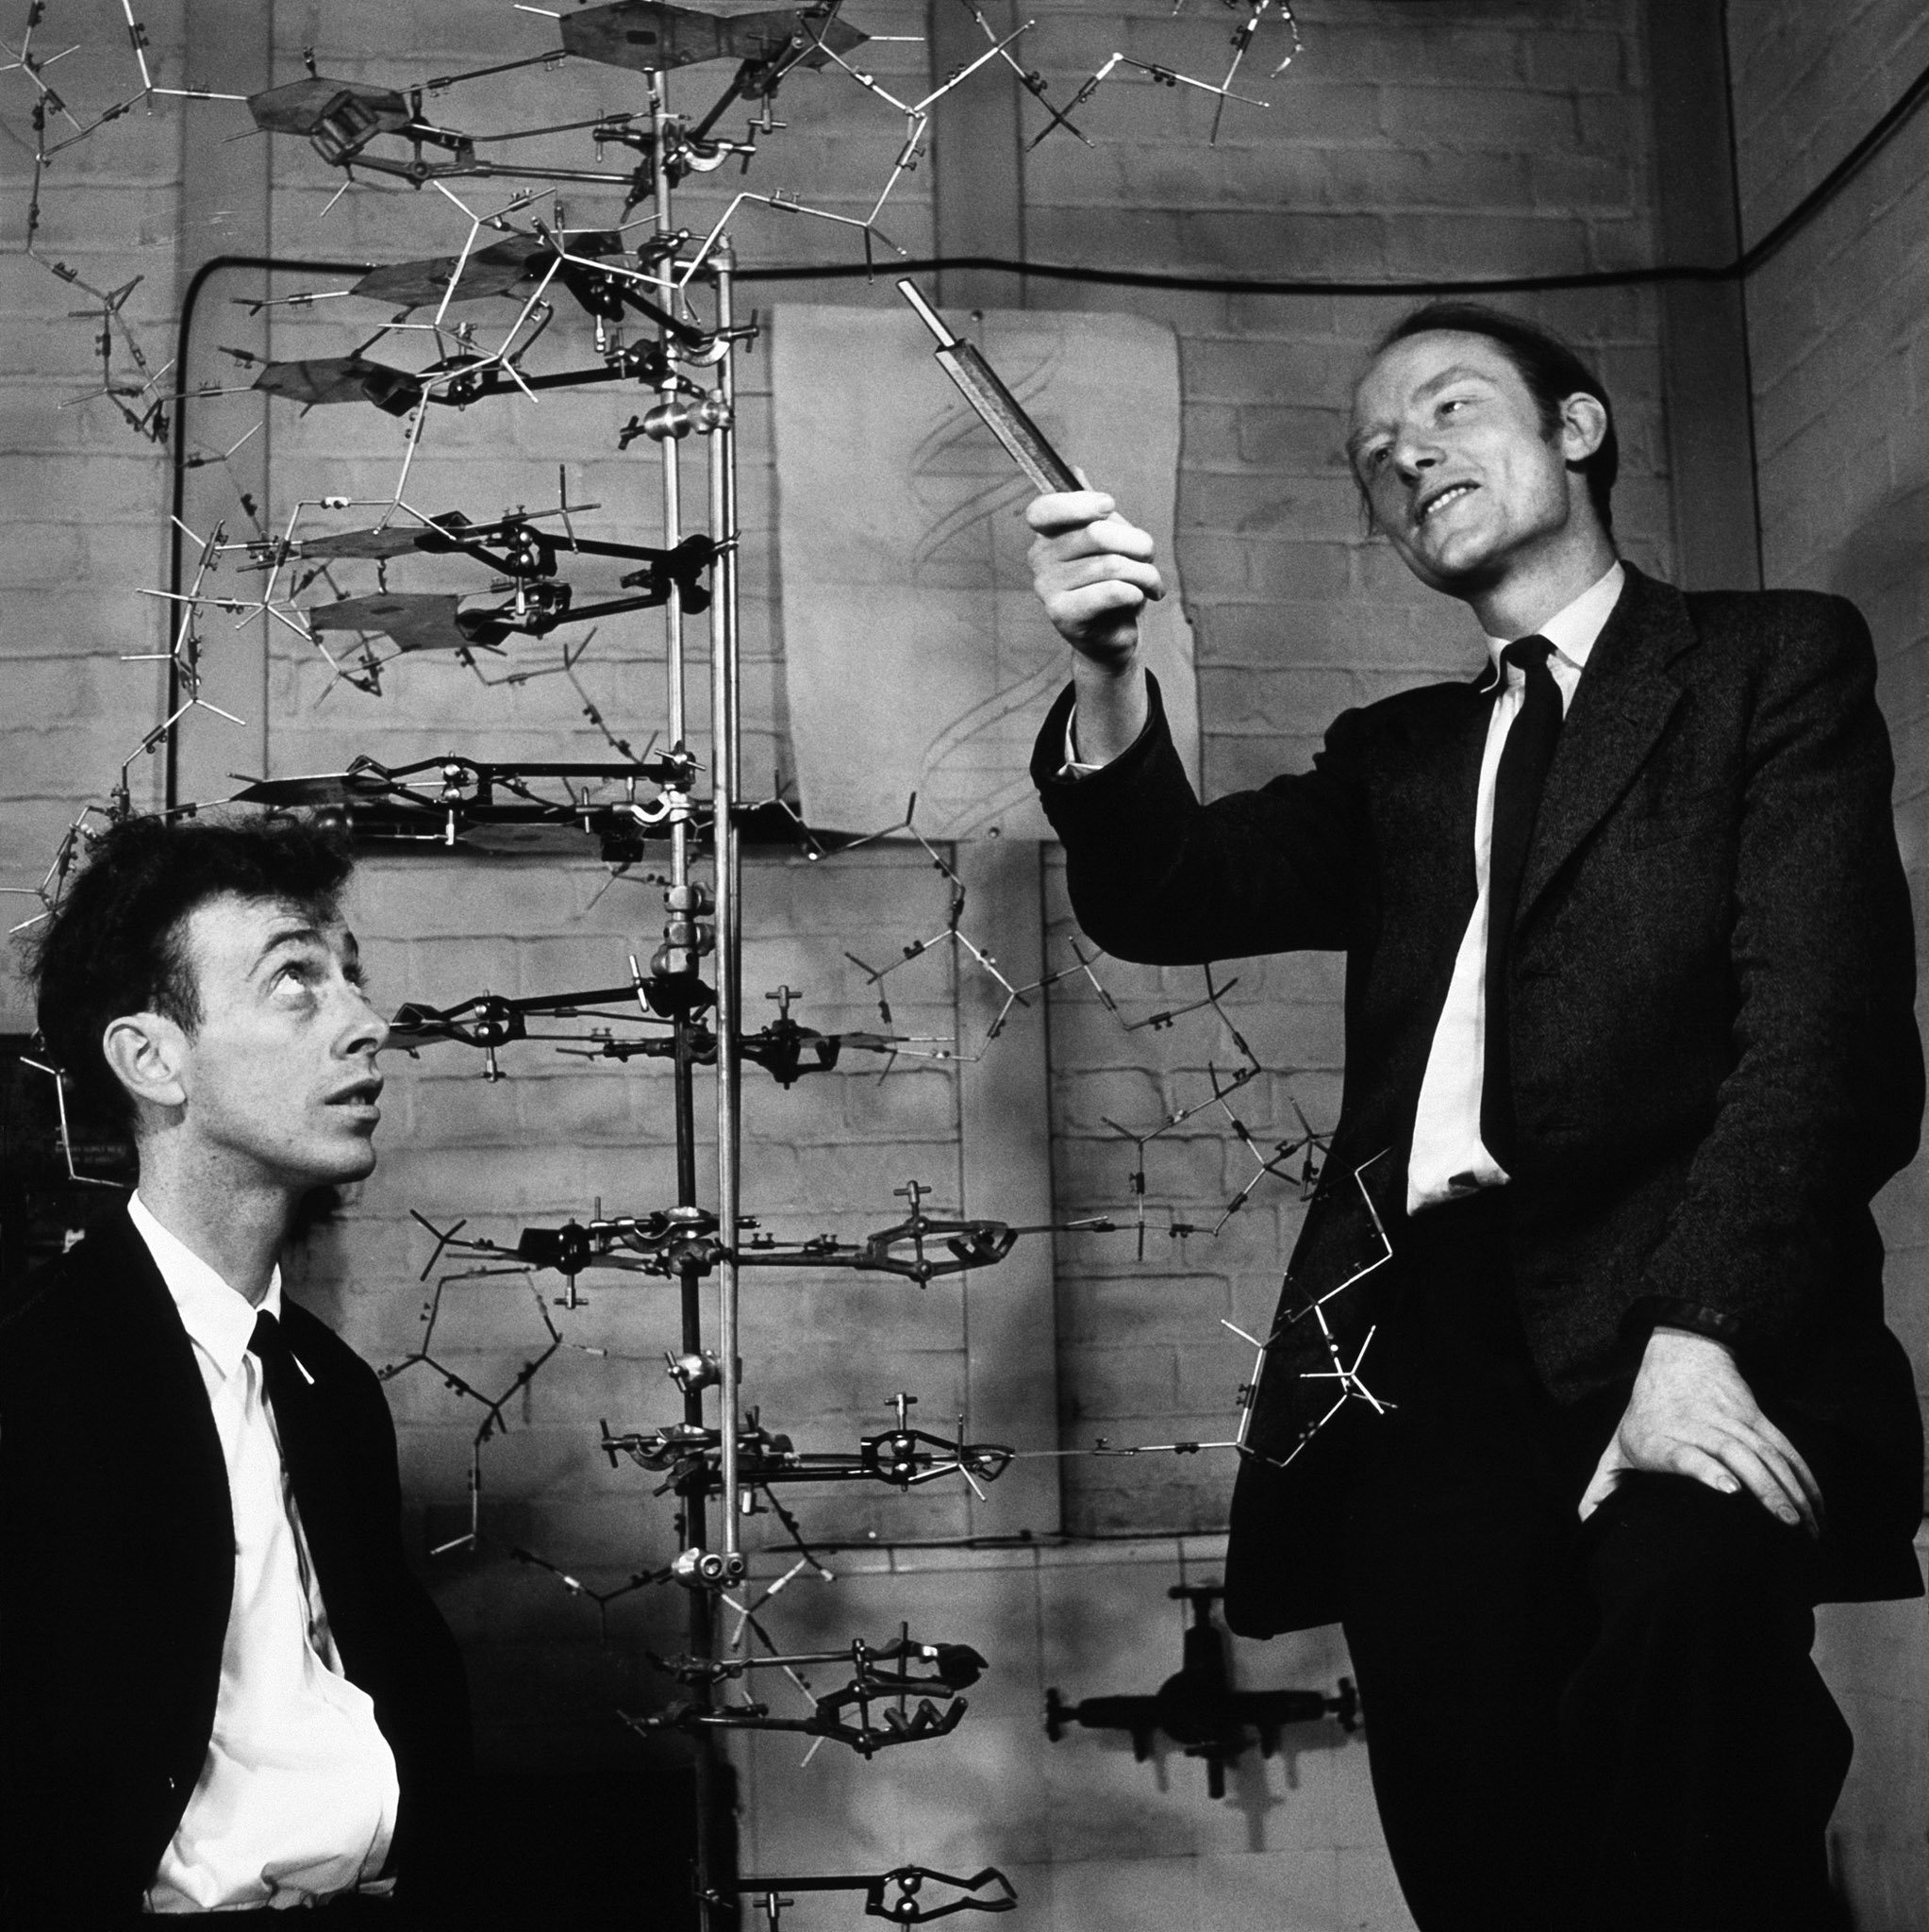
\includegraphics[width=0.5\linewidth]{./figures/ch1/watson_crick_dna_model}}
    \caption[Modèle physique de l'ADN par Watson et Crick.]{\it Modèle physique de l'ADN par Watson et Crick publiée en 1953 dans \textit{Nature}. Le modèle physique créé pour l'occasion est constitué de pièces en ferraille récupérées au sein de leur laboratoire.\footnote{\url{http://www.thehistoryblog.com/archives/25193}}}
    \label{Fig:watson_crick_dna_model}
\end{figure}

% \commentaire{MB: je peux me tromper, mais me semble que Watson et Crick avaient leur modele physique de l'ADN en 1953 deja; puis me demande si Pauling n'a pas utilise des modeles boules et batons en bois avant aussi. Donc l'info concernant Kendrew Perutz 1957 est a verifier}

La première représentation physique notoire d'une protéine est le fait de J.C. Kendrew qui, pour illustrer la résolution de la structure de la myoglobine par cristallographie \cite{kendrew1958three} à rayon X, a créé plusieurs modèles de cette structure. Il créa en collaboration avec Max Perutz le premier modèle, en 1957, composé exclusivement de plasticine (voir Figure \ref{Fig:kendrew_plasticine}). La qualité du modèle était en corrélation directe avec la résolution expérimentale de la structure cristallographique qui avait une basse résolution d'environ 6\r{A}, rapportant ainsi grossièrement la structure tertiaire mais pas davantage de la protéine. Ce modèle leur permis tout de même d'obtenir en 1962 le prix Nobel de chimie. Il fut le prédécesseur d'un autre modèle construit par les deux mêmes scientifiques et appelé \textit{forest of rods} (littéralement forêt de tiges), qui, avec une échelle de 5cm pour 1\r{A}, était composé de 2500 tiges verticales remplissant un cube de 2m de côté (voir Figure \ref{Fig:kendrew_myoglobin_forest_of_rods}). Des attaches de couleur étaient attachées aux tiges afin de représenter la densité d'électrons et guider la construction du modèle. Il fit suite à une amélioration de la résolution des cartes de densité de cristallographie atteignant 2\r{A} de précision. Les chaînes latérales n'étaient cependant pas encore bien discernables et il fallut attendre 1965 pour que les résultats expérimentaux permettent de construire un modèle plus précis. Pour ce faire, Kendrew approcha A.A Baker et ils mirent au point un modèle composé de balles et de bâtons afin de représenter les atomes et leurs liaisons (voir Figure \ref{Fig:kendrew_myoglobin_ball_and_spokes}). L'échelle de ces modèles était plus petite (entre 2.5 et 1cm / \r{A}) et rendait ces modèles plus facilement transportables mais cependant de taille encore conséquente. La construction de ces modèles se faisaient grâce à la projection des cartes de densités électroniques dessinées sur des plaques de verre dans un dispositif innovant appelé \textit{Richard's box} et illustrés dans la Figure \ref{Fig:fred_richards_ribonuclease}.

\begin{figure}
  \begin{subfigure}{.5\textwidth}
  \centering
  {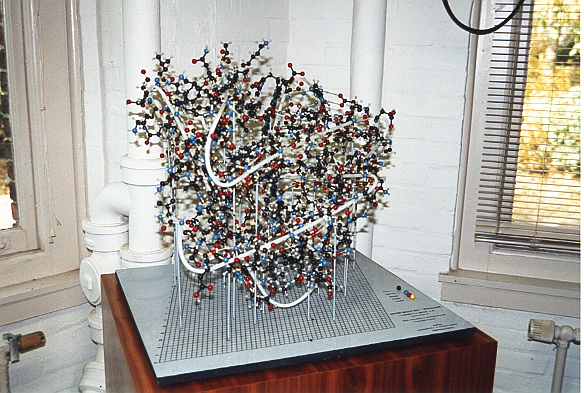
\includegraphics[height=5.5cm]{./figures/ch1/kendrew_myoglobin_ball_and_spokes}}
  \caption{}
    \label{Fig:kendrew_myoglobin_ball_and_spokes}
  % \hspace{0.2cm}
  \end{subfigure}%
  \begin{subfigure}{.5\textwidth}
  \centering
  {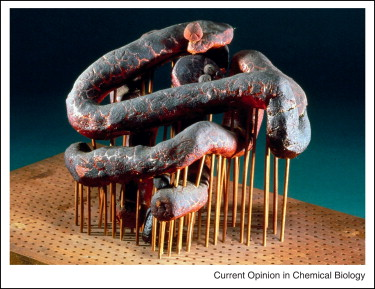
\includegraphics[height=5.5cm]{./figures/ch1/kendrew_myoglobin_plasticine}}
  \caption{}
  \label{Fig:kendrew_plasticine}
  % \hspace{0.2cm}
  \end{subfigure}%
  \\[\baselineskip]
  \begin{subfigure}{.5\textwidth}
  \centering
  {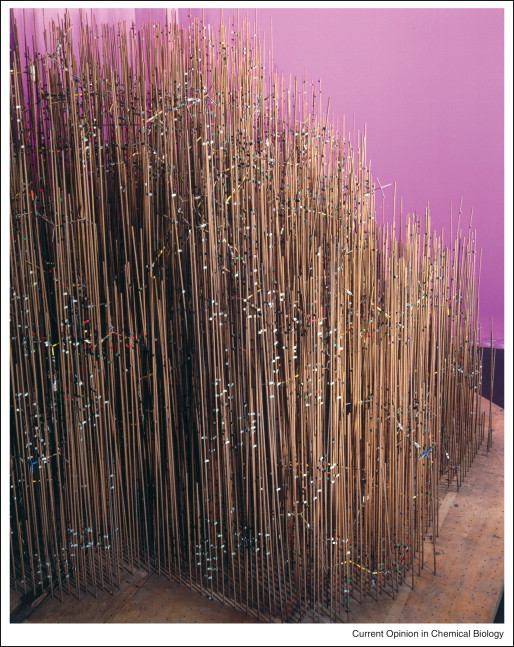
\includegraphics[height=9.5cm]{./figures/ch1/kendrew_myoglobin_forest_of_rods}}    
  \caption{}
  \label{Fig:kendrew_myoglobin_forest_of_rods}
  \end{subfigure}%
  \begin{subfigure}{.5\textwidth}
  \centering
  {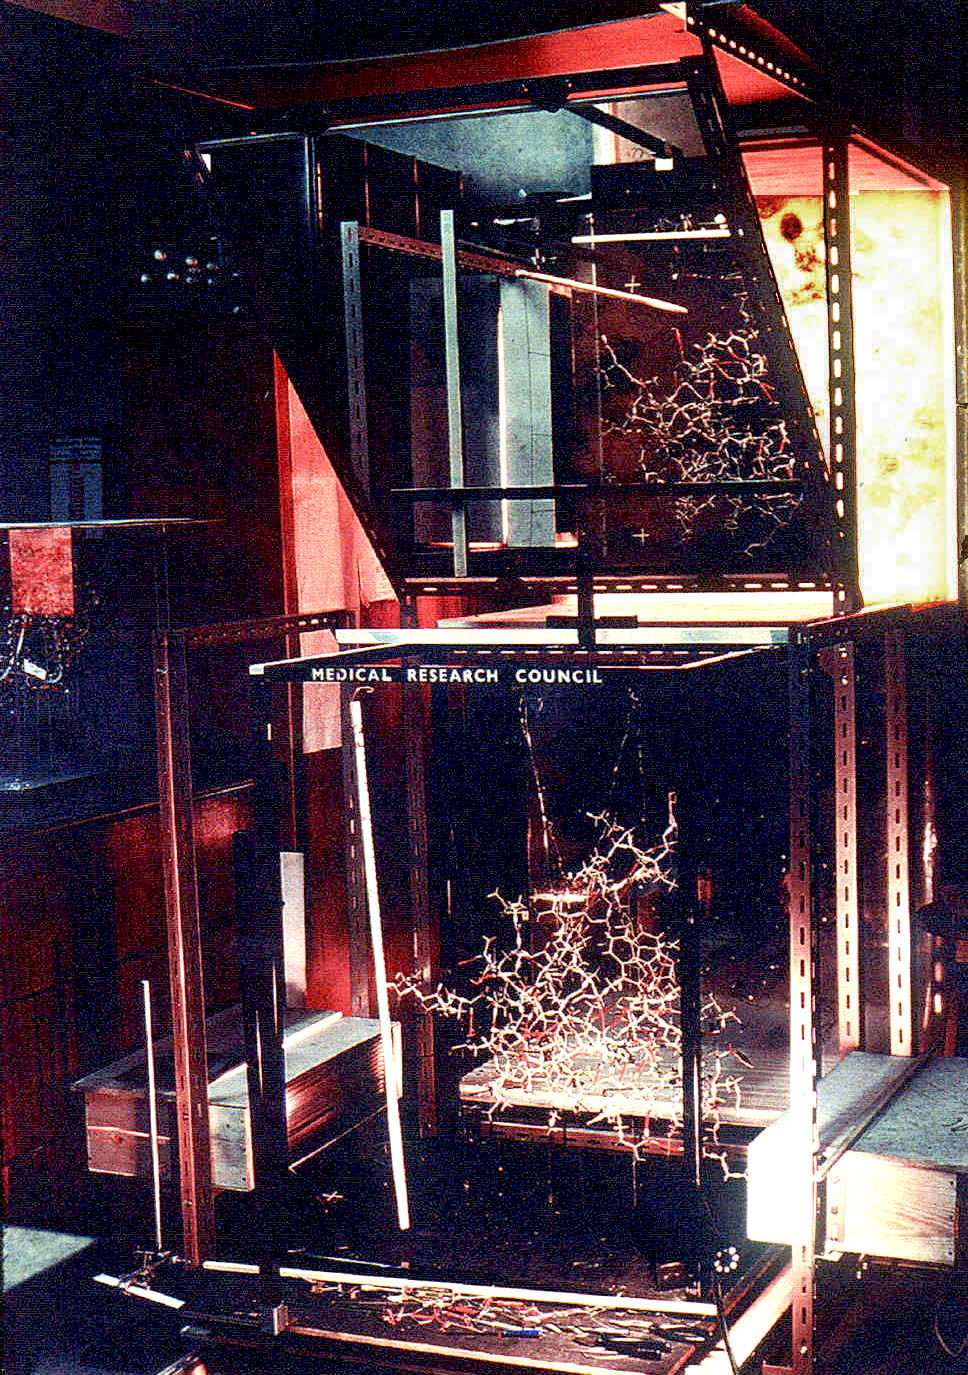
\includegraphics[height=9.5cm]{./figures/ch1/fred_richards_ribonuclease}}
  \caption{}
  \label{Fig:fred_richards_ribonuclease}
  \end{subfigure}%
  \caption[Différents modèles et techniques physiques de représentation de protéines.]{\it 
  (a) Modèle balle et bâtons représentant fois la myoglobine. Afin de mettre en évidence la chaîne principale, un fil blanc épais a été ajouté à l'ensemble et est la seule caractéristique vraiment discernable au milieu de tous les atomes (boules de couleur) et de leurs liaisons (bâtons).\footnote{\url{http://www.umass.edu/molvis/francoeur/barker/barker.html}}
  (b) Premier modèle physique de la myoglobine, conçu par Sir John Kendrew et Max Perutz. Ce modèle fut récompensé par le prix Nobel de chimie en 1962. Source : Science Museum/Science \& Society Picture Library
  (c) Modèle basé sur des tiges et des attaches de couleurs représentant également la myoglobine. Couramment appelé la <<forêt de tiges>> en français. Source : Science Museum/Science \& Society Picture Library
  (d) Dispositif de visualisation appelé <<Richards box>> (ou <<Fred's Folly>>) et permettant aux cristallographes de construire un modèle physique à partir d'empilements de feuillets représentant des cartes de densité électronique projetés à travers un miroir semi-argenté. Source : \cite{lim_frederic_2009}}
\end{figure}

Dans le début des années 1970, le cristallographe Byron Rubin mis au point une machine permettant de plier un câble selon la forme de la chaîne principale d'une protéine. Les modèles générés par cette machine, appelée \textit{Byron's Bender}, sont de plus petites tailles que les autres modèles physiques existants à cette époque là et permettait donc leur utilisation lors de réunions scientifiques. C'est d'ailleurs à l'occasion de l'une d'entre-elles, en 1976, alors que moins de deux douzaines de structures avaient été résolues, que deux modèles physiques de Bender représentant le fragment Fab de l'immunoglobuline et la dismutase superoxyde furent ramené par deux groupes distincts de chercheurs. Après comparaison des modèles, ils émirent l'hypothèse que ces deux protéines adoptaient probablement les mêmes méthodes de structuration malgré seulement 9\% d'identité de leurs séquences primaires \cite{richardson1976similarity}. Cet événement, pouvant être qualifier de hasard de l'histoire, fut la première reconnaissance de l'existence de la superfamille des domaines immunoglobulines non liés par leur séquence.

\begin{figure}
  \begin{subfigure}{.5\textwidth}
  \centering
  {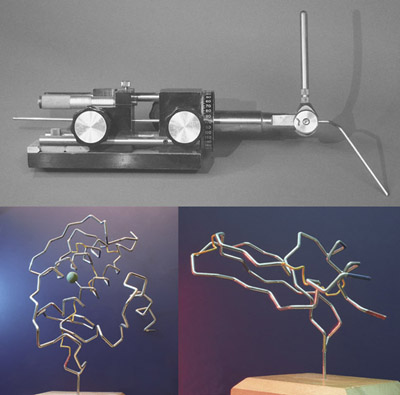
\includegraphics[height=6cm]{./figures/ch1/bender_tool_models}}
    \label{Fig:bender_tool_models}
  \caption{}
  % \hspace{0.2cm}
  \end{subfigure}%
  \begin{subfigure}{.5\textwidth}
  \centering
  {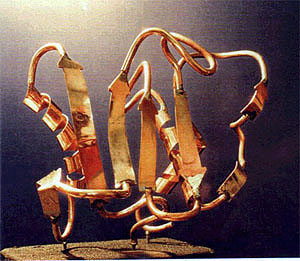
\includegraphics[height=6cm]{./figures/ch1/byron_sculpture_colagenase}}    
    \label{Fig:byron_rubin_art}
  \caption{}
  % \hspace{0.2cm}
  \end{subfigure}%
 \caption[(a) \textit{Byron's Bender} et plusieurs représentations physiques de protéines créées avec l'outil. (b) Sculpture moléculaire d'une collagénase de Byron Rubin.]{\it (a) En haut, l'outil mis au point par Byron Rubin permettant de plier une tige de métal suivant la structuration d'une chaîne principale de protéine. En dessous sont exposés les modèles de la phospholipase pancréatique A2 (à gauche) et de l'inhibiteur de la trypsine pancréatique bovine (à droite).\footnote{\url{http://jbiocommunication.org/issues/31-2/feature2.html}}
  (b) Sculpture moléculaire de Byron Rubin représentant une collagénase neutrophile humaine créée à partir d'une version plus grande de son Bender inspirée des outils de modelage automobiles locaux.\footnote{\url{http://www.umass.edu/microbio/rasmol/history.htm}}}
\end{figure}

Au-delà de l'importance de l'aspect tactile et visuel des modèles de \textit{Bender}, une autre facette importante de ces modèles est leur possibilité de vibrer au toucher, simulant ainsi le mouvement thermique. Cet aspect est d'importance quand comparée aux modèles virtuels qui font parfois oublier à leurs utilisateurs la flexibilité que possède une protéine dans son environnement cellulaire. 

Byron Rubin s'associa également, de façon plus étonnante, avec un garage de voitures local afin d'utiliser leur machine de pliage de pot d'échappement, fonctionnant sur le même principe que sa machine, afin d'atteindre une plus grande échelle. Il créa de nombreuses sculptures de molécules considérées comme importantes à partir de ce temps là et jusqu'aux années 90.

Concurrencés par les modèles sur ordinateurs, les modèles physique surent néanmoins évoluer avec les technologies, après le métal, le bois ou le plastique furent le support de plusieurs modèles. A la fin des années 90, grâce aux efforts de Michael Bauler et Tim Herman d'utiliser les nouvelles technologies d’ingénierie, les lasers et imprimantes 3D permirent la création de modèles à moindre coût et moindre temps ainsi qu'à une échelle toujours plus fine, plusieurs d'entre-eux sont représentés dans les Figures \ref{Fig:julian_wood_matingpheromone} et \ref{Fig:bathsheba_laser_dna}. L'ensemble de ces modèles prit une part importante dans l'éducation et voit maintenant plusieurs projets se servir de ces modèles comme interfaces tangibles pour des expériences de simulations moléculaires interactives permettant ainsi à l'utilisateur de conduire à travers une représentation physique de la molécule qu'il étudie \cite{gillet2005tangible}.


\begin{figure}
  \begin{subfigure}{.3\textwidth}
  \centering
  {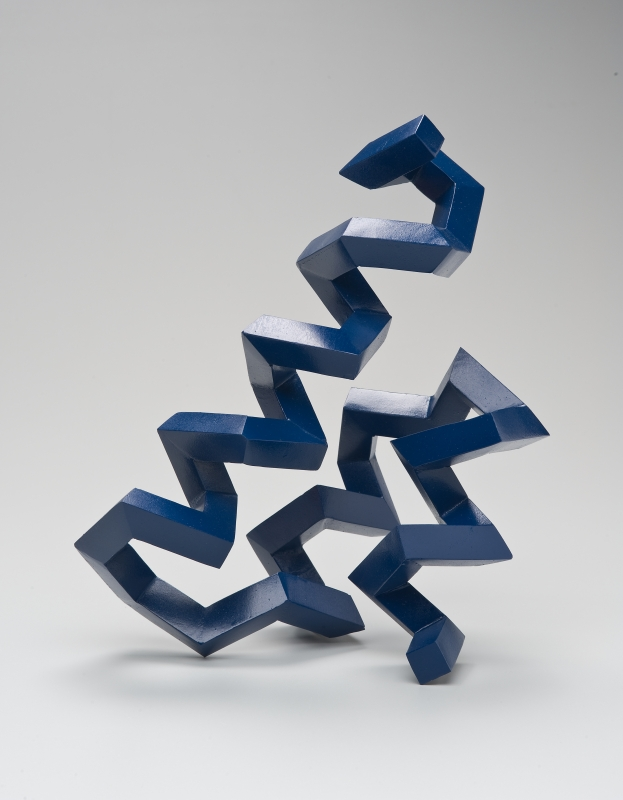
\includegraphics[width=0.9\linewidth]{./figures/ch1/julian_wood_matingpheromone}}
  \caption{}
  \label{Fig:julian_wood_matingpheromone}
  % \hspace{0.2cm}
  \end{subfigure}%
  \begin{subfigure}{.7\textwidth}
  \centering
  {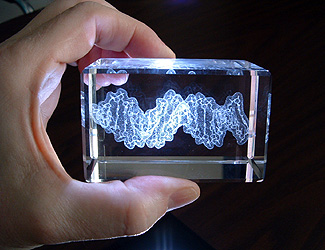
\includegraphics[width=0.9\linewidth]{./figures/ch1/bathsheba_laser_dna}}
  \caption{}
  \label{Fig:bathsheba_laser_dna}
  \hspace{0.2cm}
  \end{subfigure}%
 \caption[Modèles artistiques d'une phéromone et d'un brin d'ADN.]{\it (a) Modèle en bois de Julian Voss-Andreae illustrant la chaîne principale d'une phéromone.\footnote{\url{http://julianvossandreae.com/works/protein-sculptures-indoor-works/}}
  (b) Modèle en verre de l'ADN creusé grâce à des rayons lasers fins.\footnote{\url{http://www.umass.edu/microbio/rasmol/history.htm}}}
\end{figure}


\myparagraph{Représentations \textit{in silico}}

Les premiers modèles de structures moléculaires réalisés sur ordinateurs ne sont pas vraiment postérieurs aux premiers modèles physiques que nous avons cité. En effet, c'est en 1964 que Cyrus Levinthal et ses collègues du MIT ont développé un système qui permettait d'afficher, sur un oscilloscope, une représentation filaire d'une structure macromoléculaire (voir Figure \ref{Fig:levinthal_oscilloscope_wireframe}).
En 1965, Carroll K. Jonhson publia un programme créé en Fortran et appelé \textbf{ORTEP} (\textit{Oak Ridge Thermal Ellipsoid Plot Program}) permettant de générer des illustrations de structures. Les cristallographes l'adoptèrent rapidement et s'en servirent pour publier leurs structures lors de conférences ou au sein d'articles de journaux. Sa capacité à générer des images stéréoscopiques des structures fut l'une des grandes forces d'ORTEP qui a vu sa seconde version être sortie en 1976 et sa troisième en 1996, cette dernière étant toujours disponible à l'utilisation\footnote{\url{http://web.ornl.gov/sci/ortep/}}. ORTEP fut notamment utilisé pour illustrer la structure de la myoglobine et ces illustrations firent écho auprès de John C. Kendrew qui félicita personnellement Carroll K. Johnson pour son travail (voir Figure \ref{Fig:ortep_myoglobin}).

\begin{figure}
  \begin{subfigure}{.5\textwidth}
  \centering
  {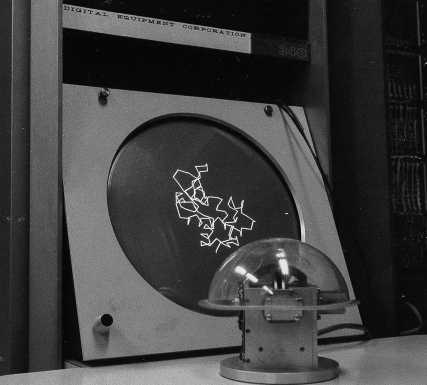
\includegraphics[width=0.9\linewidth]{./figures/ch1/levinthal_oscilloscope_wireframe}}
  \caption{}
  \label{Fig:levinthal_oscilloscope_wireframe}
  % \hspace{0.2cm}
  \end{subfigure}%
  \begin{subfigure}{.5\textwidth}
  \centering
  {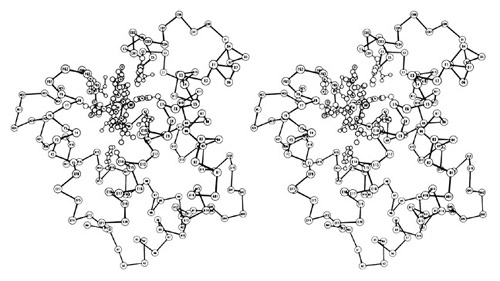
\includegraphics[width=0.9\linewidth]{./figures/ch1/ortep_myoglobin}}    
  \caption{}
  \label{Fig:ortep_myoglobin}
  \hspace{0.2cm}
  \end{subfigure}%
 \caption[(a) Premier système d'ordinateur pour visualiser des molécules développé par Cyrus Levinthal. (b) Vue stéréoscopique d'un dessin du squelette de la myoglobine générée par ORTEP.]{\it (a) Le premier système d'ordinateur pour visualiser des molécules développé par Cyrus Levinthal au sein du Massachussetts Institute of Technology (MIT) en 1962. Un simple modèle de squelette moléculaire esst visible sur l'écran de l'oscilloscope. En bougeant le globe plastique au premier plan, il était possible de faire tourner le modèle à l'écran.\footnote{\url{http://www.umass.edu/microbio/rasmol/history.htm}}
  (b) Vue stéréoscopique d'un dessin du squelette de la myoglobine générée par ORTEP.\footnote{\url{http://jbiocommunication.org/issues/31-2/feature2.html}}}
\end{figure}

A ce moment là, les ordinateurs n'étaient pas encore capables d'interpréter seuls les coordonnées obtenues par cristallographie et il était nécessaire de construire un modèle de Kendrew, d'en mesurer les liaisons, avant de les rentrer dans l'ordinateur pour générer une représentation virtuelle.

Cela changea au milieu des années 70 quand, pour la première fois, une structure obtenue par cristallographie fut résolue et visualisée uniquement par des ordinateurs sans qu'un modèle physique existe. Pour ce faire, David et Jane Richardson utilisèrent un ordinateur permettant d'ajuster directement la densité électronique afin de générer un modèle virtuel de la structure d'une superoxyde dismutase \cite{tainer1982determination}. Ce système informatique, appelé \textbf{GRIP} fut le prédécesseur de plusieurs programmes permettant ce passage d'une carte de densité électronique à une structure 3d moléculaire sur ordinateur (voir Figure \ref{Fig:richardson_grip_computer}). Parmi ces programmes, en 1974 le laboratoire de biographie à l'université A\&M du Texas développèrent un programme appelé \textbf{FIT} permettant de résoudre la structure de la nucléase \textit{Staphylococcus} \cite{collins1975protein}. A la fin des années 70, le programme \textbf{FRODO} fut publié par T. Alwyn Jones et devint l'outil standard pour construire des modèles virtuels à partir de cartes de densité électronique \cite{jones1978graphics}. Il est même estimé que 95\% des structures cristallographiques résolues depuis le début des années 80 ont été construites en utilisant FRODO ou son successeur <<O>>. Il permet une interaction de l'utilisateur avec le modèle en proposant de le tourner selon les trois axes de rotation X, Y et Z.

\begin{figure}
  \begin{subfigure}{.5\textwidth}
  \centering
  {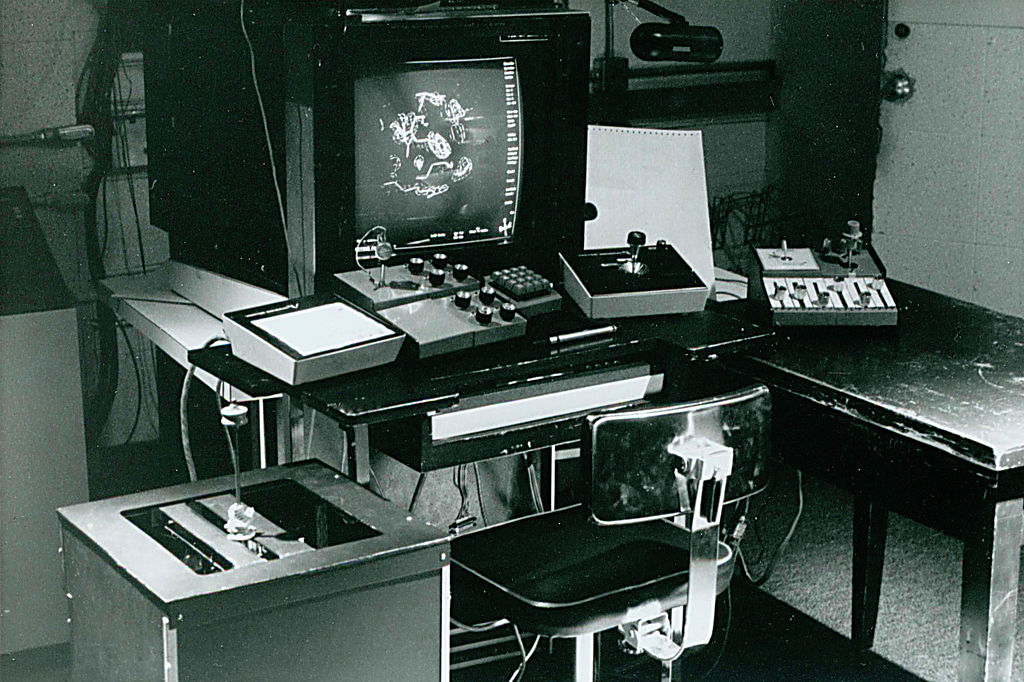
\includegraphics[width=0.9\linewidth]{./figures/ch1/richardson_grip_computer}}
  \caption{}
  \label{Fig:richardson_grip_computer}
  % \hspace{0.2cm}
  \end{subfigure}%
  \begin{subfigure}{.5\textwidth}
  \centering
  {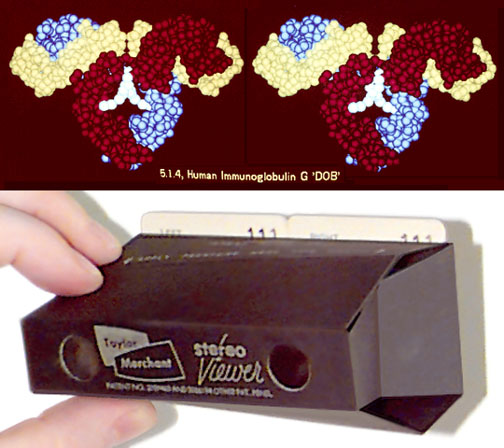
\includegraphics[width=0.9\linewidth]{./figures/ch1/TAMS_viewer_slide}}    
  \caption{}
  \label{Fig:TAMS_viewer_slide}
  % \hspace{0.2cm}
  \end{subfigure}%
 \caption[]{\it (a) Système d'ordinateur GRIP créé par David et Jane Richardson permettant d'ajuster une carte de densité électronique pour créer un modèle virtuel. Source : \cite{jslipscomb_english:_1981}
  (b) En haut, exemple d'une des 116 vignettes présentes dans le set TAMS et permettant la vue stéréoscopique d'une immunoglobuline humaine grâce à un visualiseur de poche pliable (en bas).\footnote{\url{http://jbiocommunication.org/issues/31-2/feature2.html}}}
\end{figure}

A la fin des années 70, de plus en plus de cristallographes franchirent le pas de la construction de modèles de nouvelles protéines résolues non plus par modèles physiques mais grâce à des modèles par ordinateur. L'un des principaux avantages de ces derniers est la possibilité de garder en mémoire les coordonnées atomiques alors que lors de l'utilisation de modèles de Kendrew, elles devaient être mesurées à la main, atome par atome. En 1977, un atlas des structures macromoléculaires sous forme filaire fut publié. A la fin des années 70, Thomas K. Porter mis au point des algorithmes de représentations volumiques avec ombres. Cela révolutionna la représentation des molécules mais n'était accessible qu'à un nombre limité de spécialistes possédant les plus puissants ordinateurs de l'époque.
Le National Institutes of Health (NIH), qui employait Thomas K. Porter à l'époque, trouva cependant trop onéreux la publication d'un atlas de représentations volumiques de structures moléculaires en couleur. Leur idée de publication fut cependant de nouveau d'actualité quand ils prirent connaissance de l'existance d'un lecteur de carte pour vignettes stéréoscopiques à moindre coût. Ce visualiseur en carton pouvait se plier et possédait donc un avantage certain pour la distribution de 116 vignettes, éditées par Richard Feldman grâce aux algorithmes de rendu volumique. Ce set de vignettes fut appelée TAMS pour \textit{Teaching Aids for Macromolecular Structure}. Parmi les vignettes, plusieurs représentations étaient utilisées et plusieurs informations structurelles pouvaient être représentées, incluant un paragraphe d'explication associé. Un exemple de vignette est présenté dans la Figure \ref{Fig:TAMS_viewer_slide}.


Jusqu'au début des années 90, l'utilisation de programmes de visualisation était exclusivement associée à des ordinateurs particuliers financièrement peu abordables et accessibles à une partie seulement des chercheurs. Cela changea en 1992 quand David et Jane Richardson décrirent le format \textit{kinemage} et leurs deux programmes associés \textbf{MAGE} et \textbf{PREKIN} \cite{richardson1992kinemage}. Grâce à leur implémentation sur Macintosh, il fut le premier programme à pouvoir être utilisé par une large communauté de scientifiques, d'enseignants et d'étudiants. Le format \textit{kinemage} permettait aux utilisateurs de générer une image animée de la structure ou sous-partie de structure qu'ils voulaient mettre en avant. Se rapprochant d'un GIF animé et bien qu'ayant disposé d'une grande popularité, en particulier en fournissant plus d'un millier d'illustrations pour les articles de \textit{Protein Science}, il manquait à ce format la possibilité de diriger l'exploration d'une structure de façon neutre et interactive.

Ce manque fut comblé par RasMol en 1993. Ce programme fut la continuité d'un premier programme développé par Roger Sayle en 1989 et permettant le \textit{shadowing} (ombrage en français) rapide d'objets virtuels permettant leur rotation en temps réel. 
Avec le mentorat d'un cristallographe, Andrew Coulson appliqua son algorithme sur des structures moléculaires et publia en 1992 une suite logicielle complète de visualisation moléculaire appelée \textbf{RasMol} possédant, entre autres, un nombre important de paramètres de rendus graphiques (rendu volumique, réflectivité des surfaces, etc) et une interface graphique soignée \cite{sayle1992rasmol}. Les sources en C de ce programme furent rapidement mis à disposition de la communauté par Roger Sayle à l'obtention de son doctorat et put ainsi être adapté pour de multiples plateformes. Dés 1993 de nombreuses illustrations scientifiques s'appuyaient sur RasMol et les enseignants en ont rapidement fait également un outil de choix. Preuve de sa popularité, on estimait en 2005 le nombre d'utilisateurs à plus d'un million à travers le monde \cite{martz2004history}.

L'avènement du web fit apparaître quelques années plus tard un programme basé sur le portage du code C de RasMol vers C++. Développé par Bryan van Vliet et Tim Maffett, \textbf{Chime} (pour CHemical mIME) fut publié sous forme de plug-in pour le navigateur web Netscape. La possibilité d'associer cet espace de visualisation à des contenus web et de télécharger des modèles depuis des bases de données en ligne furent deux des principales raisons de son succès, en particulier dans le milieu académique et éducatif. Plusieurs centaines de tutoriels furent publiés sur le web en utilisant Chime et servirent de support à des étudiants mais également à des cristallographes experts. Ses applications furent donc à la fois la communication de structures à travers le web mais également la diffusion des connaissances et le support d'apprentissage.


\subsubsection{La visualisation moléculaire contemporaine}

Les programmes de visualisation moléculaire 3d permettent d'observer, dans un espace graphique 3d virtuel, des représentations abstraites de molécules à partir de fichiers de leurs coordonnées 3d. Ces coordonnées 3d sont communément inscrites dans des fichiers PDB (format provenant de la base de données \textit{Protein Data Bank} fournissant un standard pour la représentation des données de structures macromolécules dérivées de RMN ou cristallographie\footnote{\url{http://www.rcsb.org/pdb/static.do?p=file_formats/pdb/index.html}}).

Les logiciels de visualisation permettent principalement de mettre en avant certaines des particularités structurelles des molécules au moyen de jeux de couleurs ou de formes plus ou moins adoptés dans la communauté. Il est compliqué de parler de standards sans un consensus officiel clair, n'existant pas actuellement, et plusieurs initiatives cherchent encore à faire évoluer les méthodes de représentation graphiques. Cependant, un certain accord s'est trouvé quant au jeu des couleurs et le schéma de couleur CPK (Corey-Pauling-Koltun) est certainement le schéma le plus utilisé \cite{corey1953molecular}.

Ces programmes s'appuient sur différents formats de fichier pour ces coordonnées même si la plupart sont capables de lire au moins le format PDB. Au-delà de la visualisation statique de structures 3d, il est souvent possible d'utiliser ces programmes afin de lire la trajectoire d'une simulation numérique. Ainsi, il est possible d'observer l'évolution structurelle d'un complexe moléculaire au cours du temps ou d'observer des phénomènes biologiques (passage de molécules au travers d'une membrane, repliement d'une région protéique suite à son interaction avec un partenaire biologique, etc.). Parmi les programmes de visualisation 3d largement utilisés aujourd'hui nous pouvons citer : 
\begin{itemize}
  \item \textbf{PyMol} \cite{delano_pymol_2002}, basé sur le langage Python et offrant une API pour ce langage, il dispose de nombreux rendus visuels et est, selon l'auteur original, utilisé dans plus d'un quart des images de structures moléculaires présentes dans les articles scientifiques. Il s'appuie sur la génération d'images de haute qualité grâce à des techniques de lancer de rayons. Son utilisation comme API est particulièrement adaptée au portage au sein de plateformes multi-composantes et il est la base de plusieurs travaux de l'équipe pour la visualisation moléculaire dans différents environnements immersifs.
  \item \textbf{VMD} \cite{humphrey_vmd:_1996}, spécialisé dans la visualisation et l'analyse de résultats de simulations de dynamiques moléculaires, cet outil est très usité du fait de ses nombreuses extensions et la possibilité de le relier à NAMD, un programme de dynamique moléculaire, permettant ainsi d'effectuer des simulations moléculaires interactives. Il est de plus bien adapté au rendu temps réel de larges modèles moléculaires grâce à des méthodes de rendus graphiques directement effectués et optimisés sur GPU.
  \item \textbf{Jmol} \cite{herraez2006biomolecules}, basé sur Java et disponible sous forme d'application indépendante ou intégrée dans des pages web, ce visualiseur est populaire du fait de sa facile intégration au sein de contenus web. Il offre de plus plusieurs rendus graphiques très performants.
  \item \textbf{YASARA} \cite{krieger2014yasara}, suite logicielle permettant à la fois la visualisation, mais aussi l’exécution de simulations moléculaires interactives, YASARA est depuis sa création dédiée pour le rendu stéréoscopique 3d et l'implication de l'utilisateur dans le suivi de sa simulation offrant même des solutions pour diriger la simulation en y ajoutant des forces.
  \item \textbf{SweetUnityMol} \cite{perez2015three}, est une extension de UnityMol \cite{lv2013game}, lui même utilisé comme base d'une partie de nos travaux, et s'intéresse plus particulièrement aux représentations 3d des glucides et des polysaccharides. Il utilise différentes méthodes de représentation acceptées au sein de la communauté scientifique des glycosciences et propose de nouvelles techniques de rendus graphiques.
\end{itemize}
% \commentaire{MB: j'ajouterai a la liste precedente aussi SweetUnityMol en indiquant que cela emane du laboratoire du co-directeur de these et formera une base pour une partie du travail de these; de maniere generale je trouve bien de nouver des ponts entre les chapitres introductives et le coeur de these decrit dans les chapitres ulterieurs}

Cette liste est non-exhaustive, mais recense quatre des logiciels de visualisation moléculaire les plus utilisés dans le monde scientifique et plus particulièrement en biologie structurale.

Ces programmes sont donc tous capables de représenter des modèles 3d de protéines grâce aux standards de représentation mis au point à travers les années. Parmi ceux-ci, il est possible d'extraire 7 modes de représentations souvent utilisés par la communauté de biologie structurale, à la fois dans leur travail quotidien, mais également au travers de leurs communications (conférences, articles, etc.).

\begin{figure}
  \begin{subfigure}{.5\textwidth}
  \centering
  {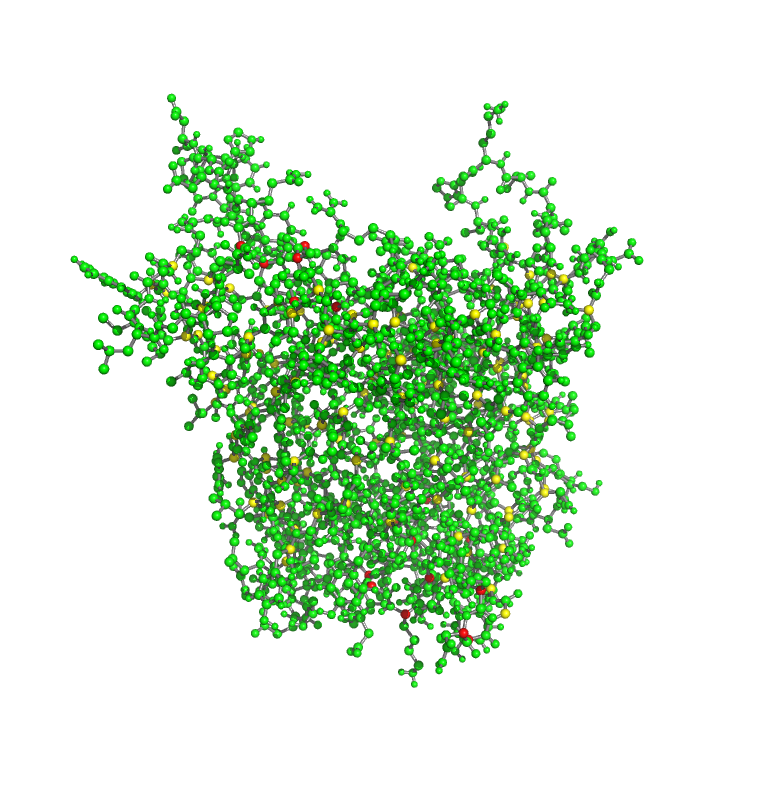
\includegraphics[width=\linewidth]{./figures/ch1/ball_sticks_representation}}
    \label{Fig:ball_sticks_representation}
  \caption{}
  % \hspace{0.2cm}
  \end{subfigure}%
  \begin{subfigure}{.5\textwidth}
  \centering
  {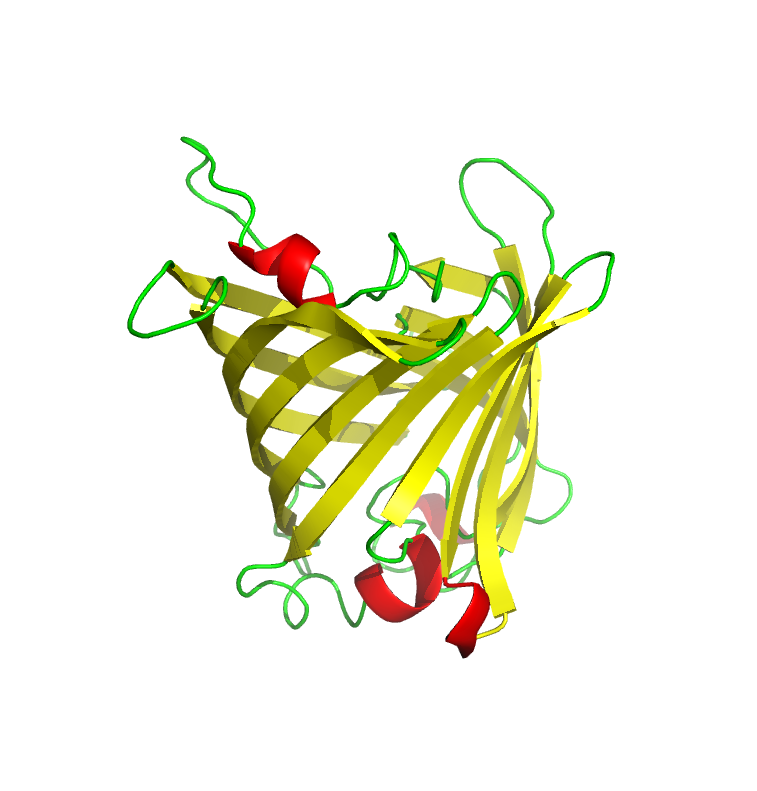
\includegraphics[width=\linewidth]{./figures/ch1/cartoon_representation}}    
    \label{Fig:cartoon_representation}
  \caption{}
  % \hspace{0.2cm}
  \end{subfigure}%
  \\[\baselineskip]
  \begin{subfigure}{.5\textwidth}
  \centering
  {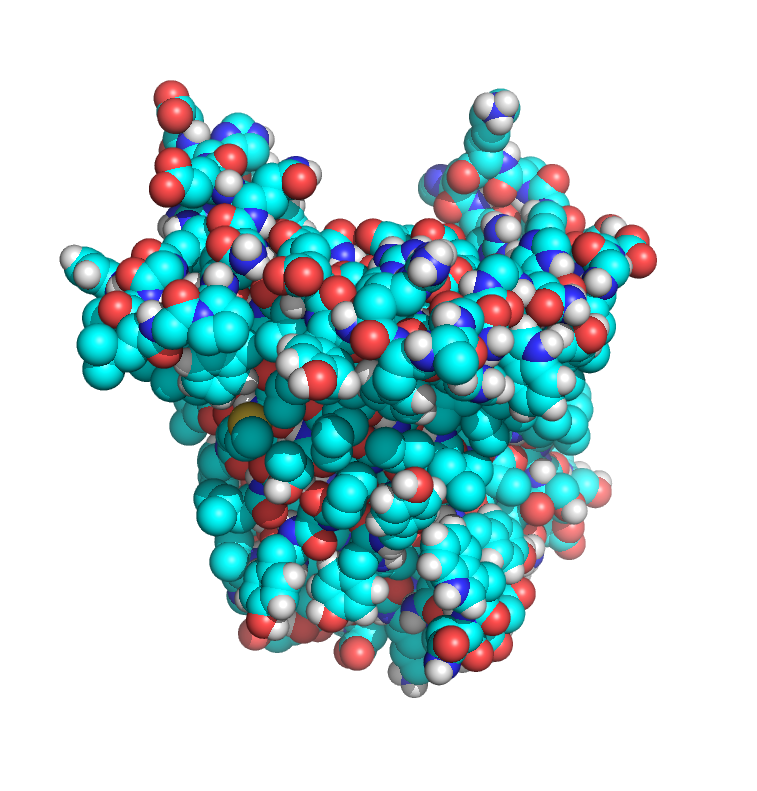
\includegraphics[width=\linewidth]{./figures/ch1/vdw_representation}}
  \caption{}
    \label{Fig:vdw_representation}
  % \hspace{0.2cm}
  \end{subfigure}%
  \begin{subfigure}{.5\textwidth}
  \centering
  {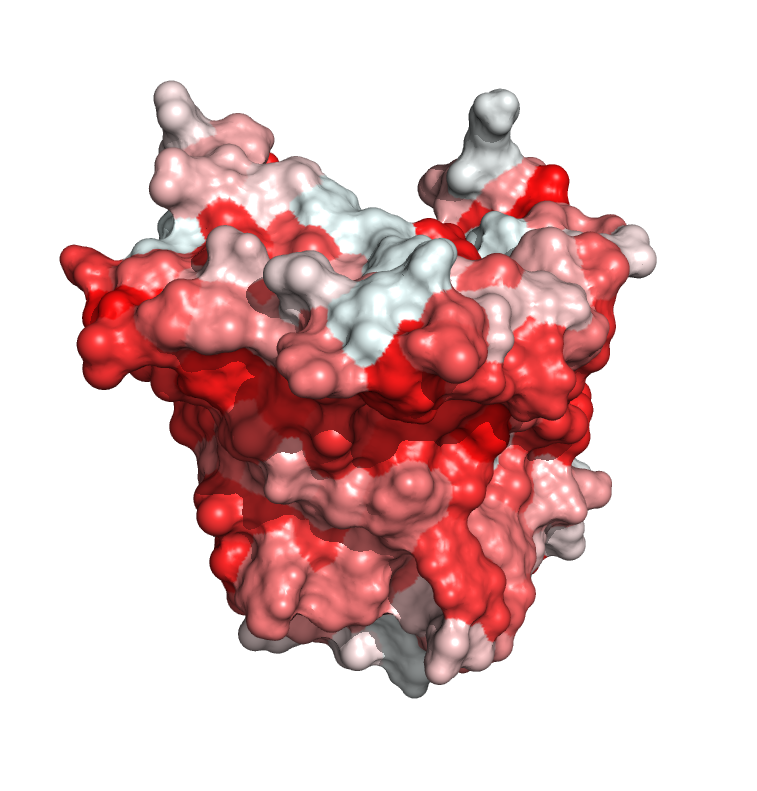
\includegraphics[width=\linewidth]{./figures/ch1/surface_representation}}
  \caption{}
    \label{Fig:surface_representation}
  % \hspace{0.2cm}
  \end{subfigure}%
  \caption[Différentes représentations informatiques de la protéine OMPLA par PyMol.]{\it Différentes représentations obtenues avec PyMol de la protéine OMPLA (pour \textit{Outer Membrane PhosphoLipase A}) enzyme présente à la surface de certaines bactéries. Elle est successivement représentée : (a) par balles et bâtons pour respectivement les atomes et leurs liaisons covalentes, (b) \textit{cartoon} permettant de mettre en avant une structuration en \textit{tonneaux bêta}, (c) sphères dont le rayon correspond aux rayons de van der Waals des atomes et (d) représentation surfacique dont le code couleur correspond à l'échelle d'hydrophobie des acides aminés présents à la surface.
  }
\end{figure}

\begin{itemize}
  \item Représentation par \textbf{ligne} : seules les liaisons covalentes entre atomes sont représentées par une ligne de longueur équivalente à la distance entre les deux centres des atomes situés de part et d'autre de la liaison. Cette représentation est souvent associée à une coloration précise, chacune de ses moitiés étant colorée de la couleur associée au type d'atome qu'elle relie.
  \item Représentation par \textbf{trace} : seule la chaîne principale de la protéine est représentée dans ce mode, par des bâtons droits dont les extrémités correspondent au centre d'un atome qu'elles relient.
  \item Représentation par \textbf{balles et bâtons} : alors que les atomes sont représentés par des sphères, les liaisons covalentes sont des bâtons. C'est l'une des représentations les plus courantes, car simple et permettant de rapidement cerner l'agencement d'atomes d'une même molécule. Elle est cependant plus adaptée aux molécules de tailles limitées, car elle engrange rapidement une surcharge visuelle pour les molécules de plus grande taille.
  \item Représentation par \textbf{rubans} : de la même manière que la représentation par trace, cette représentation suit les carbones alpha composant la chaîne principale de la protéine et affiche un ruban large le long de la chaîne principale.
  \item Représentation par \textit{\textbf{cartoon}}: ici, les différentes structurations composant la structure secondaire d'une protéine : hélices, feuillets et coudes, sont mises en avant respectivement par un ruban enroulé le long du squelette de la protéine, une flèche large pointant dans la direction du feuillet identifié et enfin un tube pour les coudes et boucles de la protéine rassemblant les parties non structurées.
  \item Représentation par \textbf{sphères} : chaque atome est représenté par une sphère dont le rayon est égal au rayon de Van der Waals de l'atome.
  \item Représentation par \textbf{surface} : dans ce mode, la SAS est représentée par une couche uniforme autour de la protéine.
\end{itemize}

Chaque type de représentation répond à des besoins de visualisation différents. Alors que l'agencement de la structure secondaire et tertiaire pourra être rapidement visualisé avec une représentation par \textit{cartoon}, il sera nécessaire d'ajouter une représentation par lignes afin d'observer la proximité des atomes entre eux. De la même façon, la détection visuelle des trous et potentiels sites de liaisons de la protéine sera facilitée par la représentation surfacique, mais le cœur de la protéine ne pourra être visualisé correctement qu'avec des représentations par ligne ou rubans. Ces différentes représentations ne sont pas cloisonnées et il n'est pas rare de les combiner afin de visualiser les caractéristiques propres à chaque représentation en même temps. Les calculs permettant chacune de ces représentations ne demandent pas les mêmes ressources computationnelles et même si la majorité d'entre elles peuvent aujourd'hui être appliquées de façon presque instantanée sur des ordinateurs de bureau, certaines comme la représentation par surface demandent des calculs coûteux sur des protéines de grande taille.

La représentation de surface fait justement partie des techniques de visualisation ayant pu profiter des avancées rapides provenant de certains domaines non scientifiques comme le jeu vidéo ou le cinéma. Certains rendus appelés \textit{photo-réalistes} et inspirés de techniques d'animation récentes sont maintenant retrouvés au sein de logiciels de visualisation de données scientifiques, améliorant sensiblement la perception des utilisateurs vis-à-vis de leurs données. La visualisation moléculaire n'a pas échappé à ces nouvelles techniques de rendus et a su implémenter certaines approches basées sur la \textbf{transparence}, les rendus \textbf{lumineux}, les effets de \textbf{profondeur}, etc. au sein des logiciels les plus utilisés dans la communauté. Ces nouvelles façons de représenter des structures protéiques permettent de jouer sur les capacités cognitives et perceptuelles des utilisateurs. Parallèlement, ces développements demandant des ressources computationnelles bien plus importantes que les anciennes implémentations graphiques, il a fallu également franchir le pas du calcul graphique sur GPU \cite{chavent_gpu-powered_2011}. La parallélisation des programmes et leur utilisation des ressources graphiques présentes au sein des ordinateurs ont permis de conserver des performances d'affichages suffisantes pour afficher des molécules de taille raisonnable. Dans cette même dynamique, certains projets s'appuient sur l'utilisation de moteurs de jeux vidéos pour développer des environnements de visualisation profitant des derniers progrès du domaine, dont la spécialisation et l'investissement associé dépassent de loin les moyens attribués à la seule visualisation moléculaire dans le monde de la science \cite{andrei2012intuitive,lv_game_2013}. Ces moteurs de jeu ouvrent de nouvelles perspectives pour la visualisation, mais également l'exploration des structures de protéines.

% \begin{figure}
%   \centering
%   {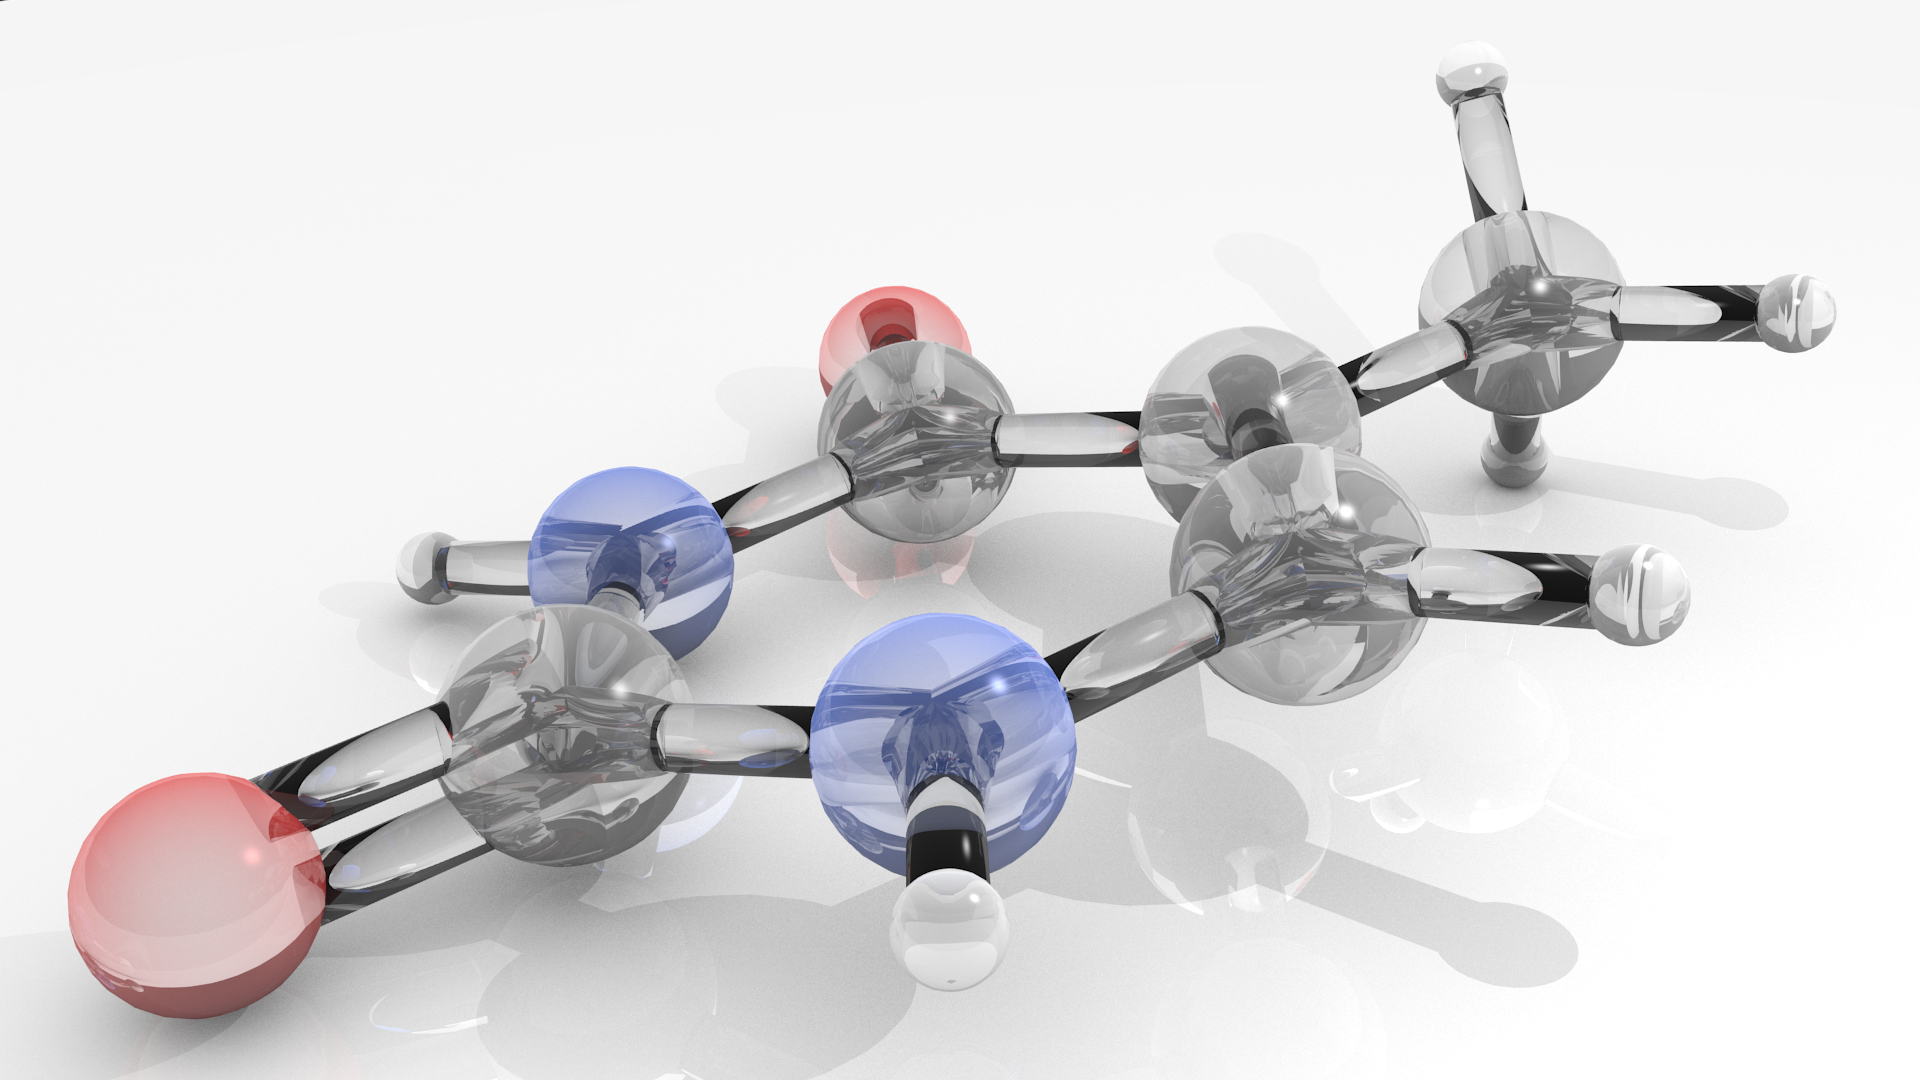
\includegraphics[width=.75\linewidth]{./figures/ch2/molecule_blender_glass}}
%     \caption{{\it Représentation}}
%   \label{Fig:molecule_blender_glass}
%   \hspace{0.2cm}
% \end{figure}


\subsubsection{Perspectives de la visualisation moléculaire}

La présence de GPUs performants sur une grande partie du parc informatique scientifique permet d'envisager sérieusement leur utilisation intensive pour le développement d'outils de visualisation performants. La prochaine grande étape est la mise à l'échelle de ces outils pour répondre aux enjeux de taille, au sens propre comme au figuré, inhérents aux structures étudiées. Nous avons vu que ces dernières peuvent maintenant être composées de plusieurs millions d'atomes et donc occuper un espace d'affichage conséquent. Alors que la visualisation de quelques centaines d'atomes sur un écran d'ordinateur de bureau permet d'aborder la structure d'un point de vue détaillé tout en gardant une idée précise de sa structure générale et plus spécifiquement de la position de la caméra par rapport à la protéine affichée, les structures de plus grandes tailles nécessitent une résolution beaucoup plus importante et des moyens d'explorer ces structures de façon contrôlée et sans pertes de repères pour l'utilisateur. Or, parmi les différentes techniques de visualisation évoquées précédemment, si nous pouvons facilement constater les efforts effectués dans le rendu graphique des protéines, aucune contribution significative n'a été publiée pour les paradigmes de navigation et d'exploration depuis plusieurs années. Ces aspects sont, à l'opposé, centraux dans les sujets d'étude propres à la Réalité Virtuelle (RV), qui accorde une attention particulière à la place de l'utilisateur au sein des mondes virtuels avec lesquels il interagit \cite{ortega_shocam_2015, khan_hovercam:_2005, he_virtual_1996}.

Ce dernier point, couplé au rapprochement entre les méthodes provenant de disciplines spécialisées dans les rendus visuels de haute performance et l'application scientifique, peut expliquer la progressive arrivée de la visualisation moléculaire dans le monde de la RV. Il est d'ailleurs intéressant de constater dans la Figure \ref{Fig:VR_pubmed_trend} le nombre d'articles présents dans la base de données PubMed\footnote{\url{http://www.ncbi.nlm.nih.gov/pubmed}} et comportant le terme <<Virtual Reality>> dans le titre ou le résumé. Même si ces résultats bruts sont à prendre avec recul, l'évolution croissante de ce terme au sein d'articles biologiques et de médecine semble clairement indiquer un intérêt croissant de ces deux disciplines scientifiques pour la RV.

\begin{figure}
  \centering
  {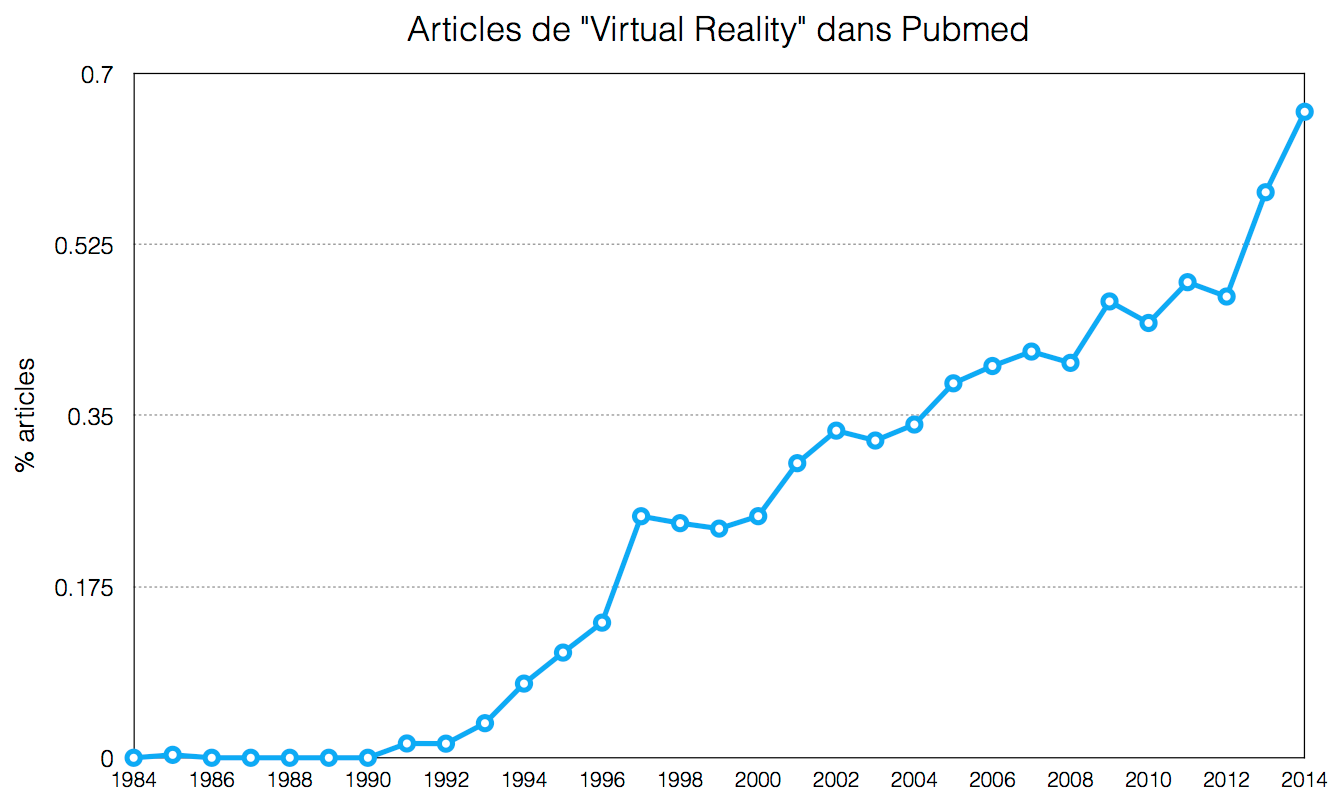
\includegraphics[width=.75\linewidth]{./figures/ch1/VR_pubmed_trend.png}}
    \caption[Évolution des articles traitant de Réalité Virtuelle dans PubMed.]{\it Évolution du pourcentage d'articles de PubMed où le terme <<Virtual Reality>> est retrouvé soit dans le titre soit dans le résumé au cours des 20 dernières années.}
  \label{Fig:VR_pubmed_trend}
  \hspace{0.2cm}
\end{figure}

\section{Perspectives et nouveaux usages de la biologie structurale} \label{limits_persp_bio_struct}

Par rapport au séquençage permettant d'obtenir la séquence de l'ADN d'un organisme de ses gènes et donc de ses séquences protéiques, la biologie structurale a pris du retard pour caractériser la structure tridimensionnelle des protéines dont la séquence a déjà pu être identifiée de façon systématique et fiable. Pour preuve l'écart entre le nombre de protéines dont la séquence est déposée dans UniProtKB\footnote{\url{http://www.uniprot.org/uniprot/}} et le nombre de protéines possédant effectivement une structure déposée dans PDB\footnote{\url{http://www.rcsb.org/}}: Aujourd'hui, seul 1\% des protéines séquencées possèdent une structure répertoriée dans la PDB. 

Pour combler ce retard, les techniques expérimentales et computationnelles ont franchi des paliers, générant de grandes quantités de modèles d'une complexité en constante progression. En effet, la taille des structures moléculaires observées et étudiées augmente régulièrement et il est maintenant possible de simuler des systèmes de plusieurs millions d'atomes pendant des durées biologiques suffisamment longue permettant d'observer des phénomènes biologiques auparavant inaccessibles. La taille et la vitesse du flux de données généré par les outils de modélisation moléculaire dépassent désormais les capacités d'analyses des experts et des outils qu'ils utilisent. Même si les progrès portés sur la précision des techniques de résolution de structures de protéines ne cessent d'augmenter, une attention toute particulière est maintenant portée sur les étapes d'analyse et de visualisation de structures.

La visualisation de capsides virales, de ribosomes ou de complexes membranaires entiers demande des performances importantes de la part des logiciels de visualisation. Ces derniers ont donc dû s'adapter et évoluer pour répondre à ces nouveaux défis en terme de rendu visuel. Le calcul sur processeur graphique a permis de franchir une grande étape en terme de performance et plusieurs algorithmes de rendus graphiques largement utilisés au sein des logiciels de visualisation en ont profité \cite{chavent_gpu-powered_2011}. En parallèle, de nouvelles techniques de rendus graphiques, inspirées pour certaines du monde du jeu vidéo, ont vu le jour afin de rapprocher les représentations de molécules de représentations d'objets réels, facilitant ainsi la perception des objets observés \cite{lv_game_2013}. Les progrès effectués en terme de performance ont également permis de rendre la visualisation moléculaire interactive,  accordant ainsi aux utilisateurs davantage de possibilités quant à leurs options de rendus et dépassant ainsi la simple image statique et précalculée de structure 3d.

Cependant, ces récentes avancées ne sont pas suffisantes pour appréhender la complexité des complexes moléculaires étudiés aujourd'hui. La limitation n'est pas dans l'efficacité du rendu, mais dans la façon d'explorer les structures 3d d'intérêt d'interagir avec elles. Il s'avère que la Réalité Virtuelle dispose d'une large gamme de techniques pour naviguer et interagir dans des scènes 3d complexes, dont certaines sont déjà appliquées pour faciliter notamment l'étape de modélisation et de simulation.

\clearpage

% \begin{eqnarray}
% \left\{ \begin{array}{ll}
% 	F_1(V\!E=0.8)=&F1 \\
% 	F_1(V\!E=0.6)=&0.925F1\\
% 	F_1(V\!E=1.0)=&1.075F1\\
% \end{array} \right.
% \end{eqnarray}

% \begin{eqnarray}
% F_1(V\!E)=
% \left\{
% 	\begin{array}{lll}
% 		&(0.7+0.375 \cdot V\!E) \cdot F1& \mbox{ si $V\!E\geq0.6$}\\
% 		&0.925 \cdot F1& \mbox{ si $V\!E<0.6$}\\
% 	\end{array}
% \right.
% \end{eqnarray}

% \begin{equation} 
% \begin{split}
% b_{TL} & = 1 - \nu + \sqrt{\nu^2-1}\\
% \nu    & = 1-\frac{1}{\eta} \\
% \eta   & = \frac{10^{TL/10}-1}{\cos(2\pi\frac{3000}{F_e})-1}
% \end{split} 
% \end{equation} 

% \begin{eqnarray} 
% \vert H( e^{2i \pi fc /F_e}) \vert = \frac{\vert H(1) \vert}{ \sqrt[]{2}}  \label{Eqa:1}
% \end{eqnarray}


% \noindent En élevant au carré (\ref{Eqa:1}), on obtient :
 
% \begin{eqnarray} 
% 	\frac{b_{TL}^2}{2 \cdot (1-b_{TL})(1-\cos(2i \pi f_c / F_e)) + b_{TL}^2} &=& \frac{1}{2}
% \end{eqnarray}



% \begin{figure}
%   \centering
%   \subfloat
%   [{\it Sans dépendance}]
%   {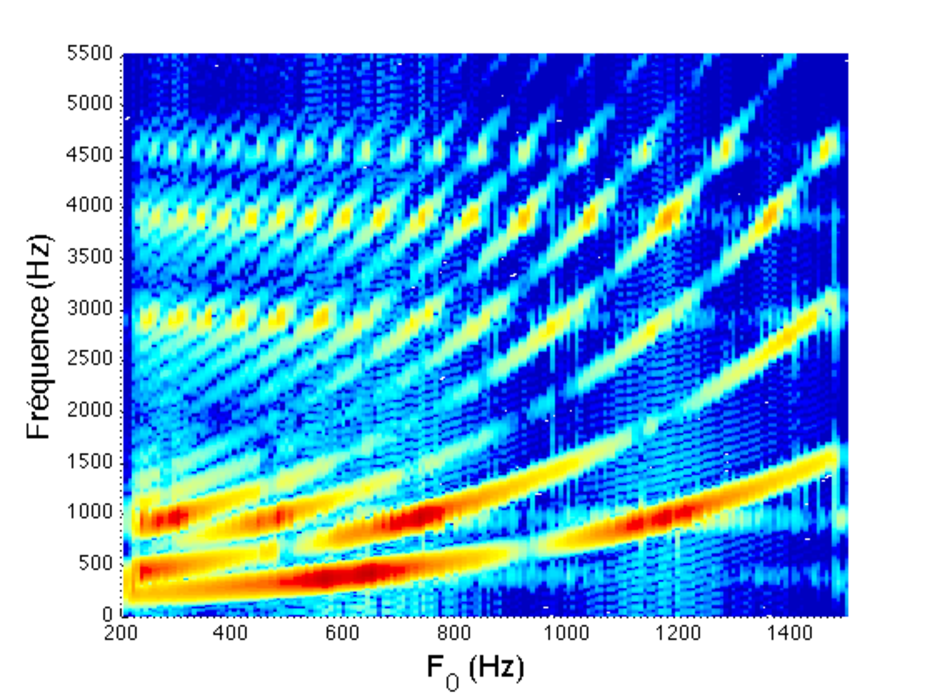
\includegraphics[width=.45\linewidth]{ch2/fig/Fi-F0-dpdce-sans_soprano_u_200-1500Hz_dig13b3.pdf}}
%   \label{Fig:Fi-F0-dpdce_sans}
%   \hspace{0.2cm}
%   \subfloat
% 	[{\it Avec dépendances}]  
%   {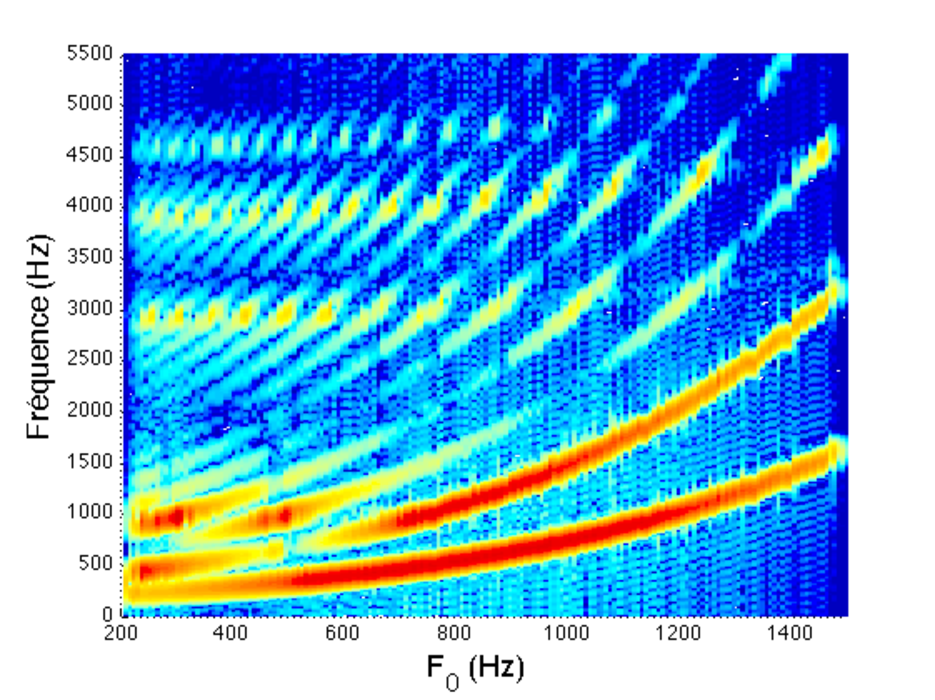
\includegraphics[width=.45\linewidth]{ch2/fig/Fi-F0-dpdce-avec_soprano_u_200-1500Hz_dig13b3.pdf}}
%   \label{Fig:Fi-F0-dpdce_avec}
%     \caption{{\it Spectrogrammes de la voyelle /a/ de synthèse, où $F_0$ augmente avec le temps, (a) sans ou (b) avec les dépendances entre les fréquences centrales des formants et de $F_0$. \textit{Voir fichiers audios~/ vidéos~\ref{fav:fi-f0-dependance}}\\
% }}
%   \label{Fig:Fi-F0-dpdce}
% \end{figure}

% \subsubsection{a) La soufflerie}

% \begin{table}[!h]
% 	\centering
% 	\begin{tabular}{|c|c|c|} 
% 		\hline
% 		& \centering \textbf{Tessiture naturelle moyenne} & \centering \textbf{Tessiture
% dans le synthétiseur} \tabularnewline
% 		\hline
% 		\bf Basse & Mi2-Mi4 & Sol$\sharp$1-Sol4\\
% 		\hline
% 		\bf Ténor & Do3-Si4 & Sol$\sharp$1-Sol4\\
% 		\hline
% 		\bf Alto & Fa3-Mi5 & Sol$\sharp$2-Sol5\\
% 		\hline
% 		\bf Soprano & Si3-Do6 & Sol$\sharp$3-Sol6\\
% 		\hline
% 	\end{tabular}
% 	\caption{\textit{Tessiture des chanteurs naturels et synthétiques (La3=440 Hz). Voir fichiers audios~/ vidéos~\ref{fav:types-voix-1}}}
% 	\label{Tab:tessChant}
% \end{table}

